\cleardoublepage
%%%%%%%%%%%%%%%%%%%%%%%%%%%%%%%%%%%%%%%%%%%%%%%%%%%%%%%%%%%%%%%%
\chapter{Coverage of the uncertainty with the sFit}
\label{app:Bootstrapping}
%%%%%%%%%%%%%%%%%%%%%%%%%%%%%%%%%%%%%%%%%%%%%%%%%%%%%%%%%%%%%%%%

Figures below show the distributions of the parameters from the fit. together with their corresponding pull distributions, obtained when performing the bootstrapping test, for both simulation (\figref{fig:Pulls_MC} and \figref{fig:Vars_MC}), data (\figref{fig:Pulls_Data} and \figref{fig:Vars_Data}), and simulation of signal and background (\figref{fig:Pulls_MCwBkg} and \figref{fig:Vars_MCwBkg}).

\begin{figure}[tb]
   \begin{center}
	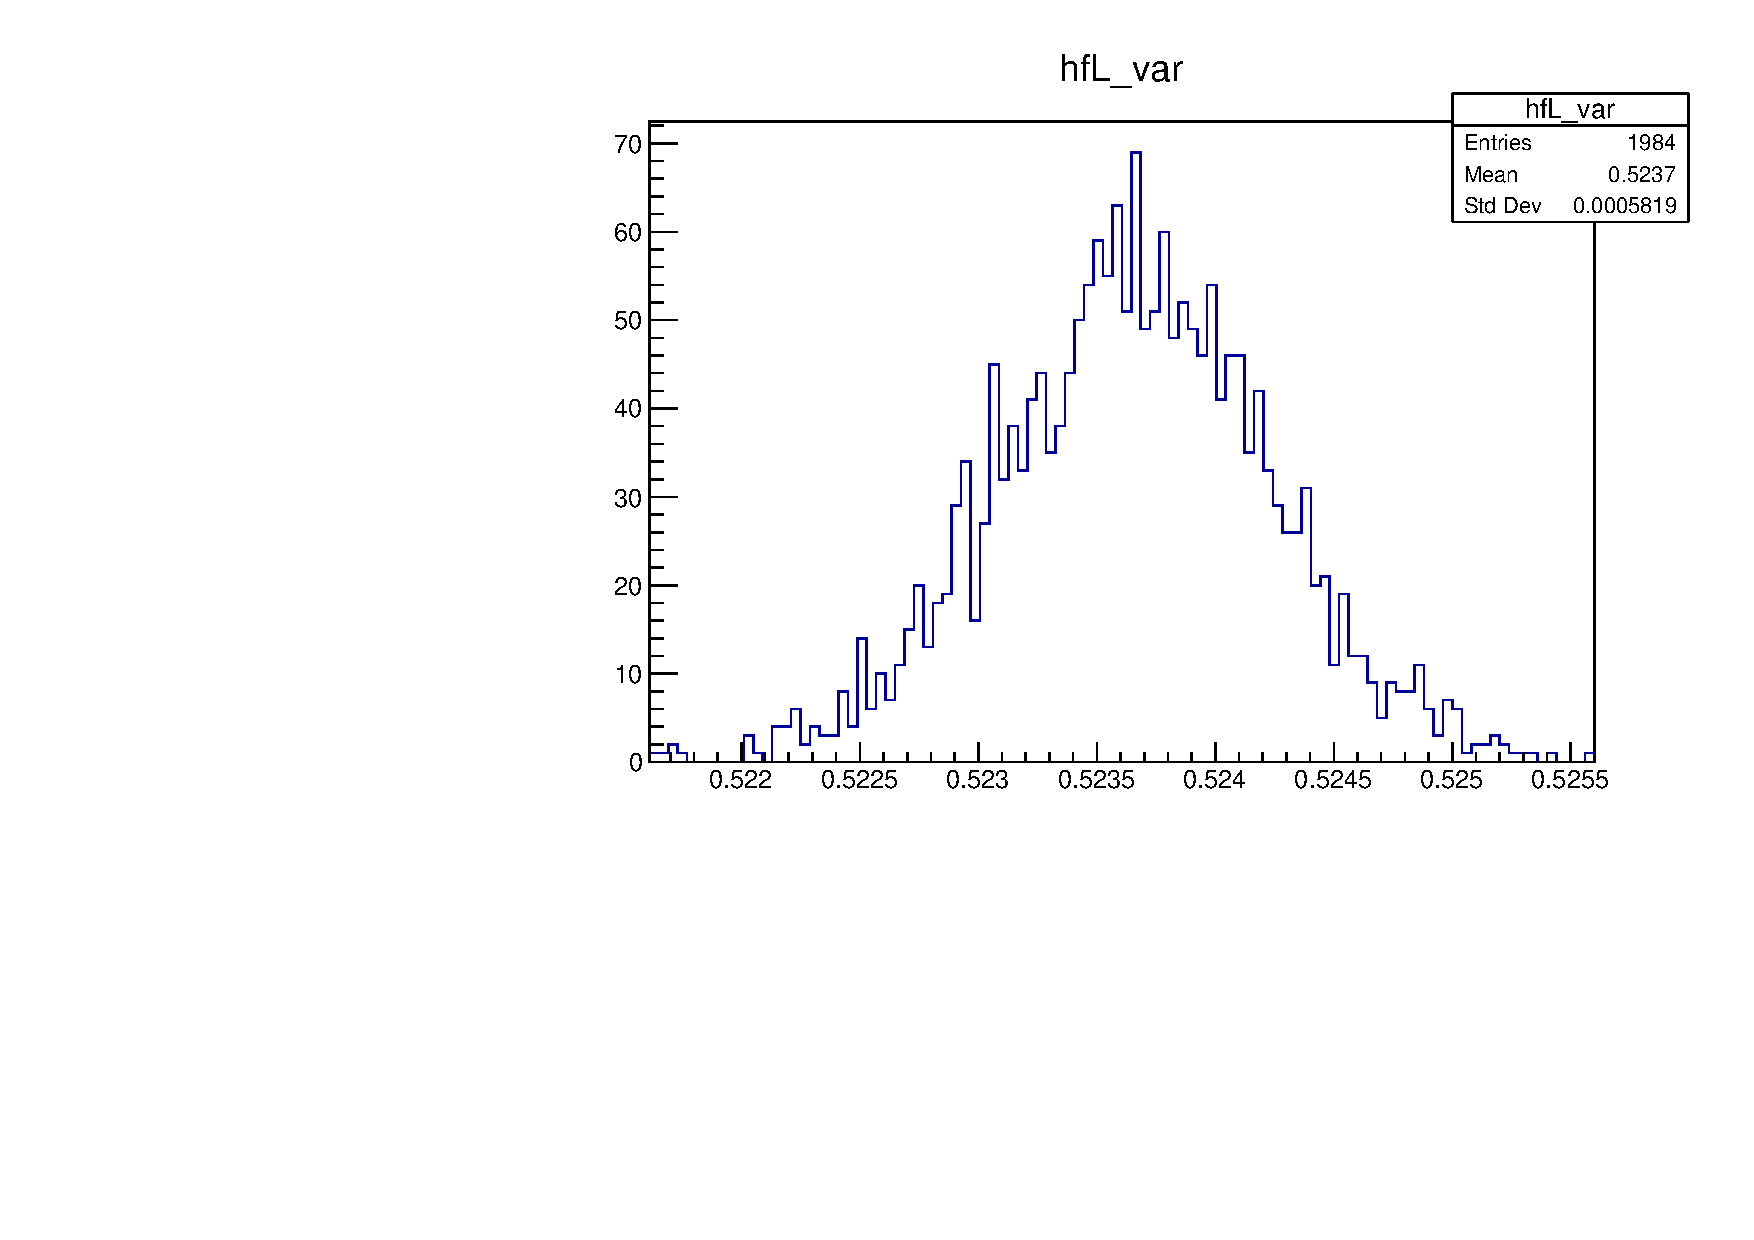
\includegraphics[width=0.3\textwidth]{figs/MCVars/fL_var.pdf}
	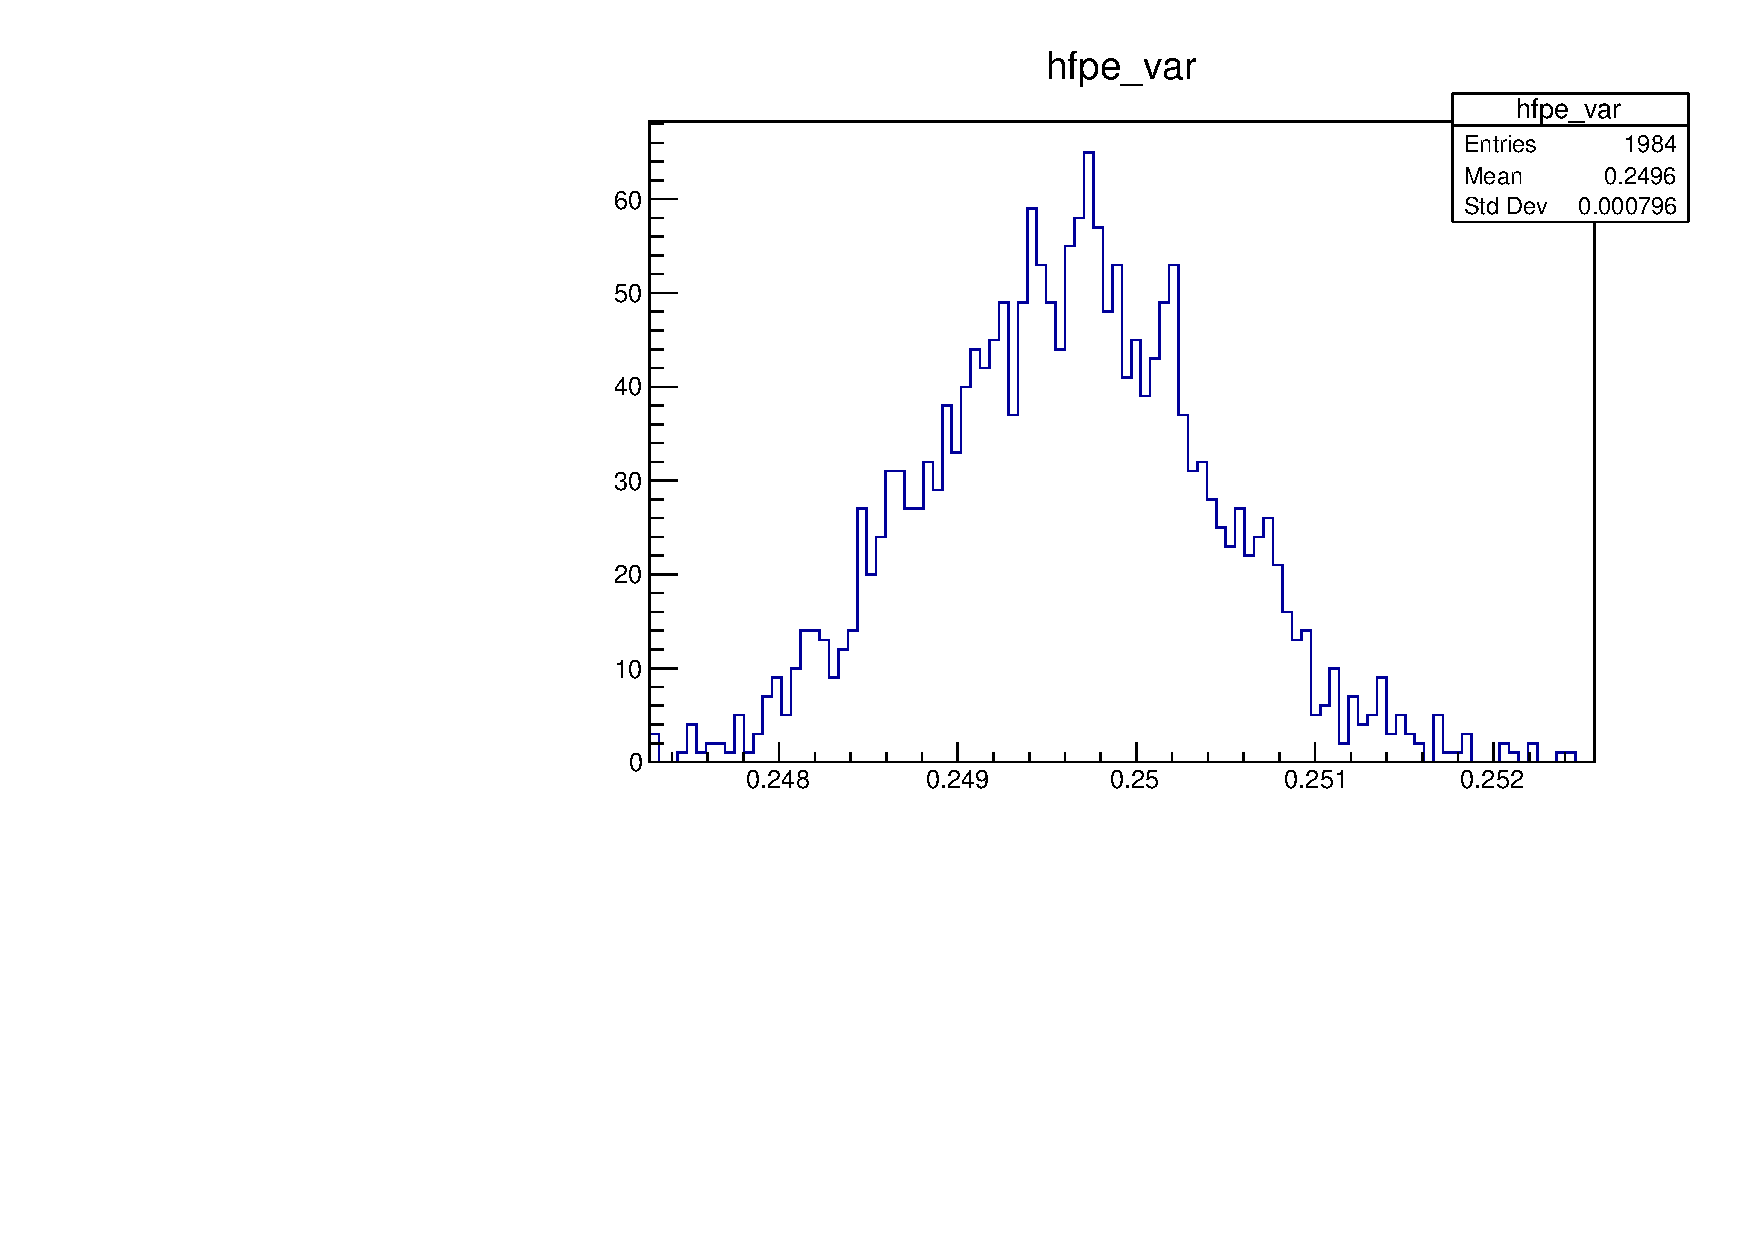
\includegraphics[width=0.3\textwidth]{figs/MCVars/fpe_var.pdf}
	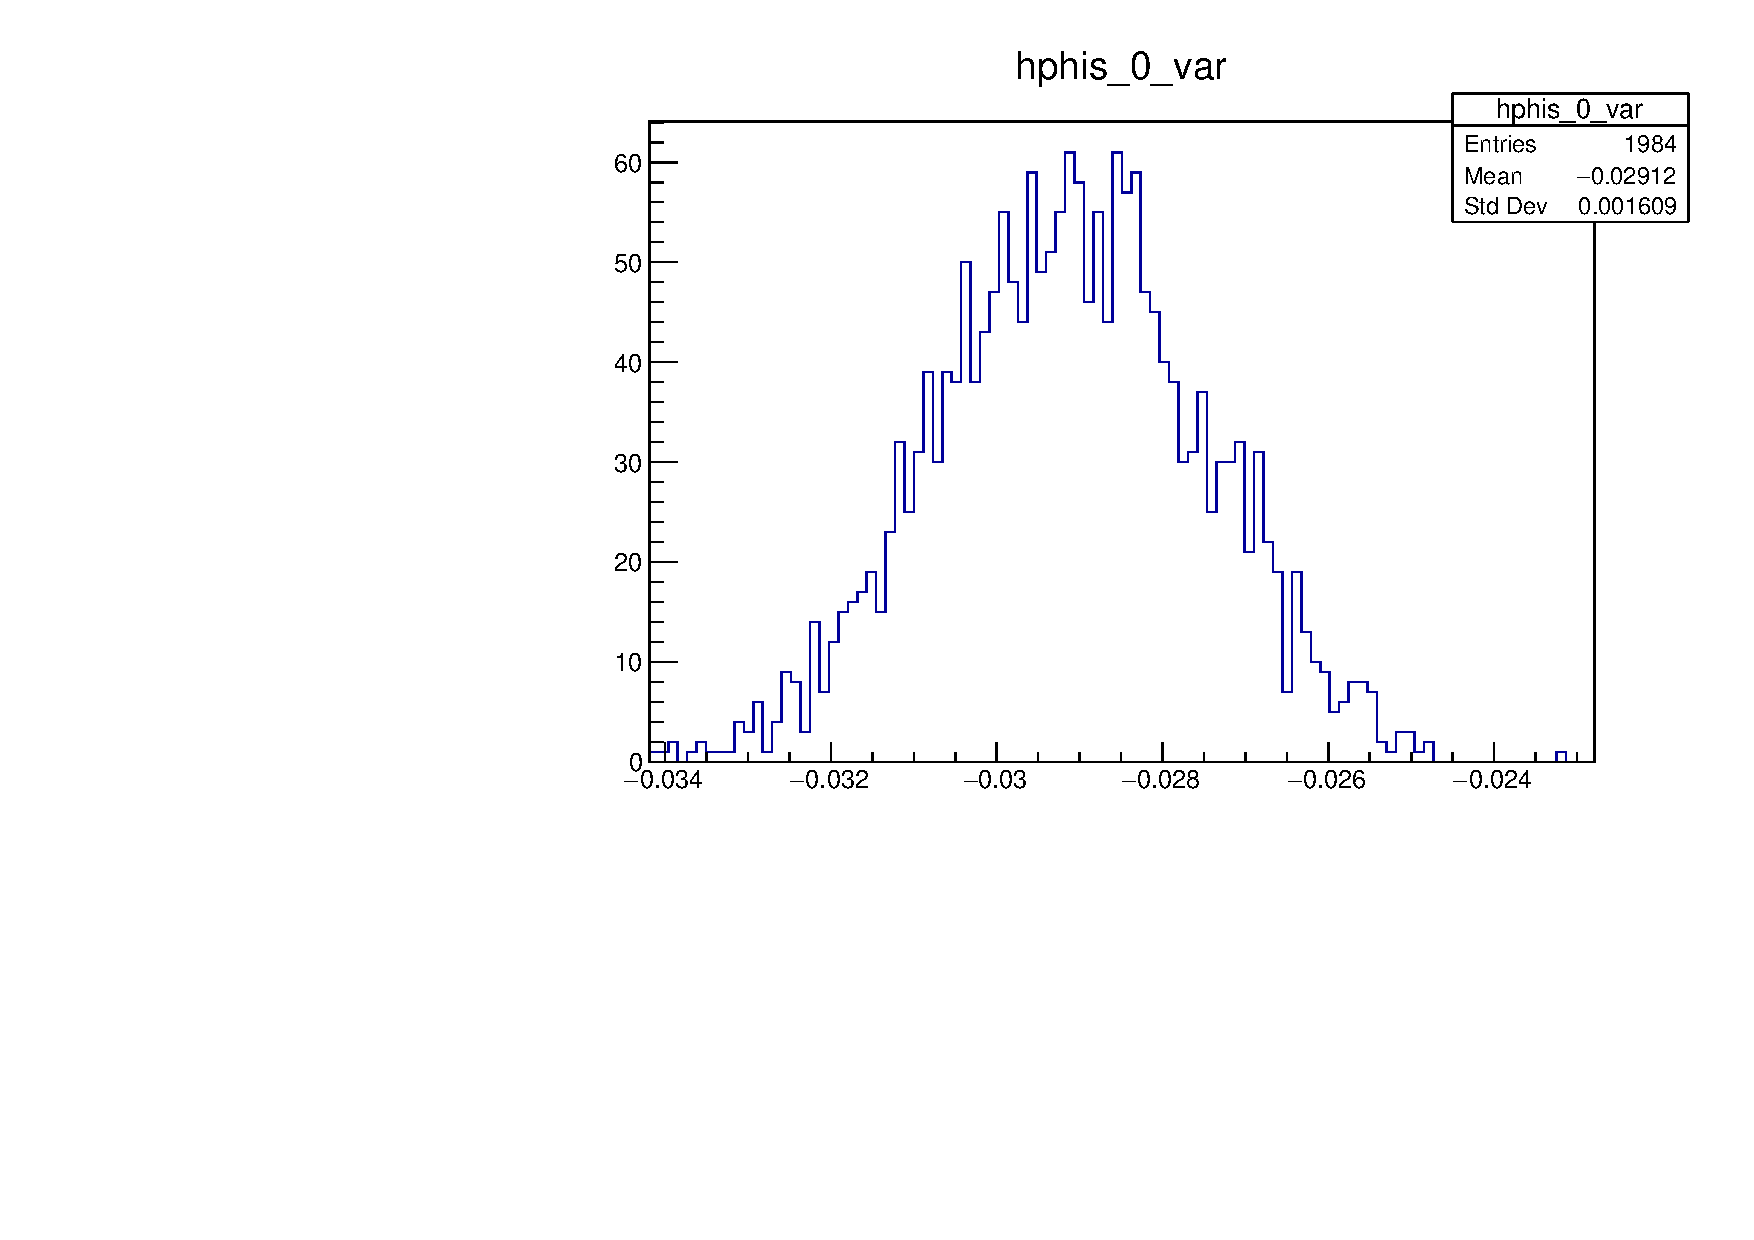
\includegraphics[width=0.3\textwidth]{figs/MCVars/phis_0_var.pdf}
	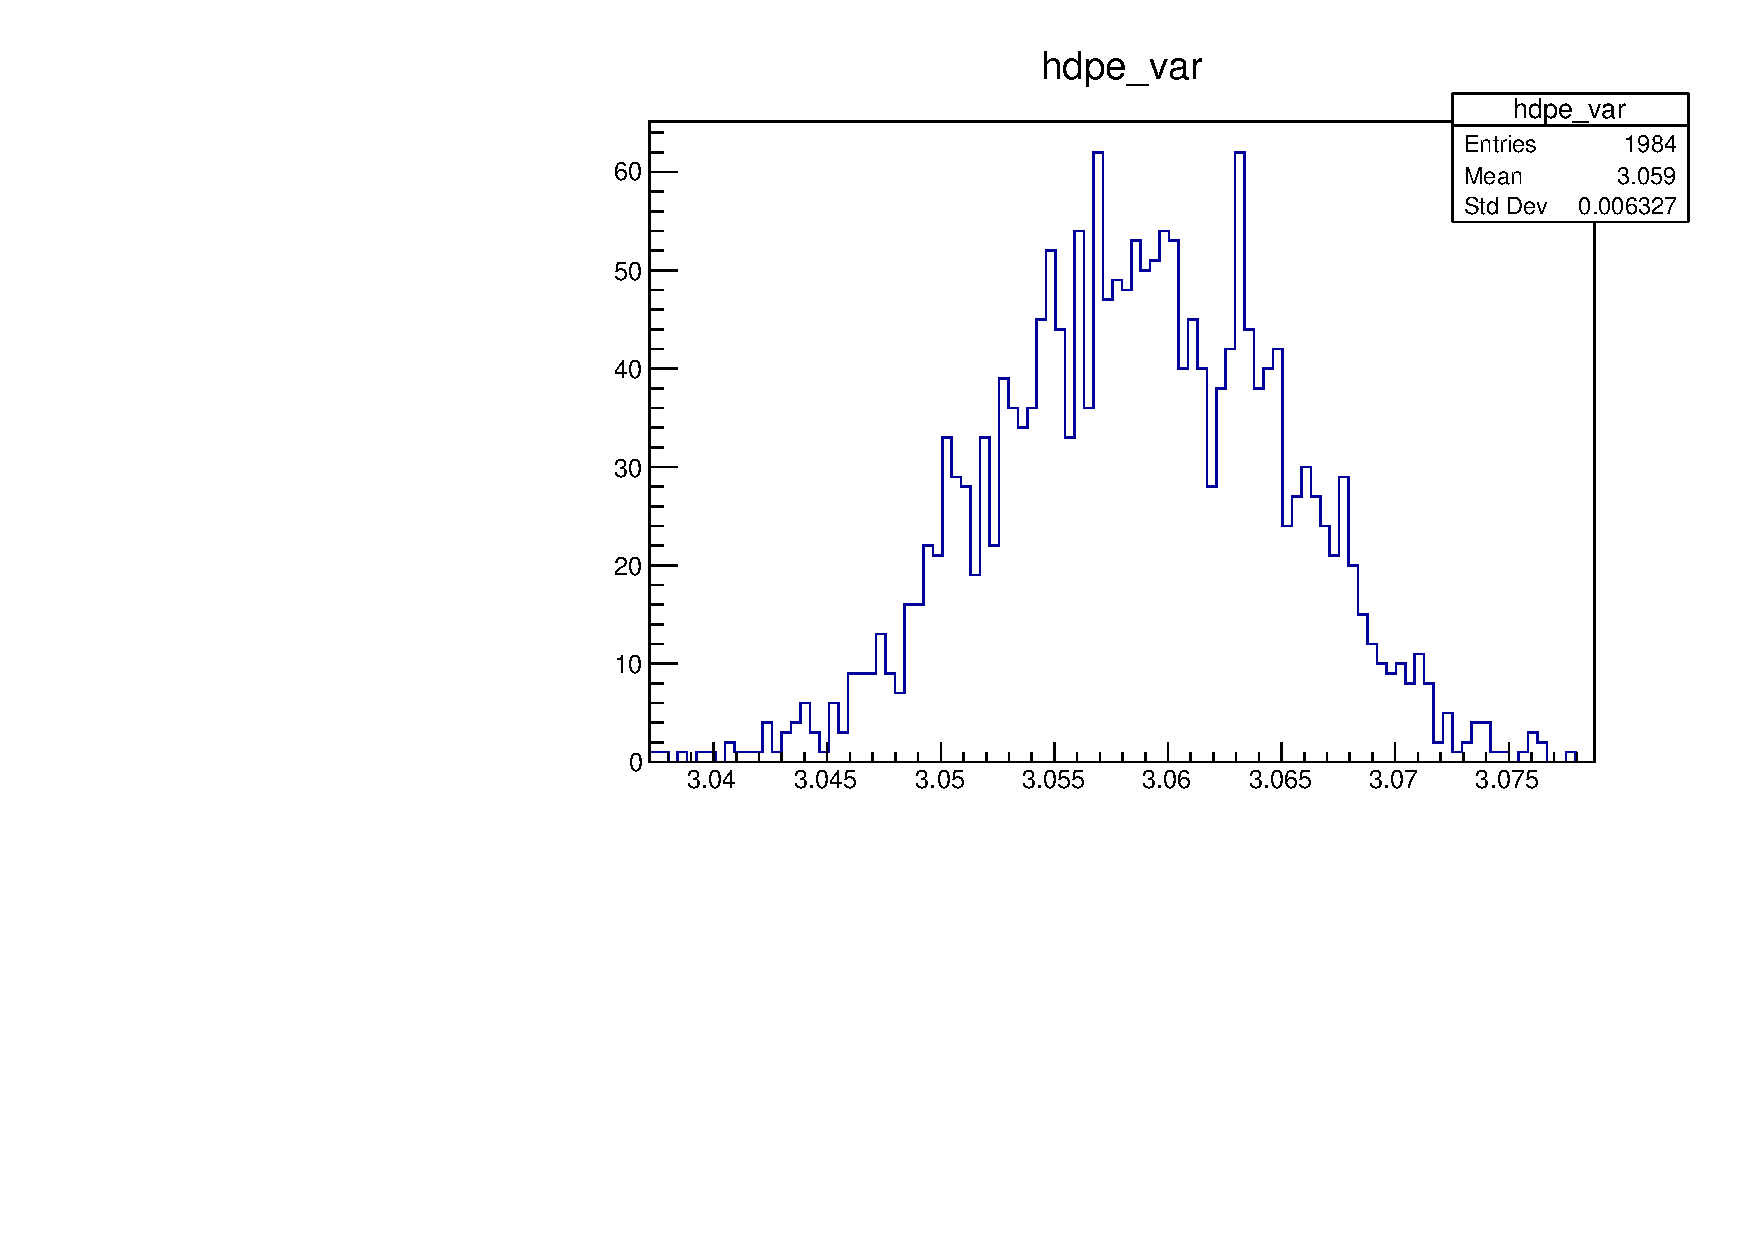
\includegraphics[width=0.3\textwidth]{figs/MCVars/dpe_var.pdf}
	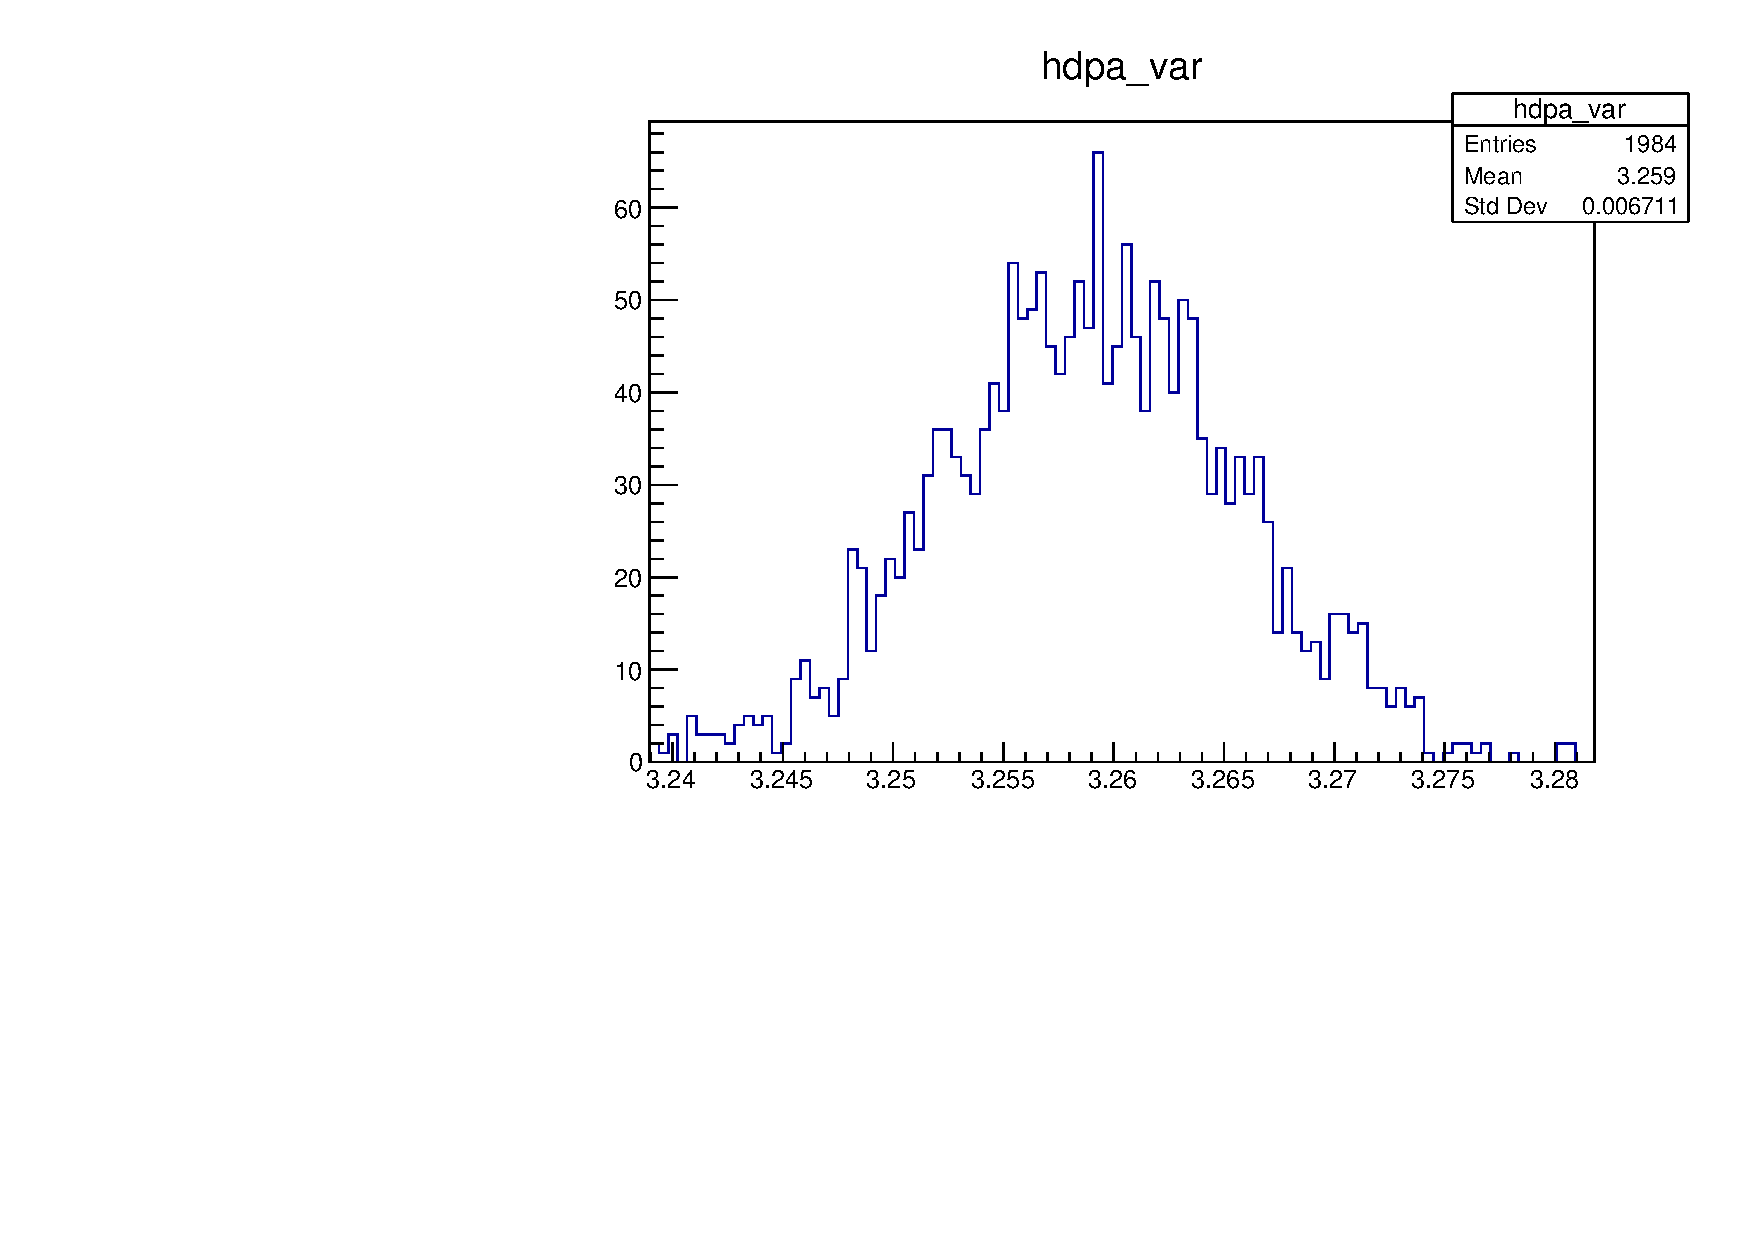
\includegraphics[width=0.3\textwidth]{figs/MCVars/dpa_var.pdf}
	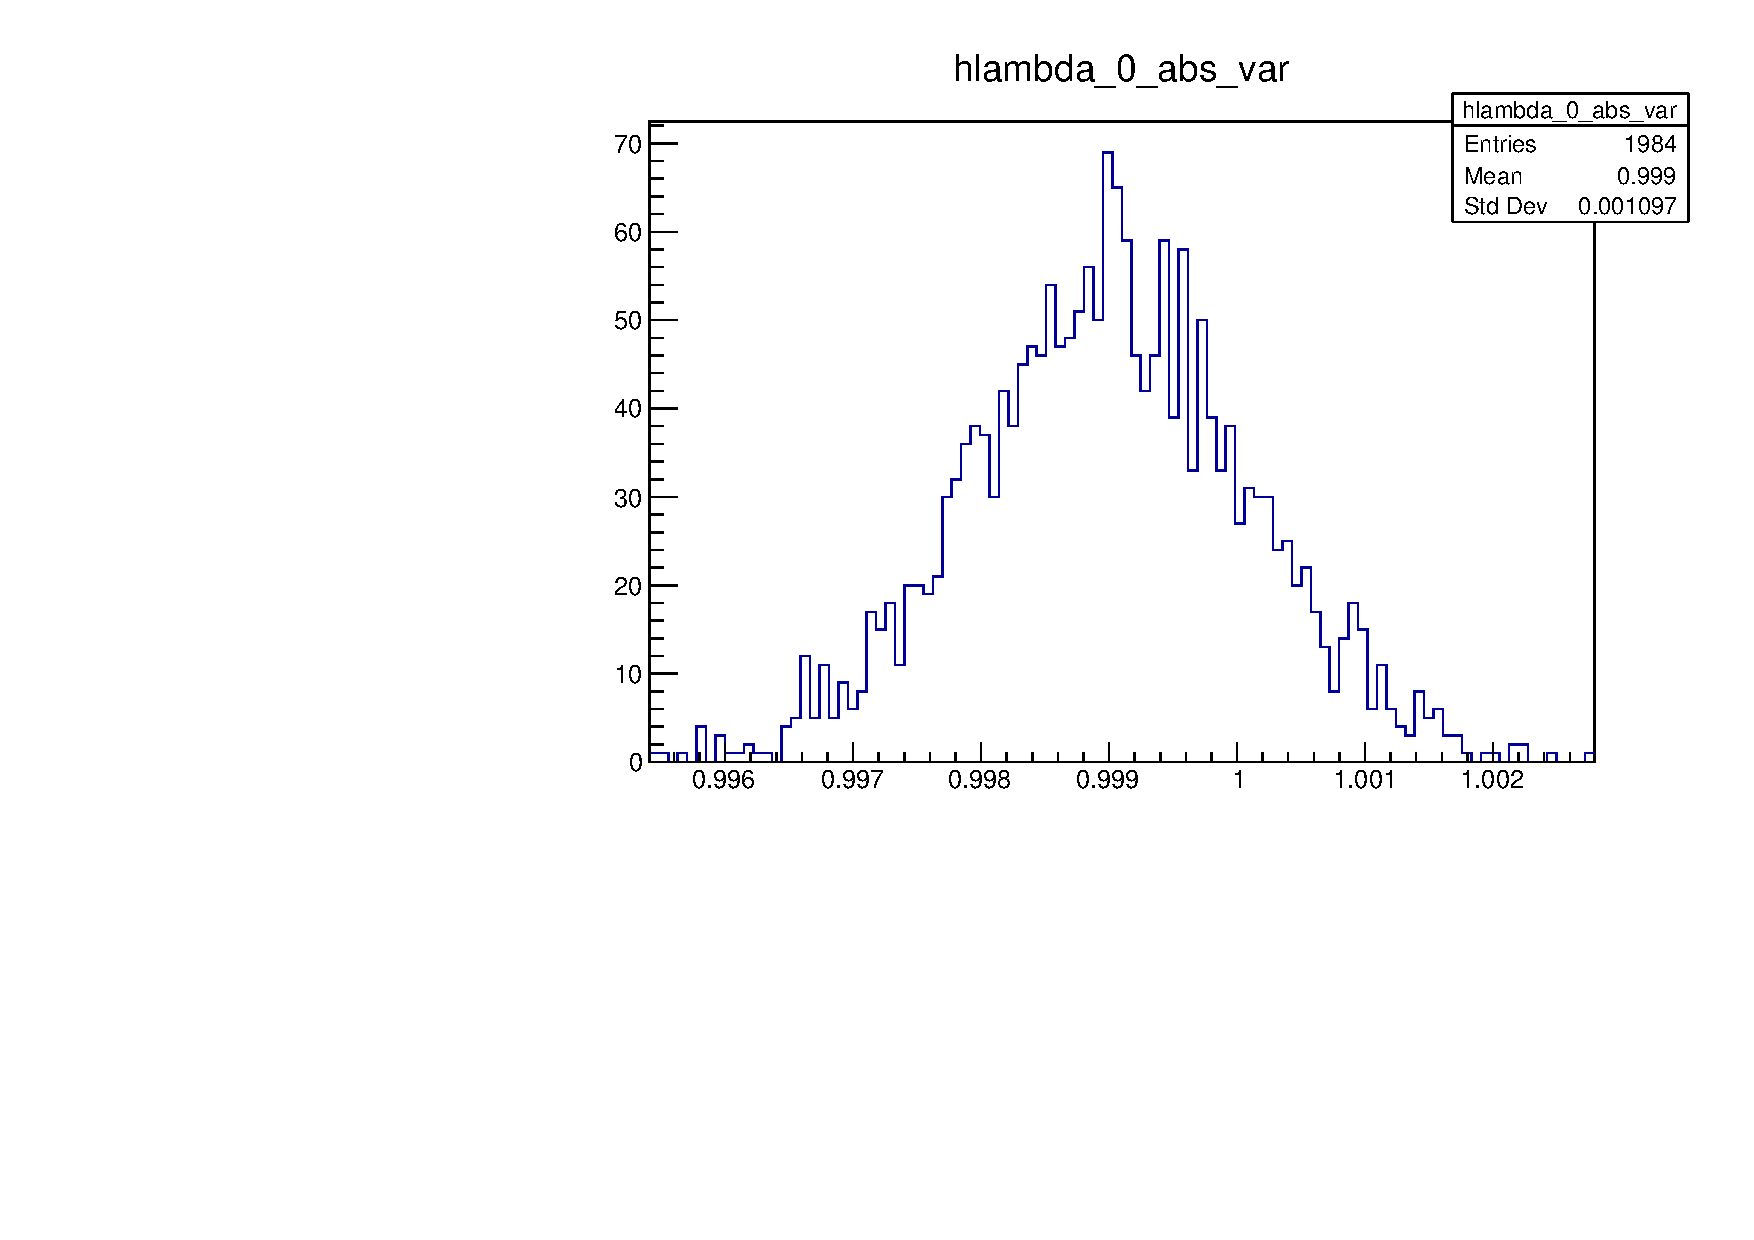
\includegraphics[width=0.3\textwidth]{figs/MCVars/lambda_0_abs_var.pdf}
	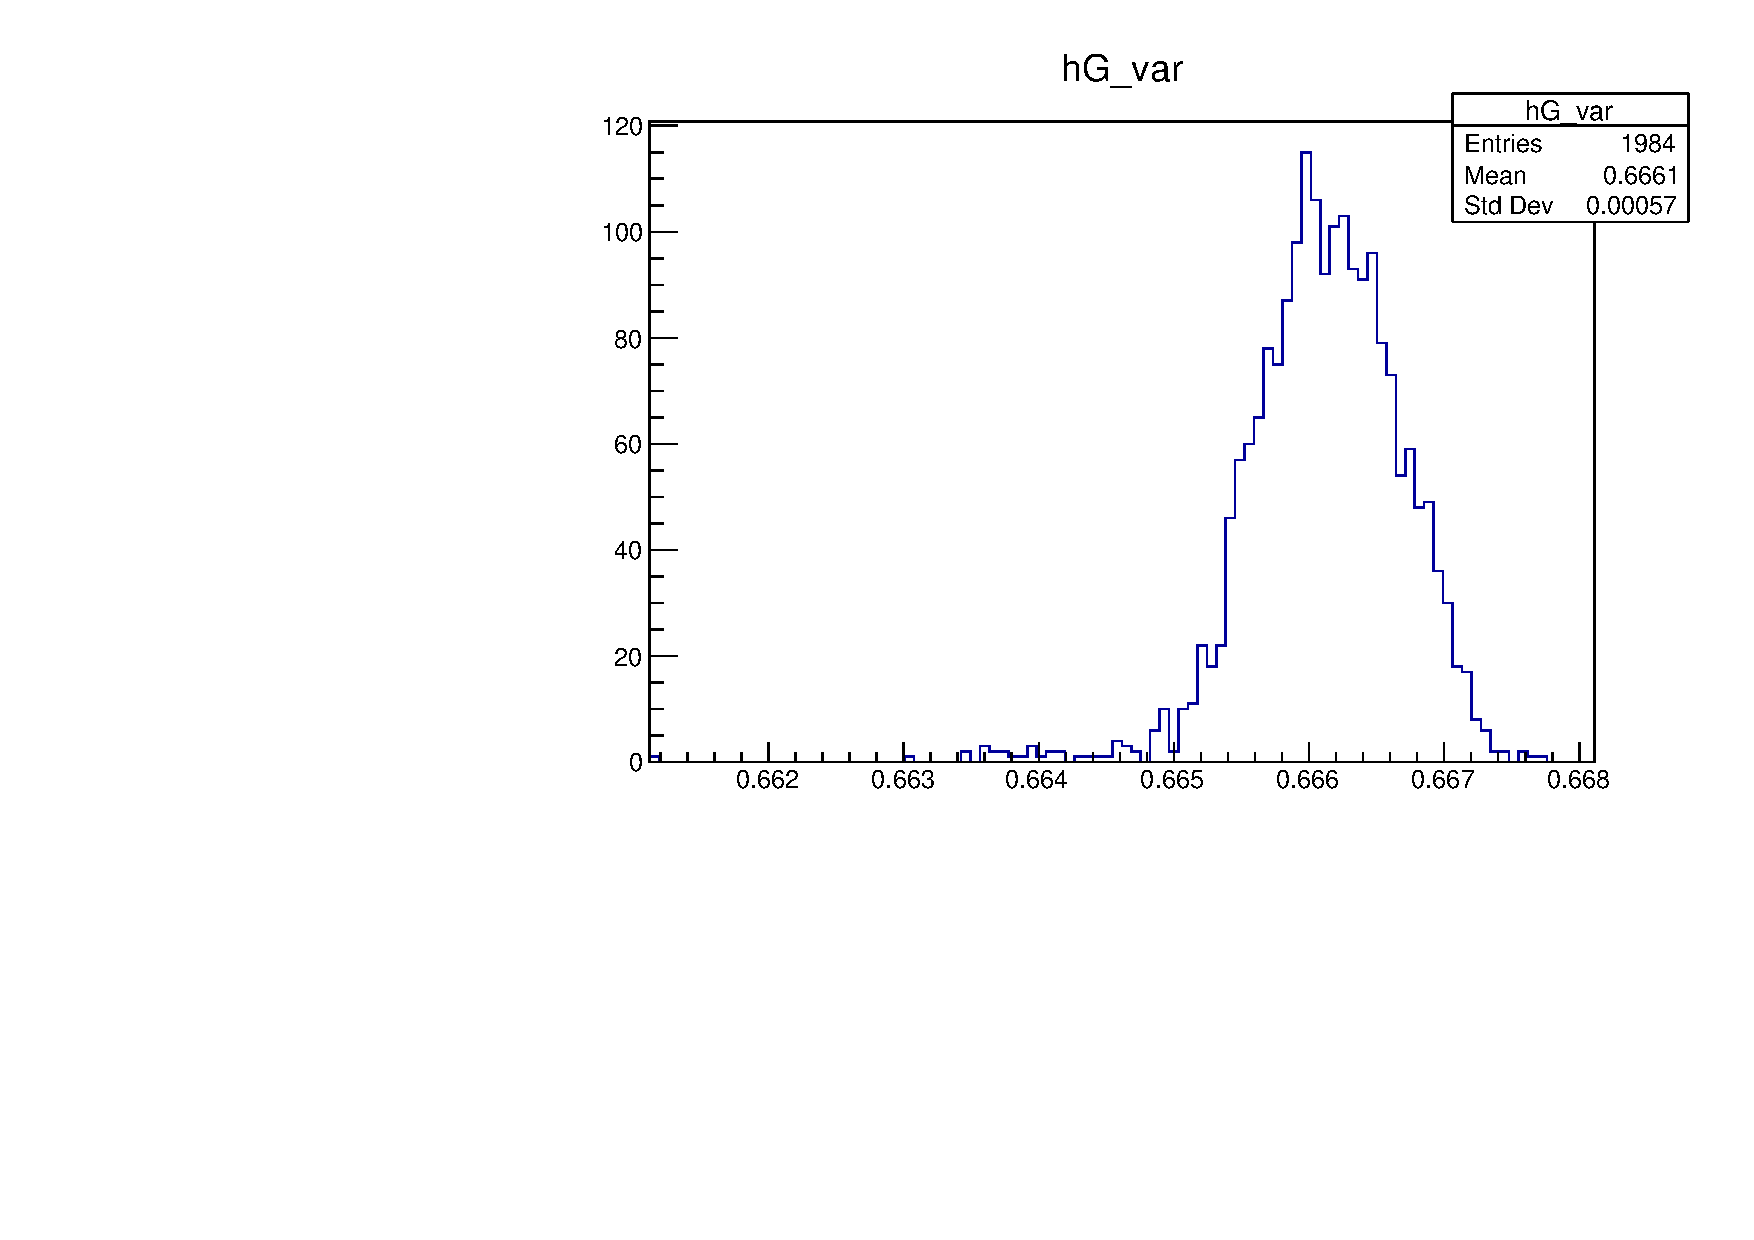
\includegraphics[width=0.3\textwidth]{figs/MCVars/G_var.pdf}
	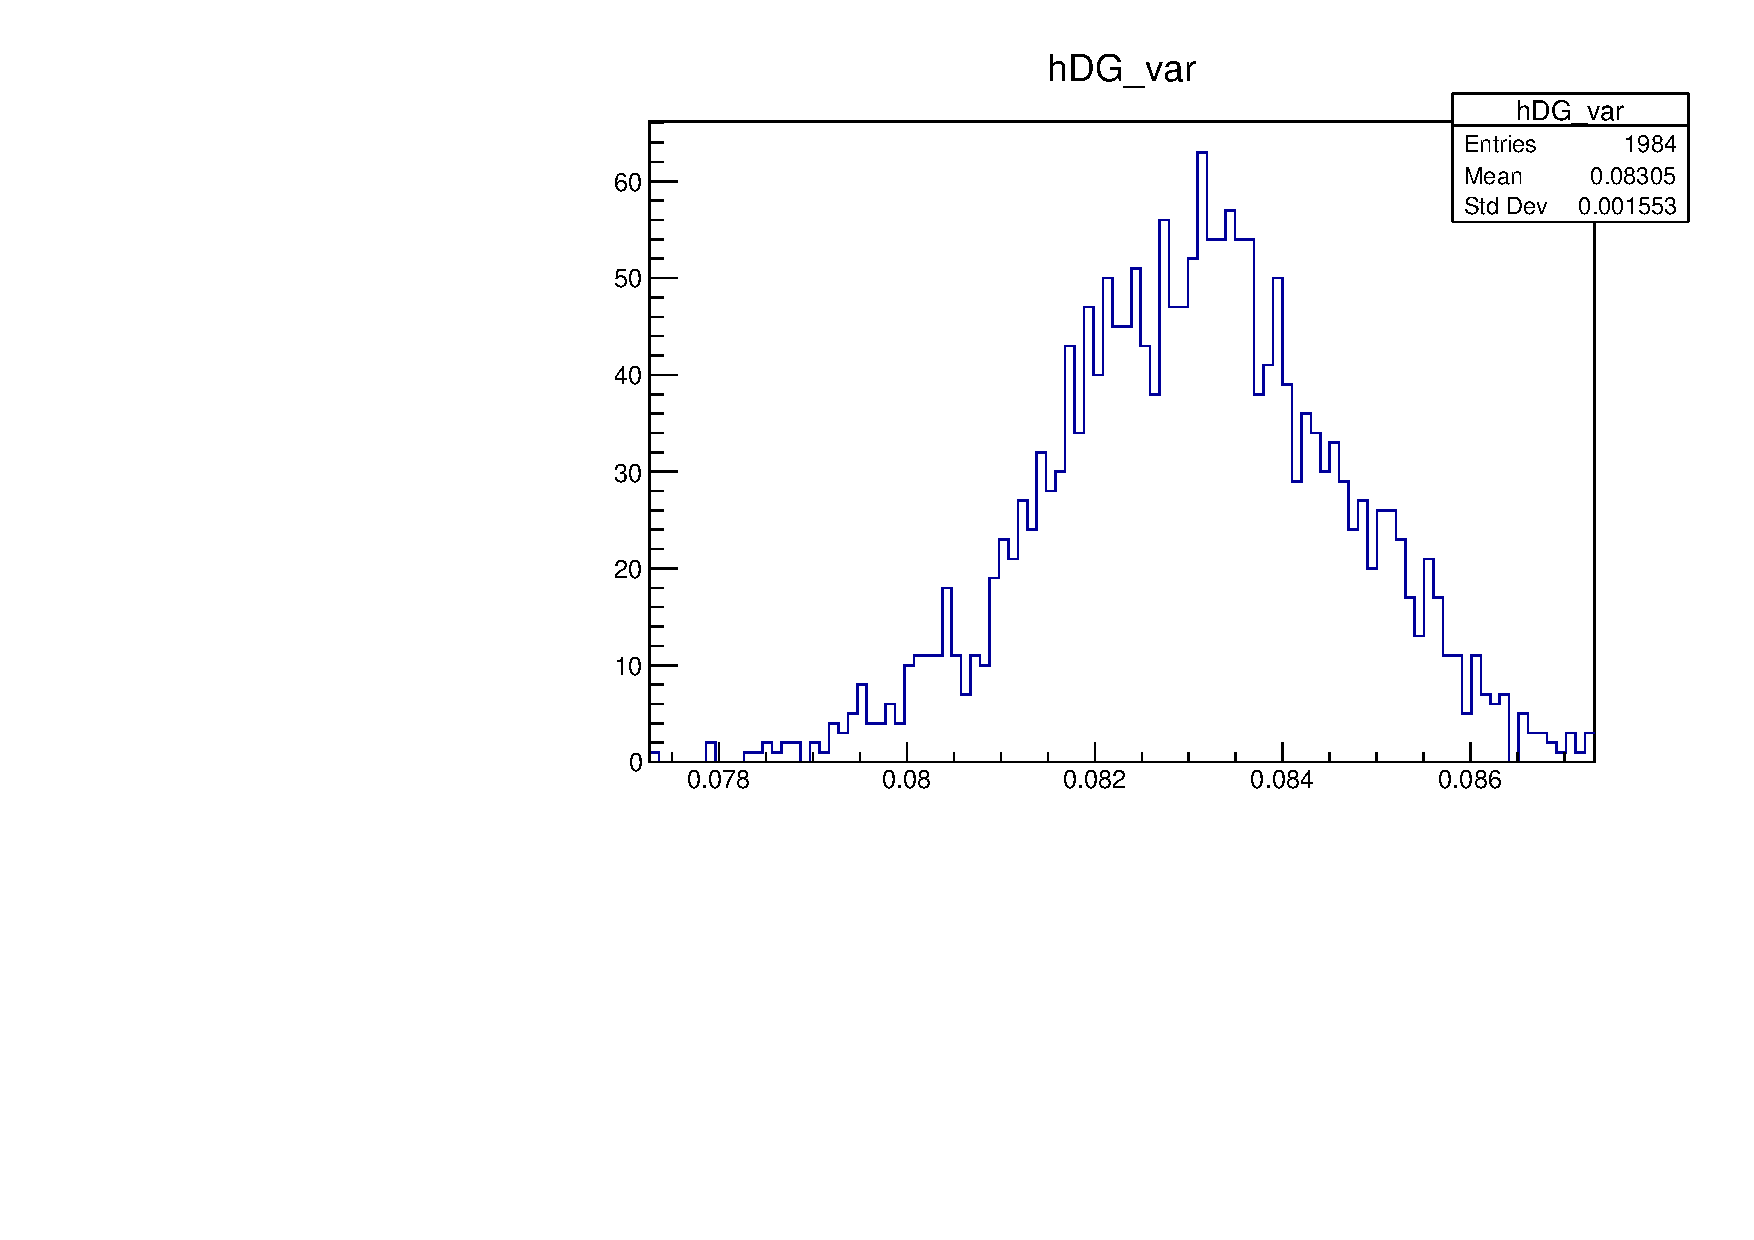
\includegraphics[width=0.3\textwidth]{figs/MCVars/DG_var.pdf}
	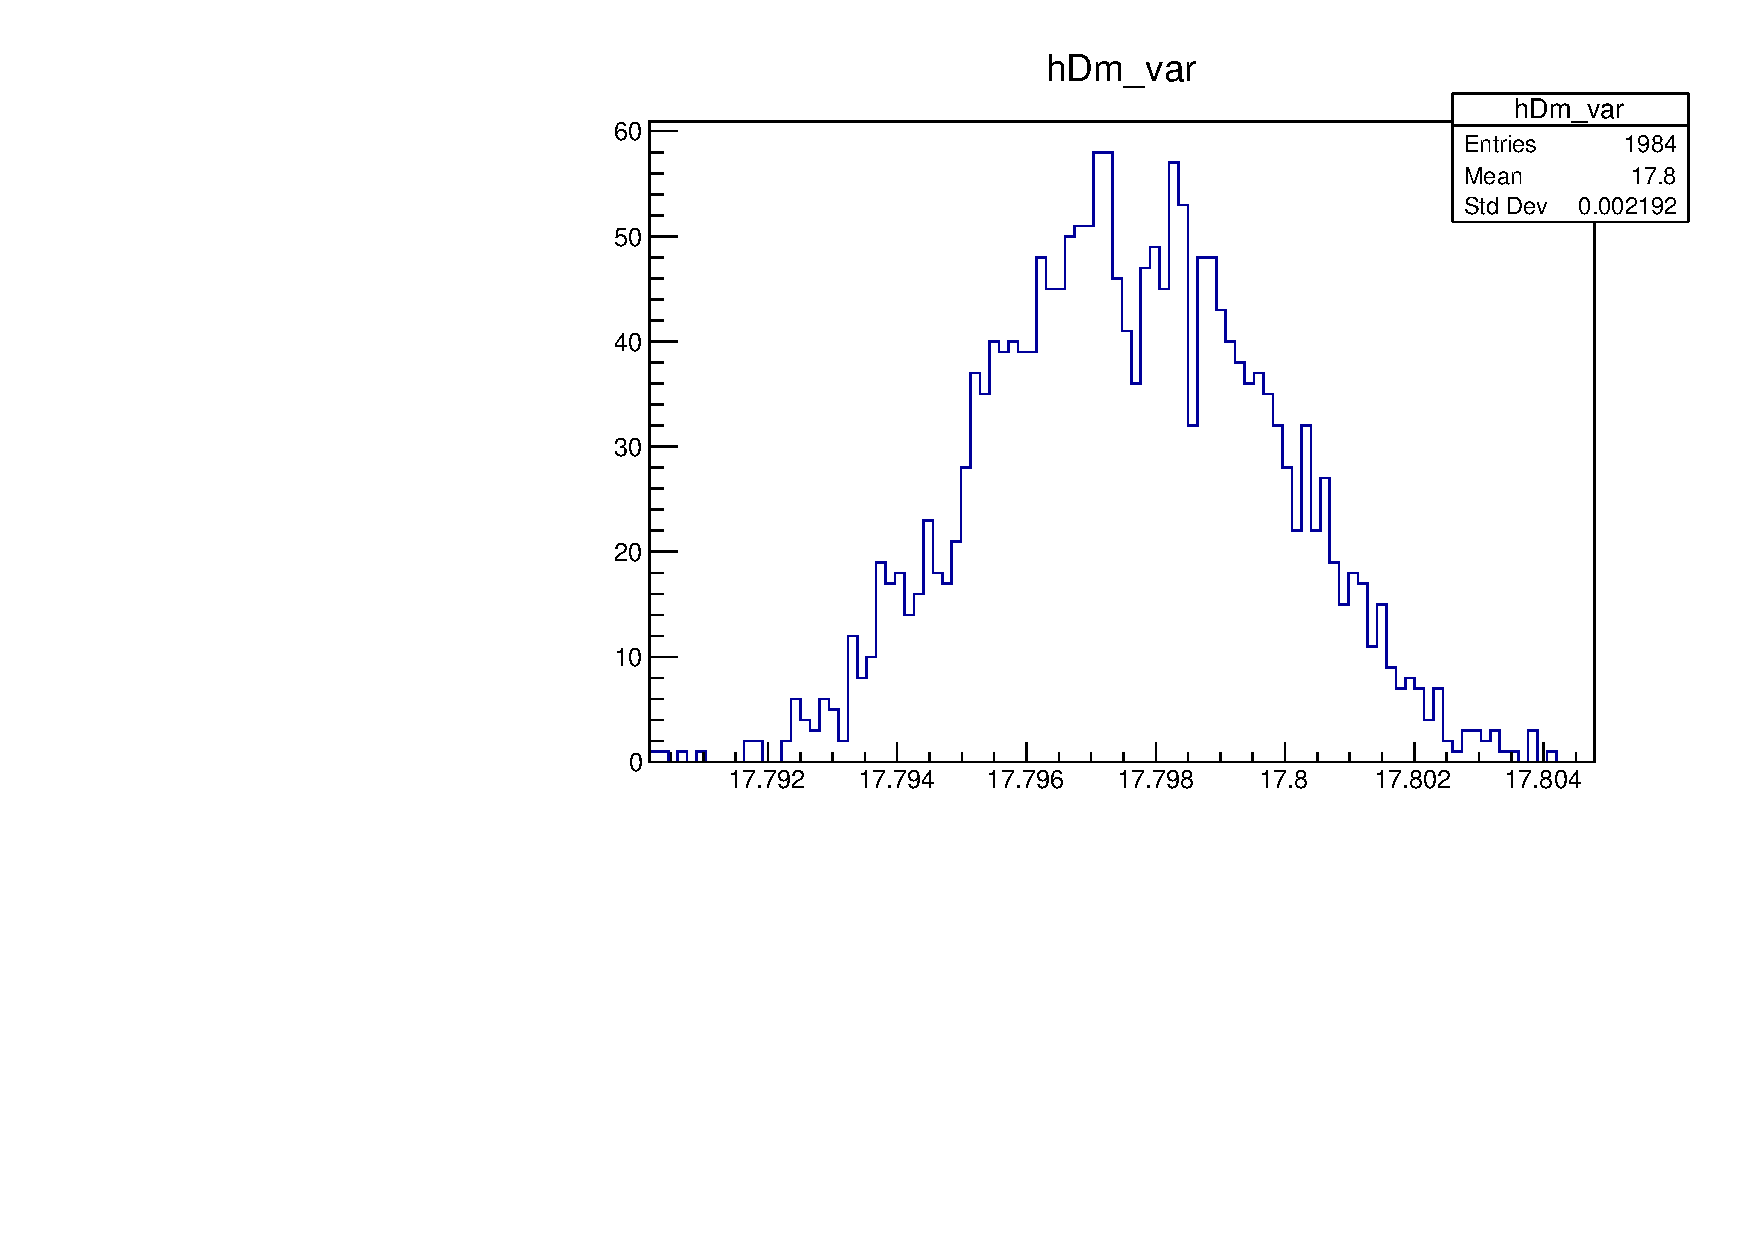
\includegraphics[width=0.3\textwidth]{figs/MCVars/Dm_var.pdf}
   \end{center}
   \caption{
	Distributions of the fit parameters using bootstrapping (MC).
   }
   \label{fig:Vars_MC}
\end{figure}

\begin{figure}[tb]
   \begin{center}
	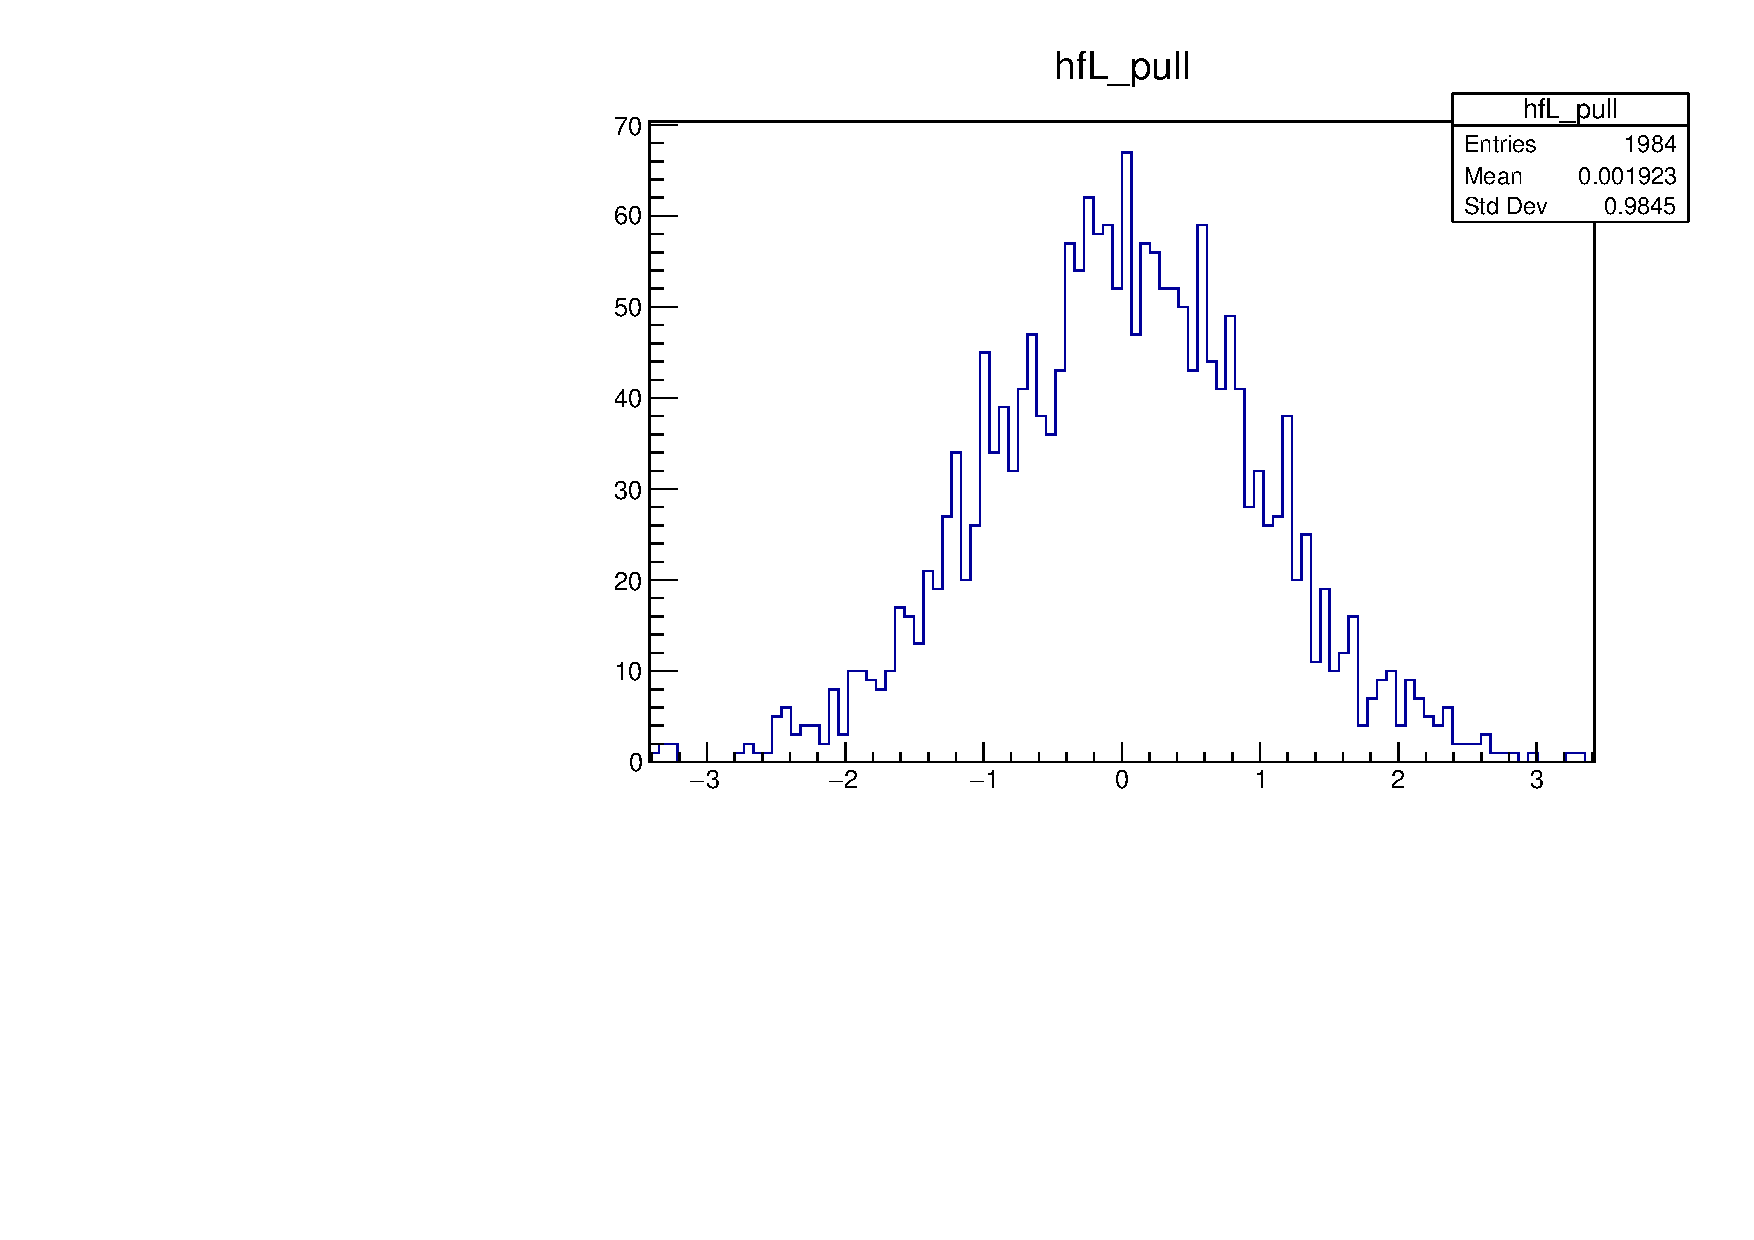
\includegraphics[width=0.3\textwidth]{figs/MCPulls/fL_pull.pdf}
	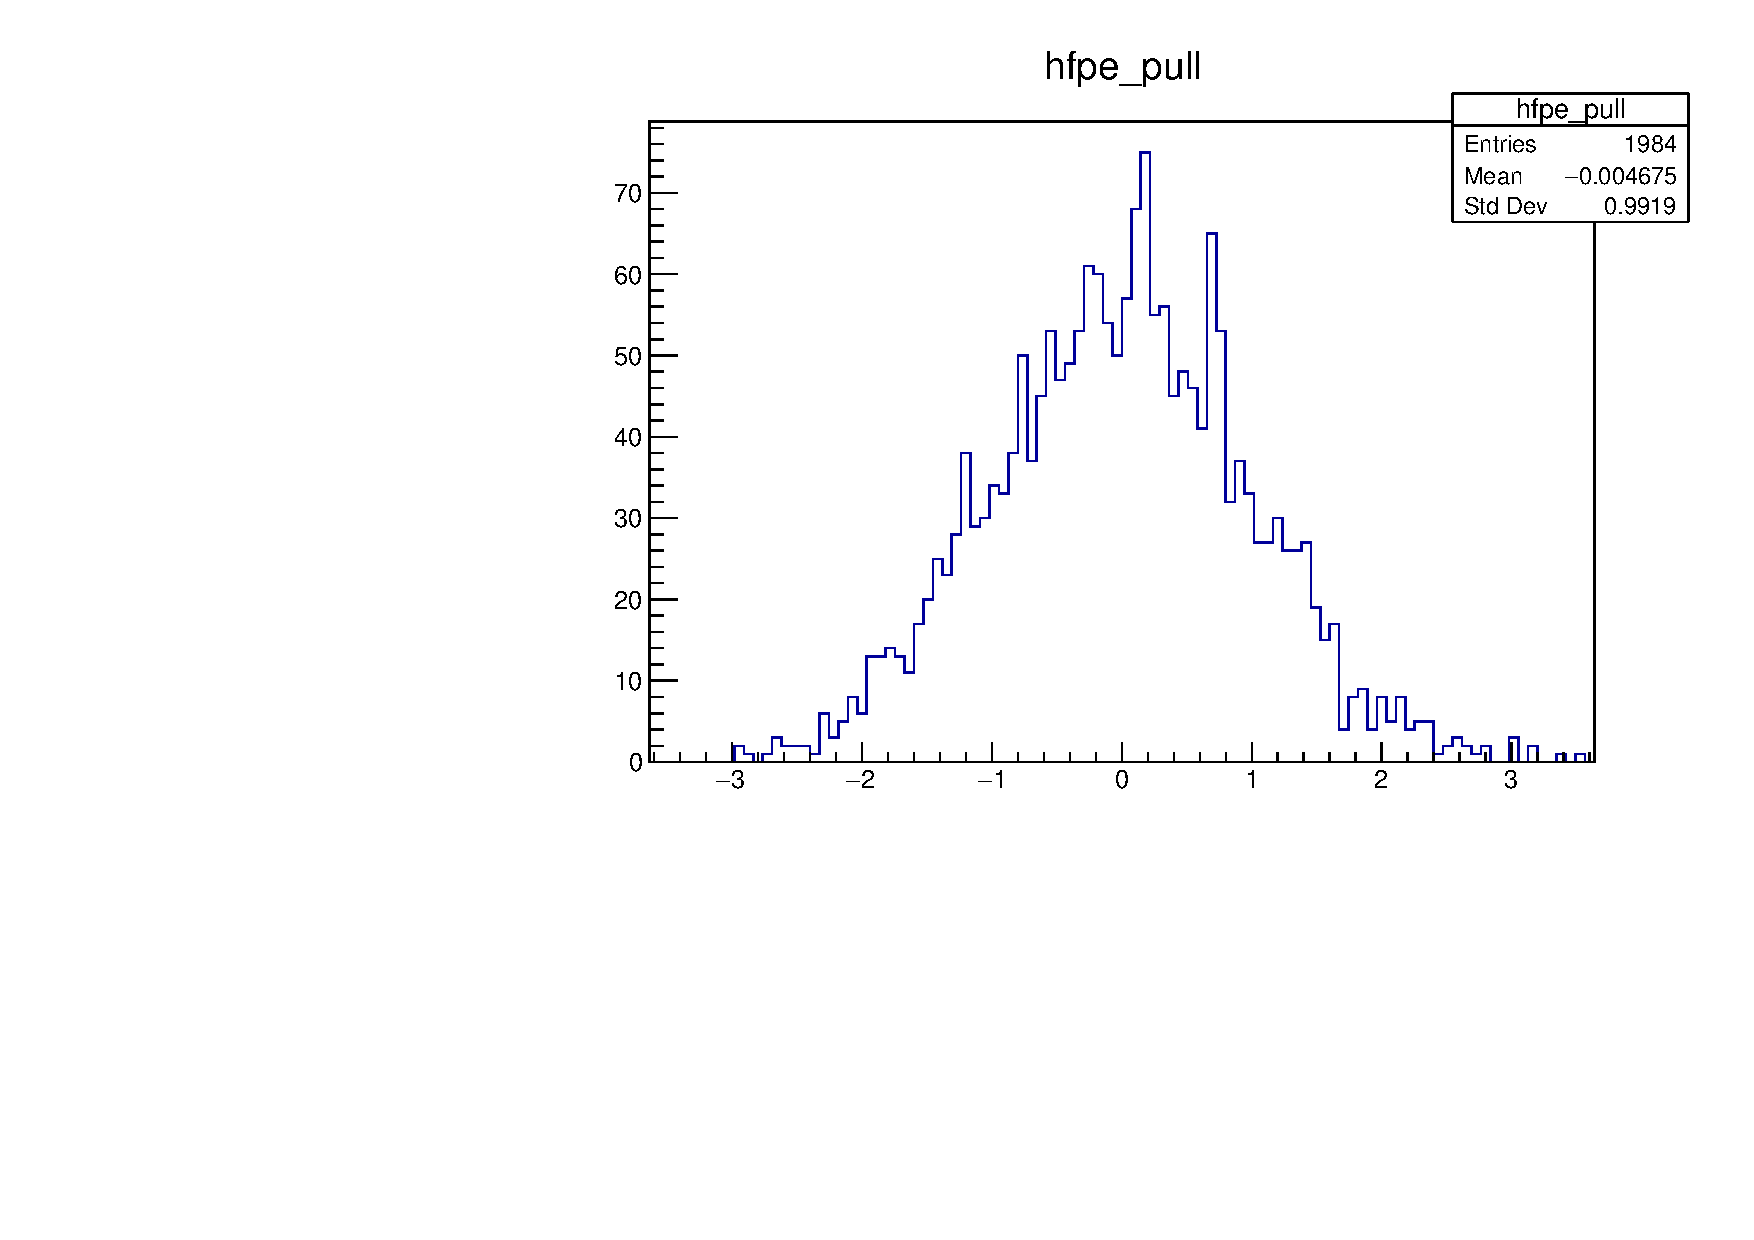
\includegraphics[width=0.3\textwidth]{figs/MCPulls/fpe_pull.pdf}
	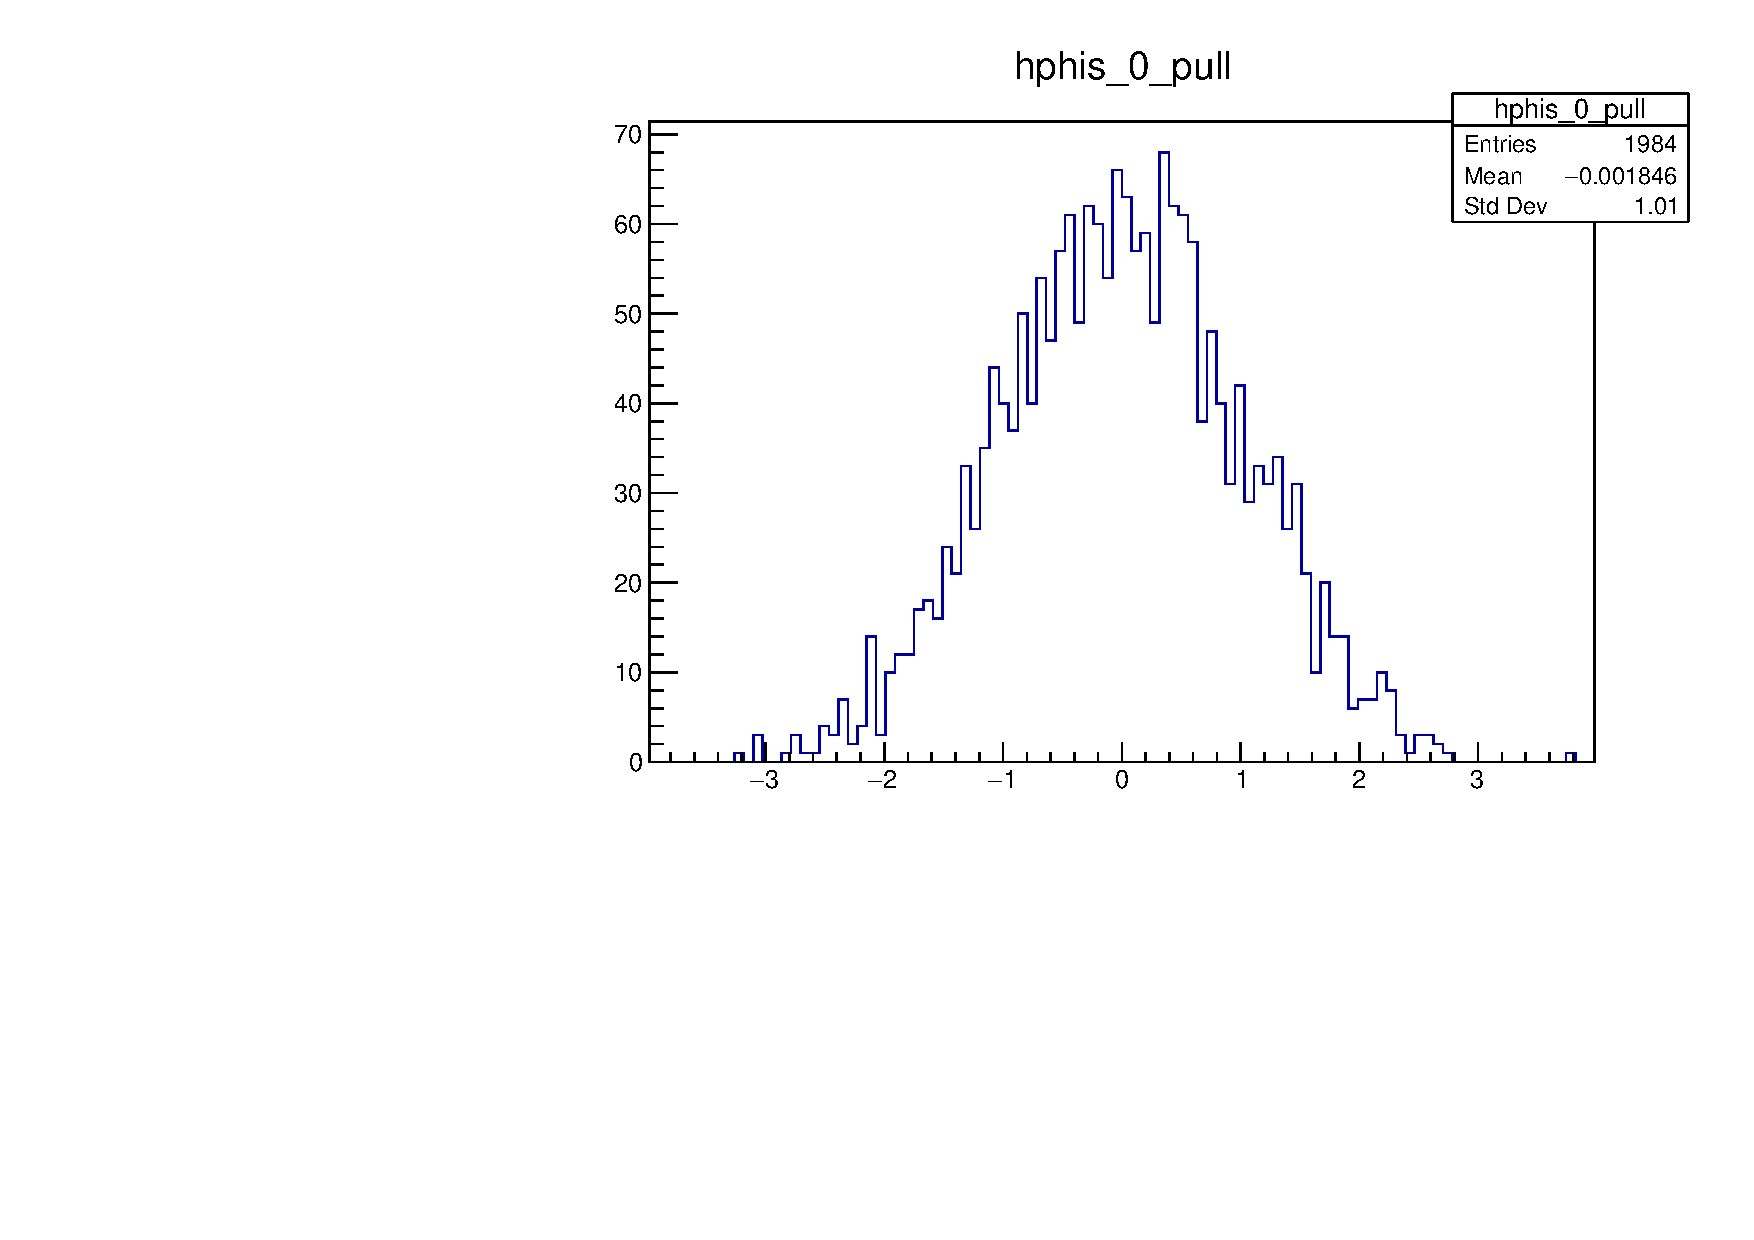
\includegraphics[width=0.3\textwidth]{figs/MCPulls/phis_0_pull.pdf}
	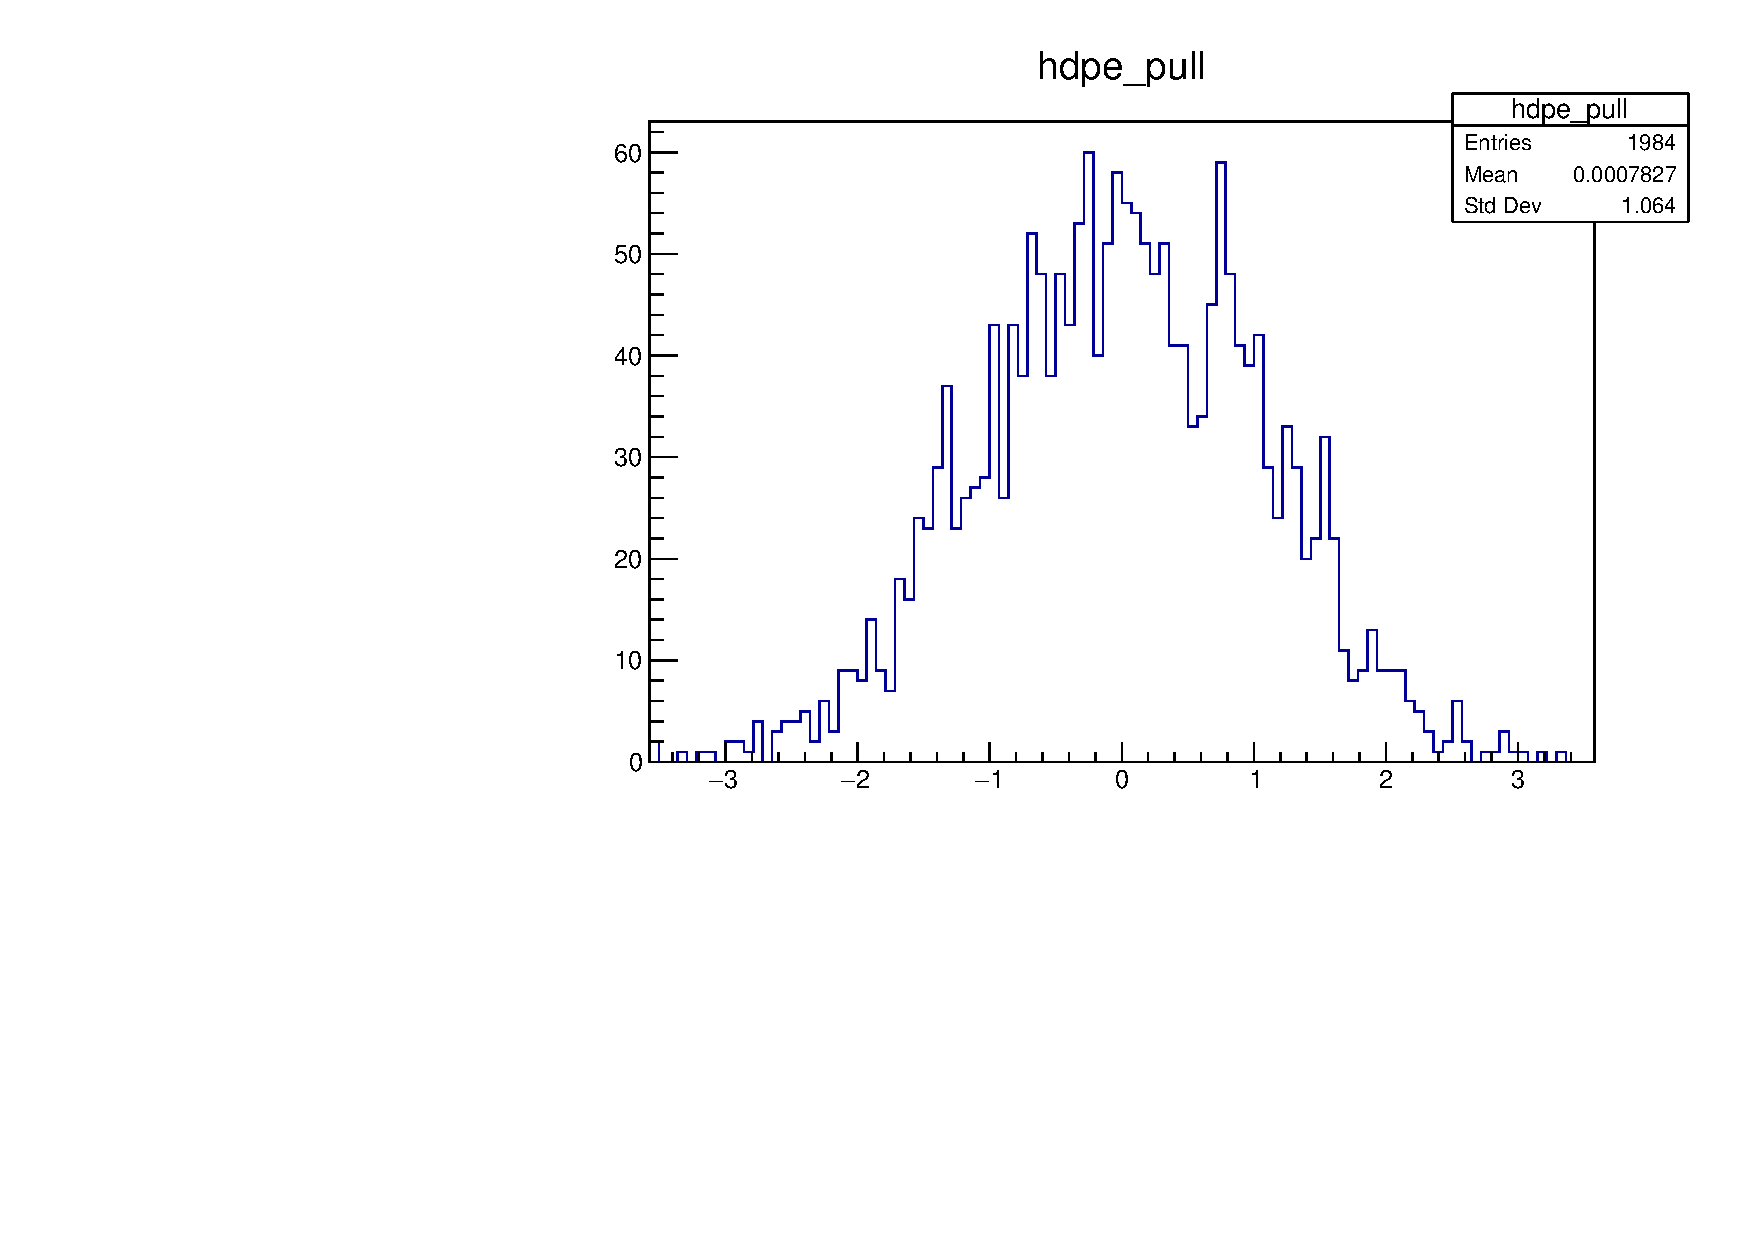
\includegraphics[width=0.3\textwidth]{figs/MCPulls/dpe_pull.pdf}
	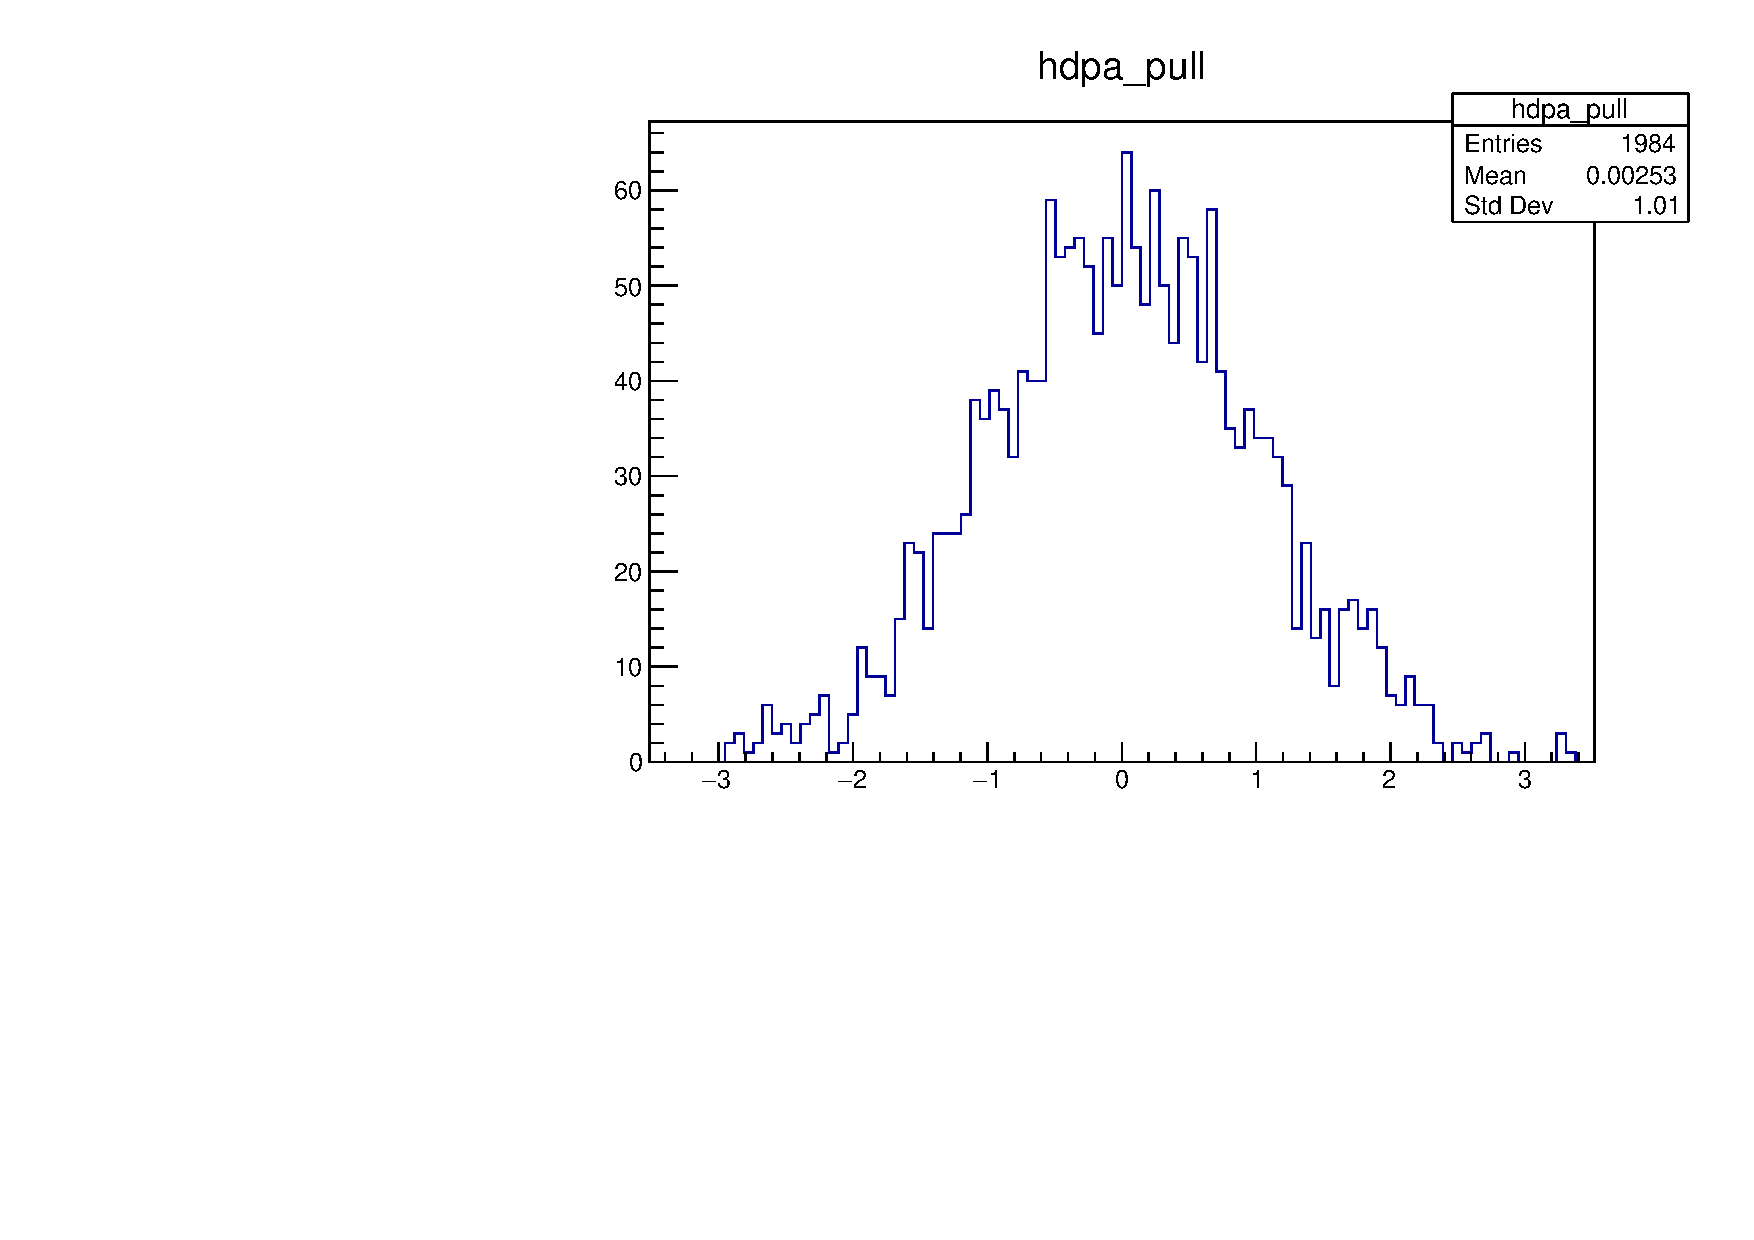
\includegraphics[width=0.3\textwidth]{figs/MCPulls/dpa_pull.pdf}
	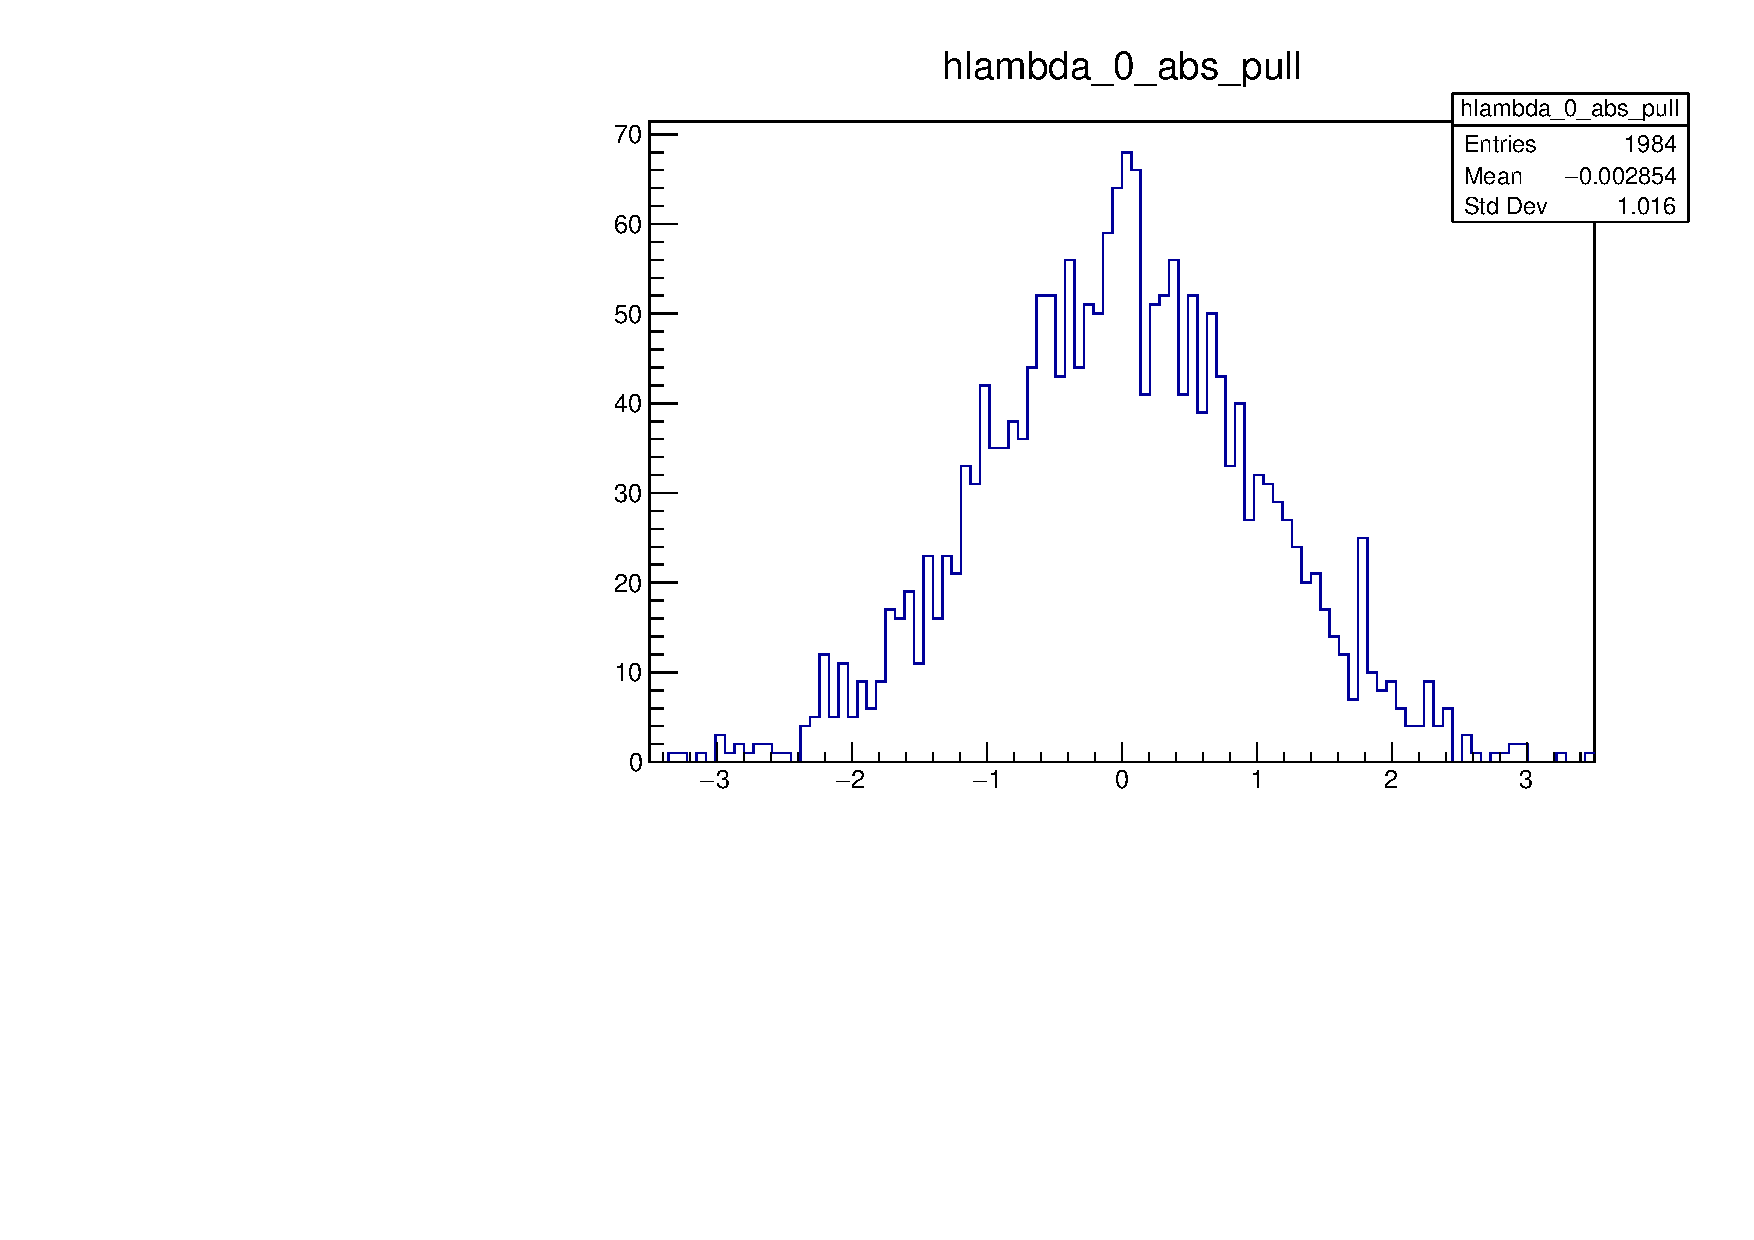
\includegraphics[width=0.3\textwidth]{figs/MCPulls/lambda_0_abs_pull.pdf}
	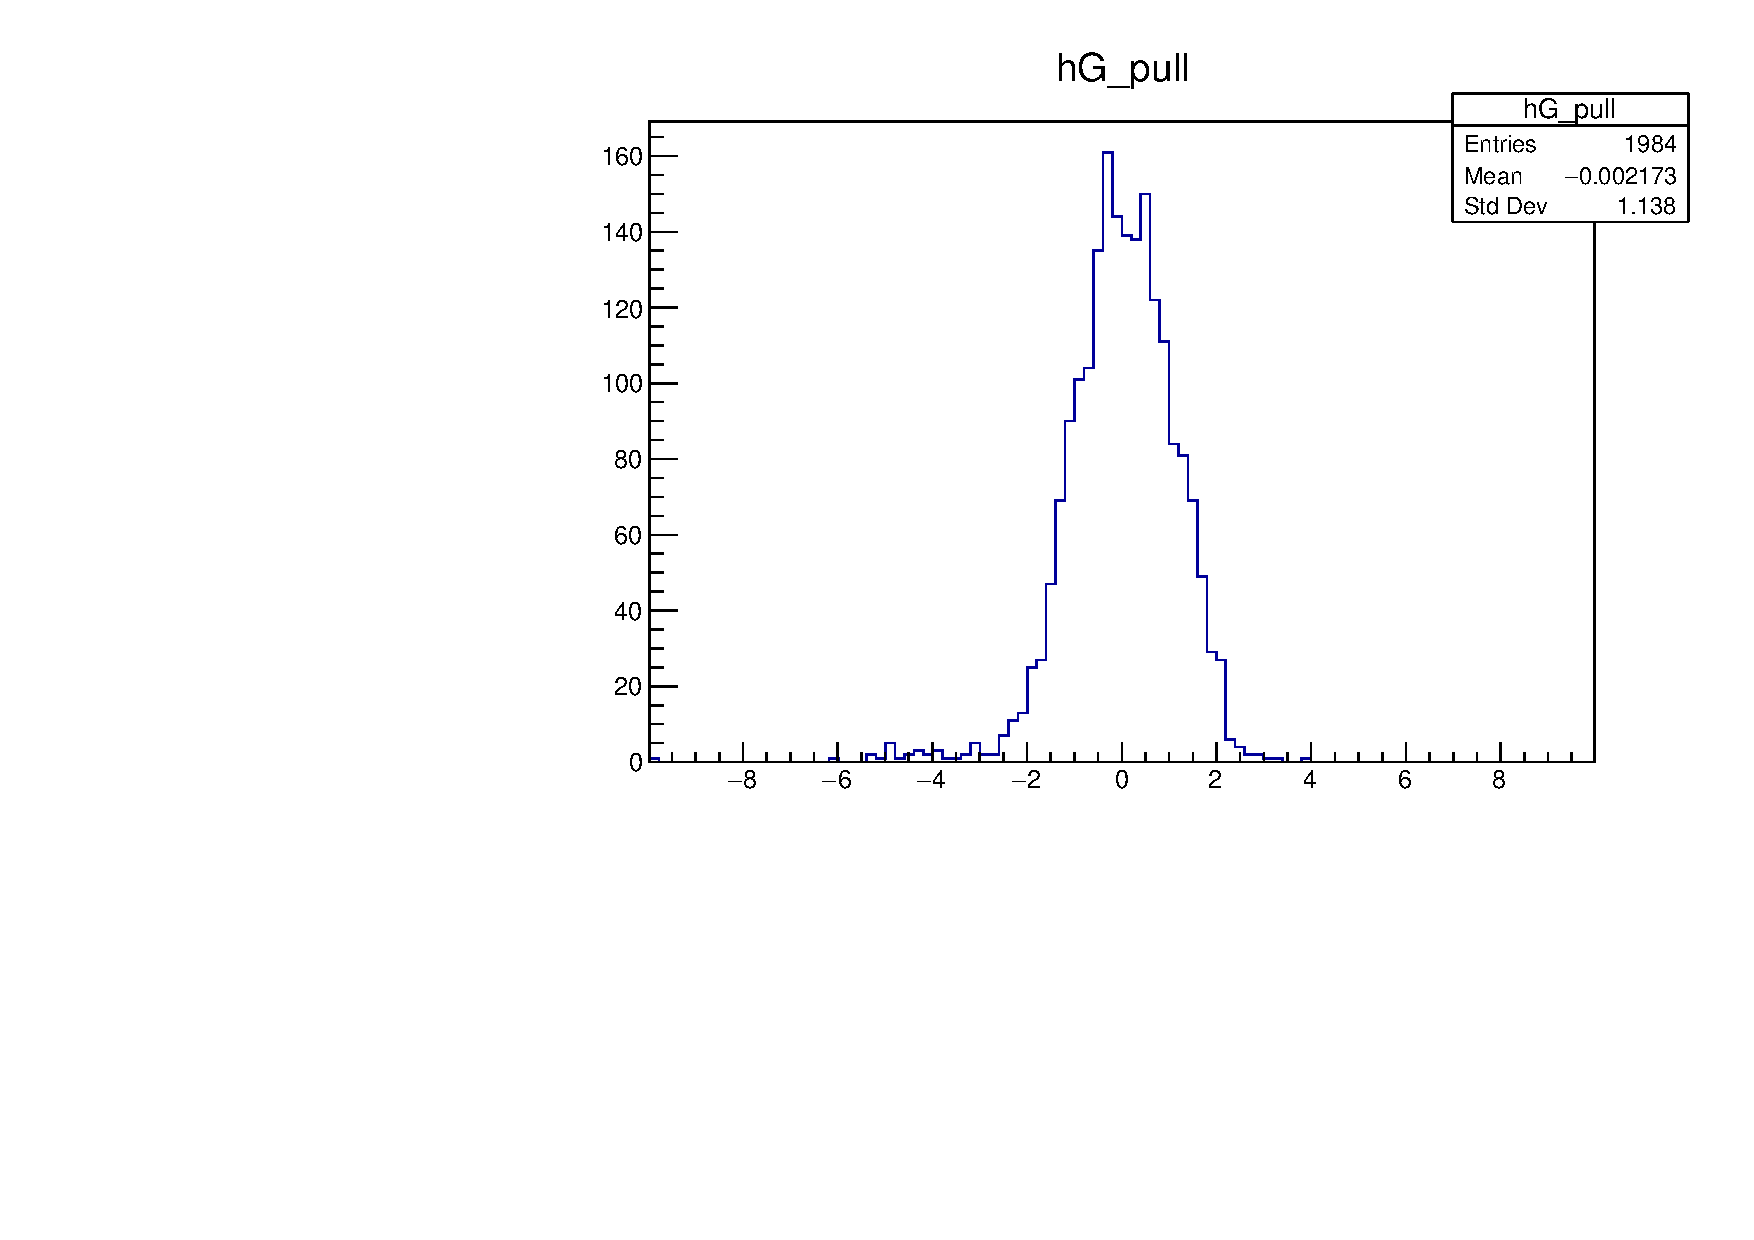
\includegraphics[width=0.3\textwidth]{figs/MCPulls/G_pull.pdf}
	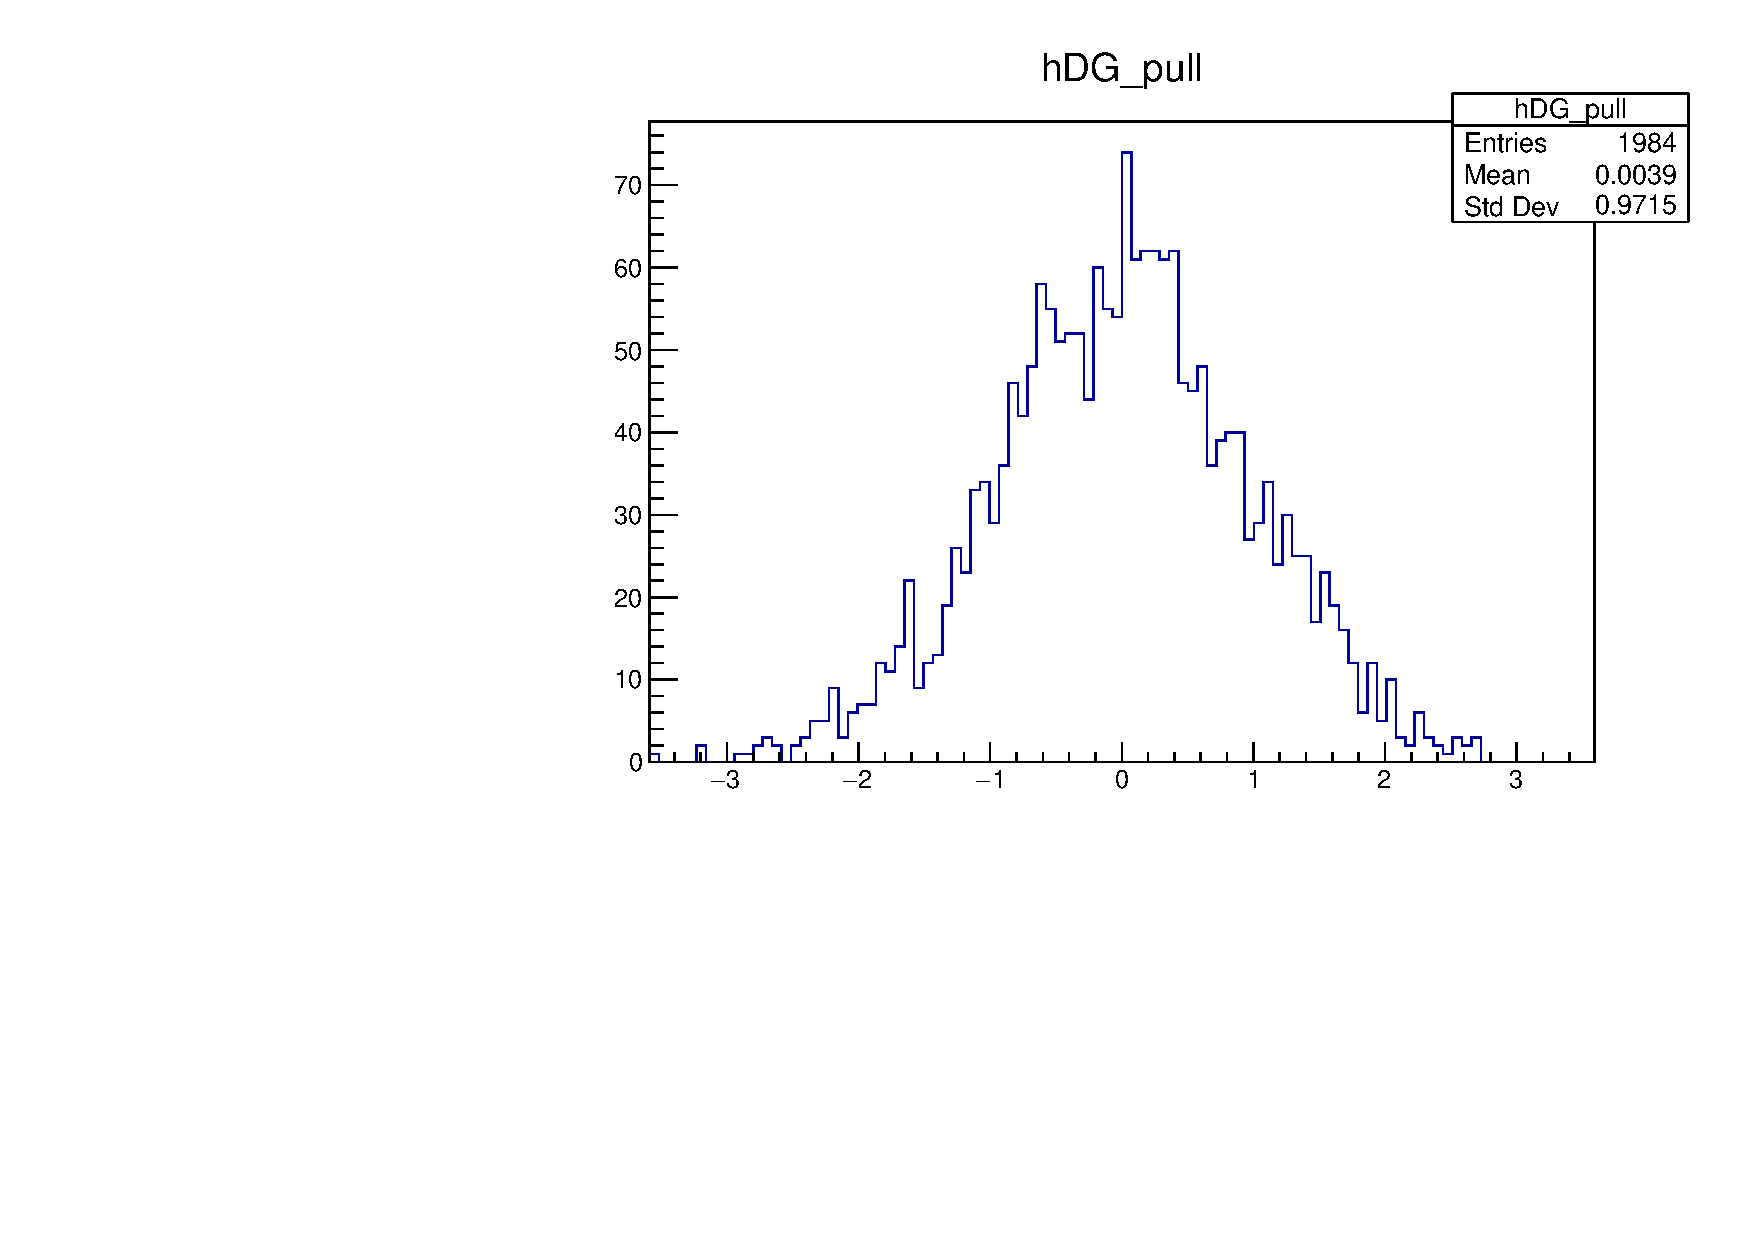
\includegraphics[width=0.3\textwidth]{figs/MCPulls/DG_pull.pdf}
	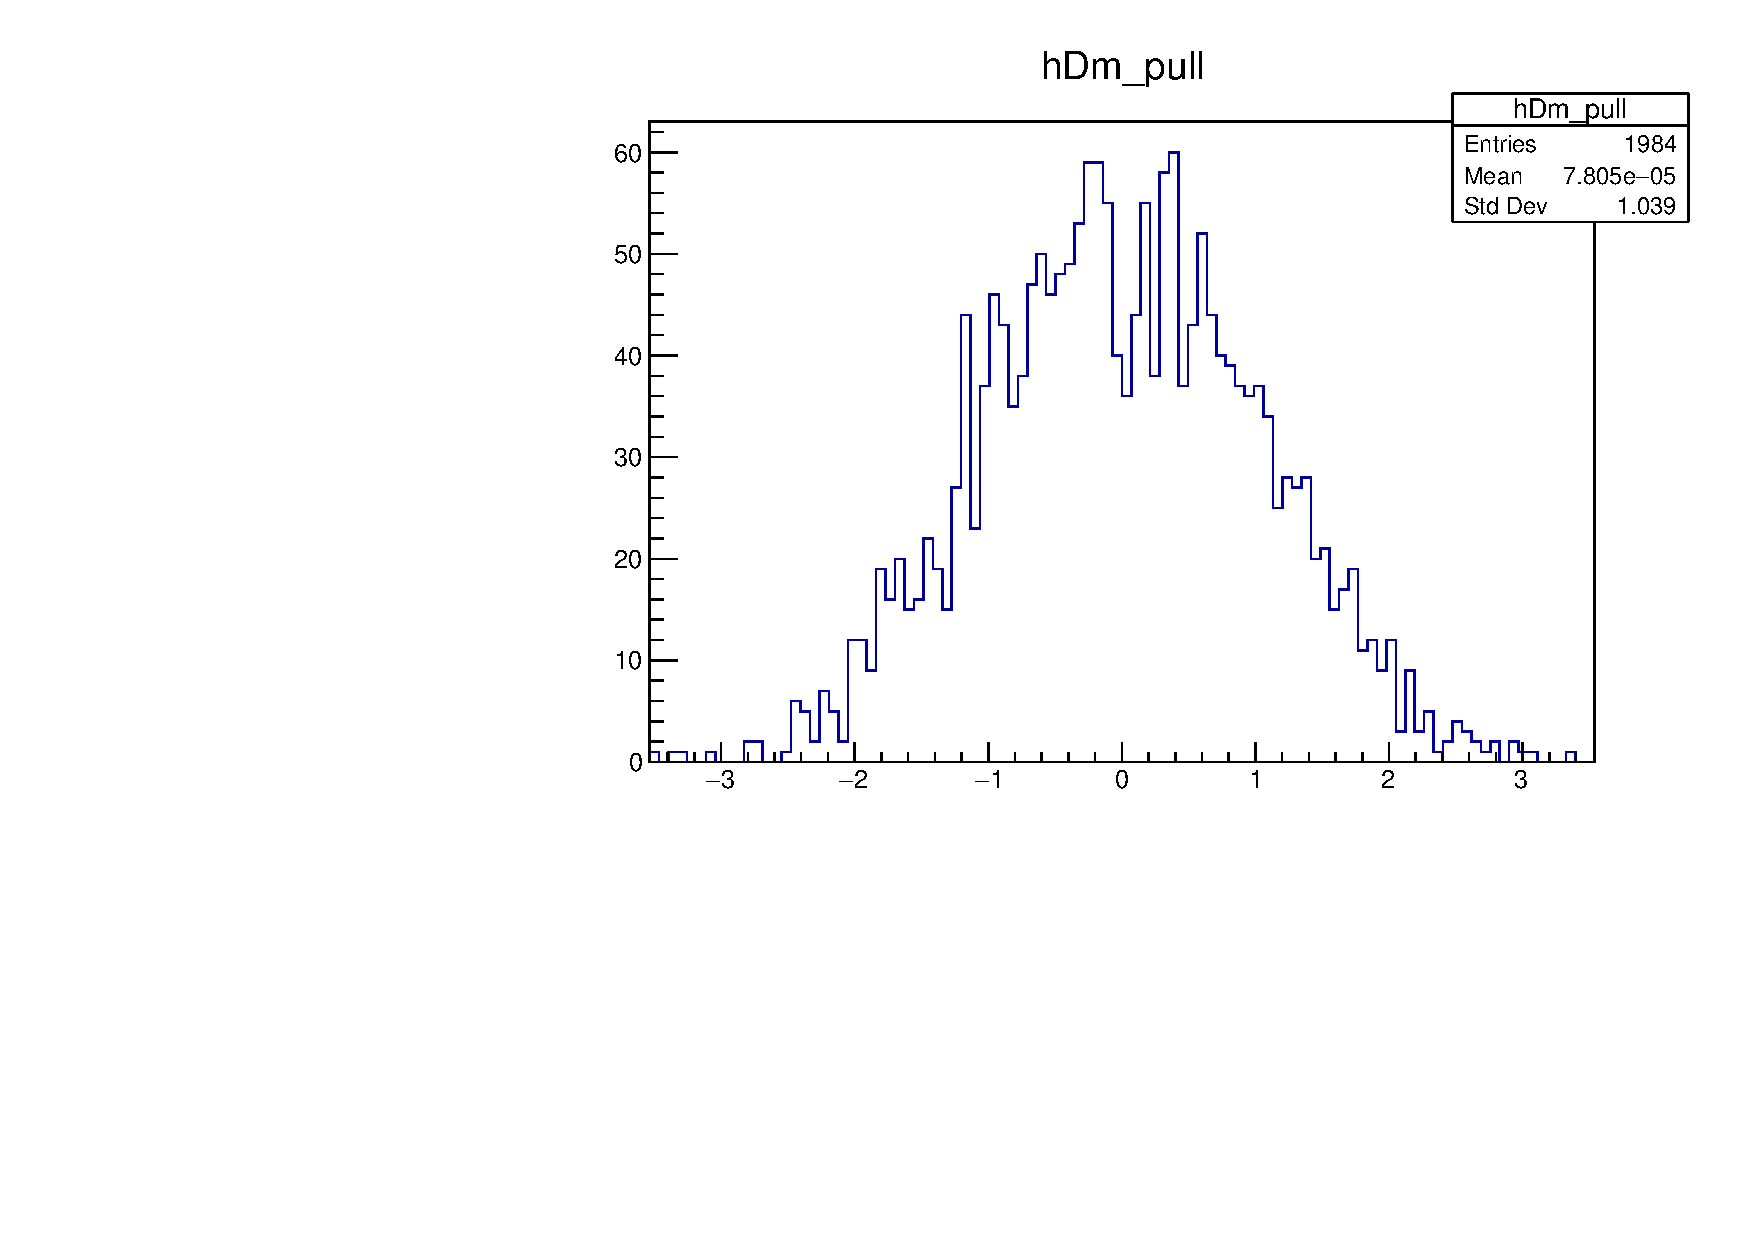
\includegraphics[width=0.3\textwidth]{figs/MCPulls/Dm_pull.pdf}
   \end{center}
   \caption{
       Pull distributions of the fit parameters using bootstrapping (MC).
       Pulls are computed relative to MC generation values.
   }
   \label{fig:Pulls_MC}
\end{figure}

\begin{figure}[tb]
   \begin{center}
	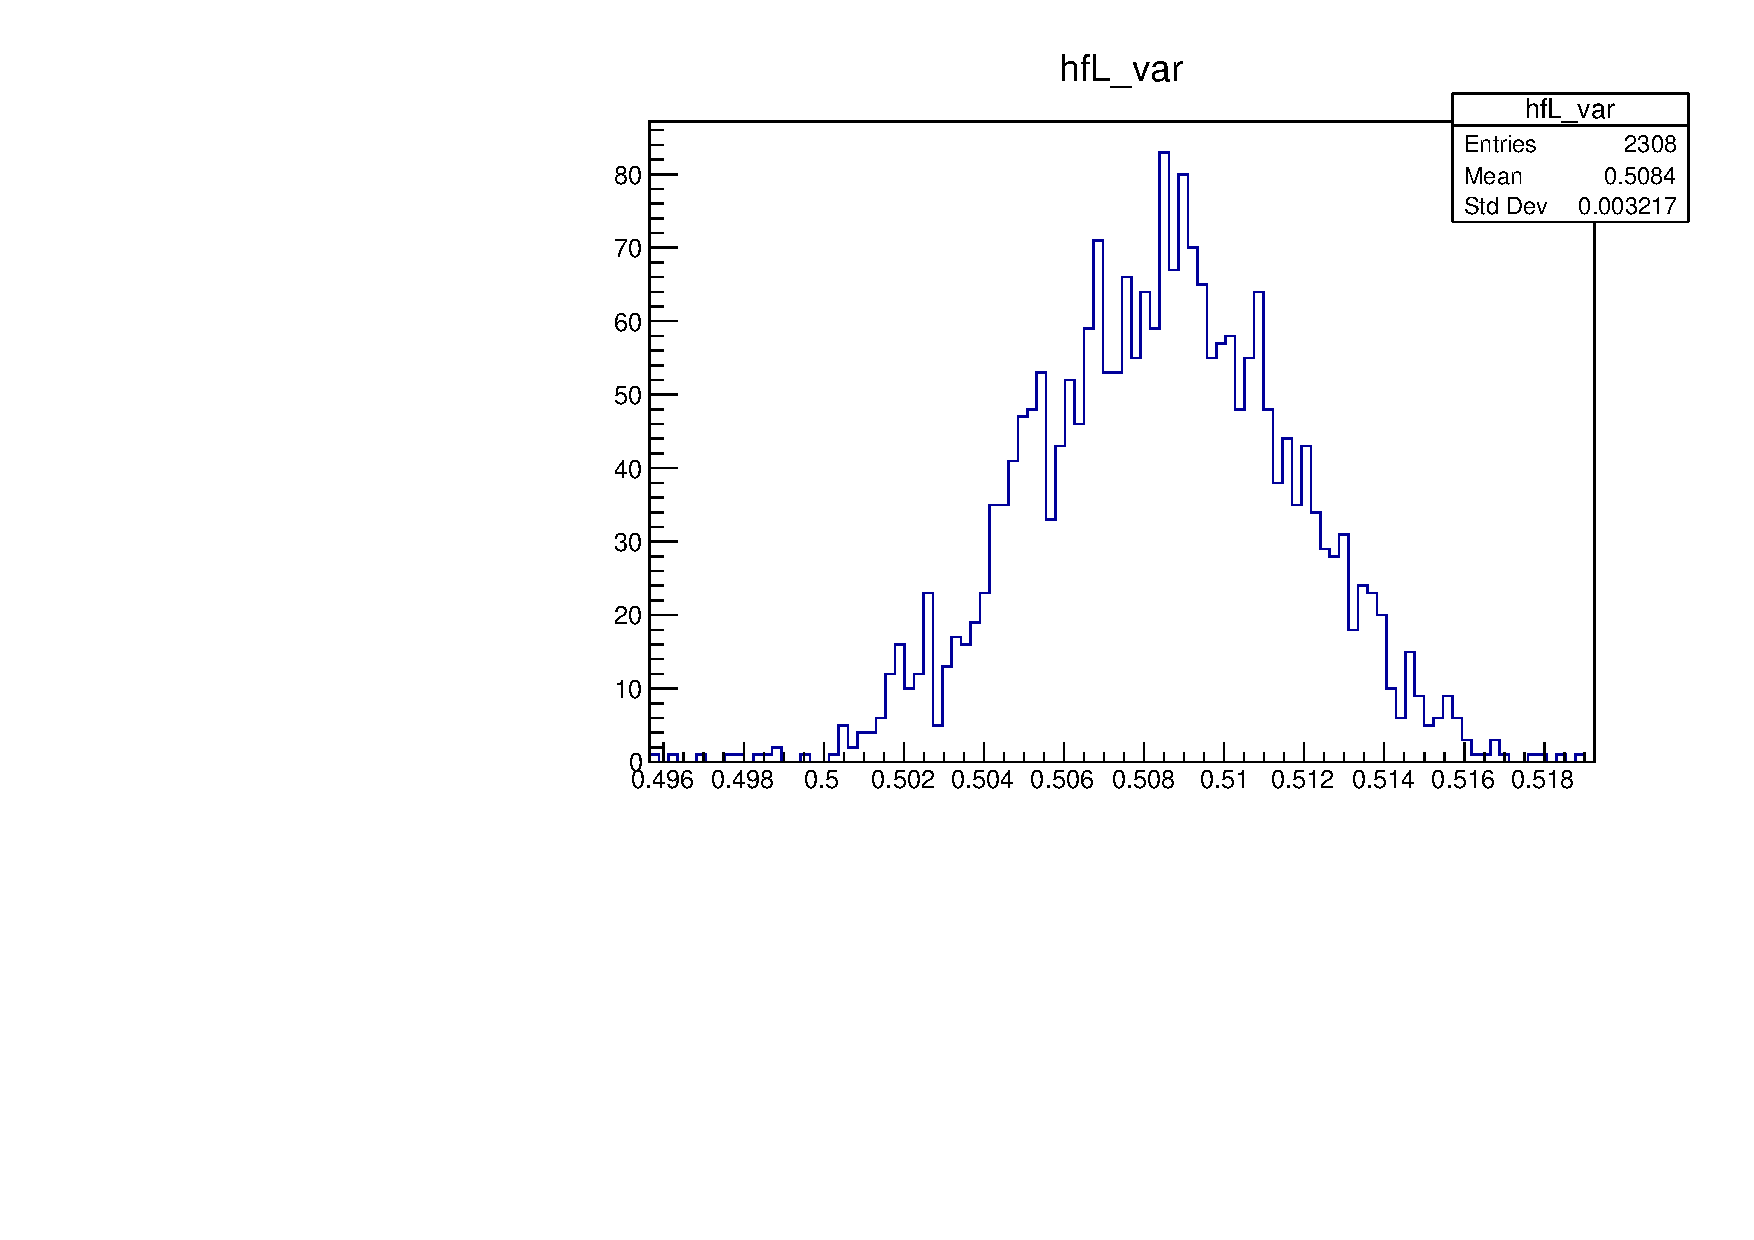
\includegraphics[width=0.3\textwidth]{figs/DataVars/fL_var.pdf}
	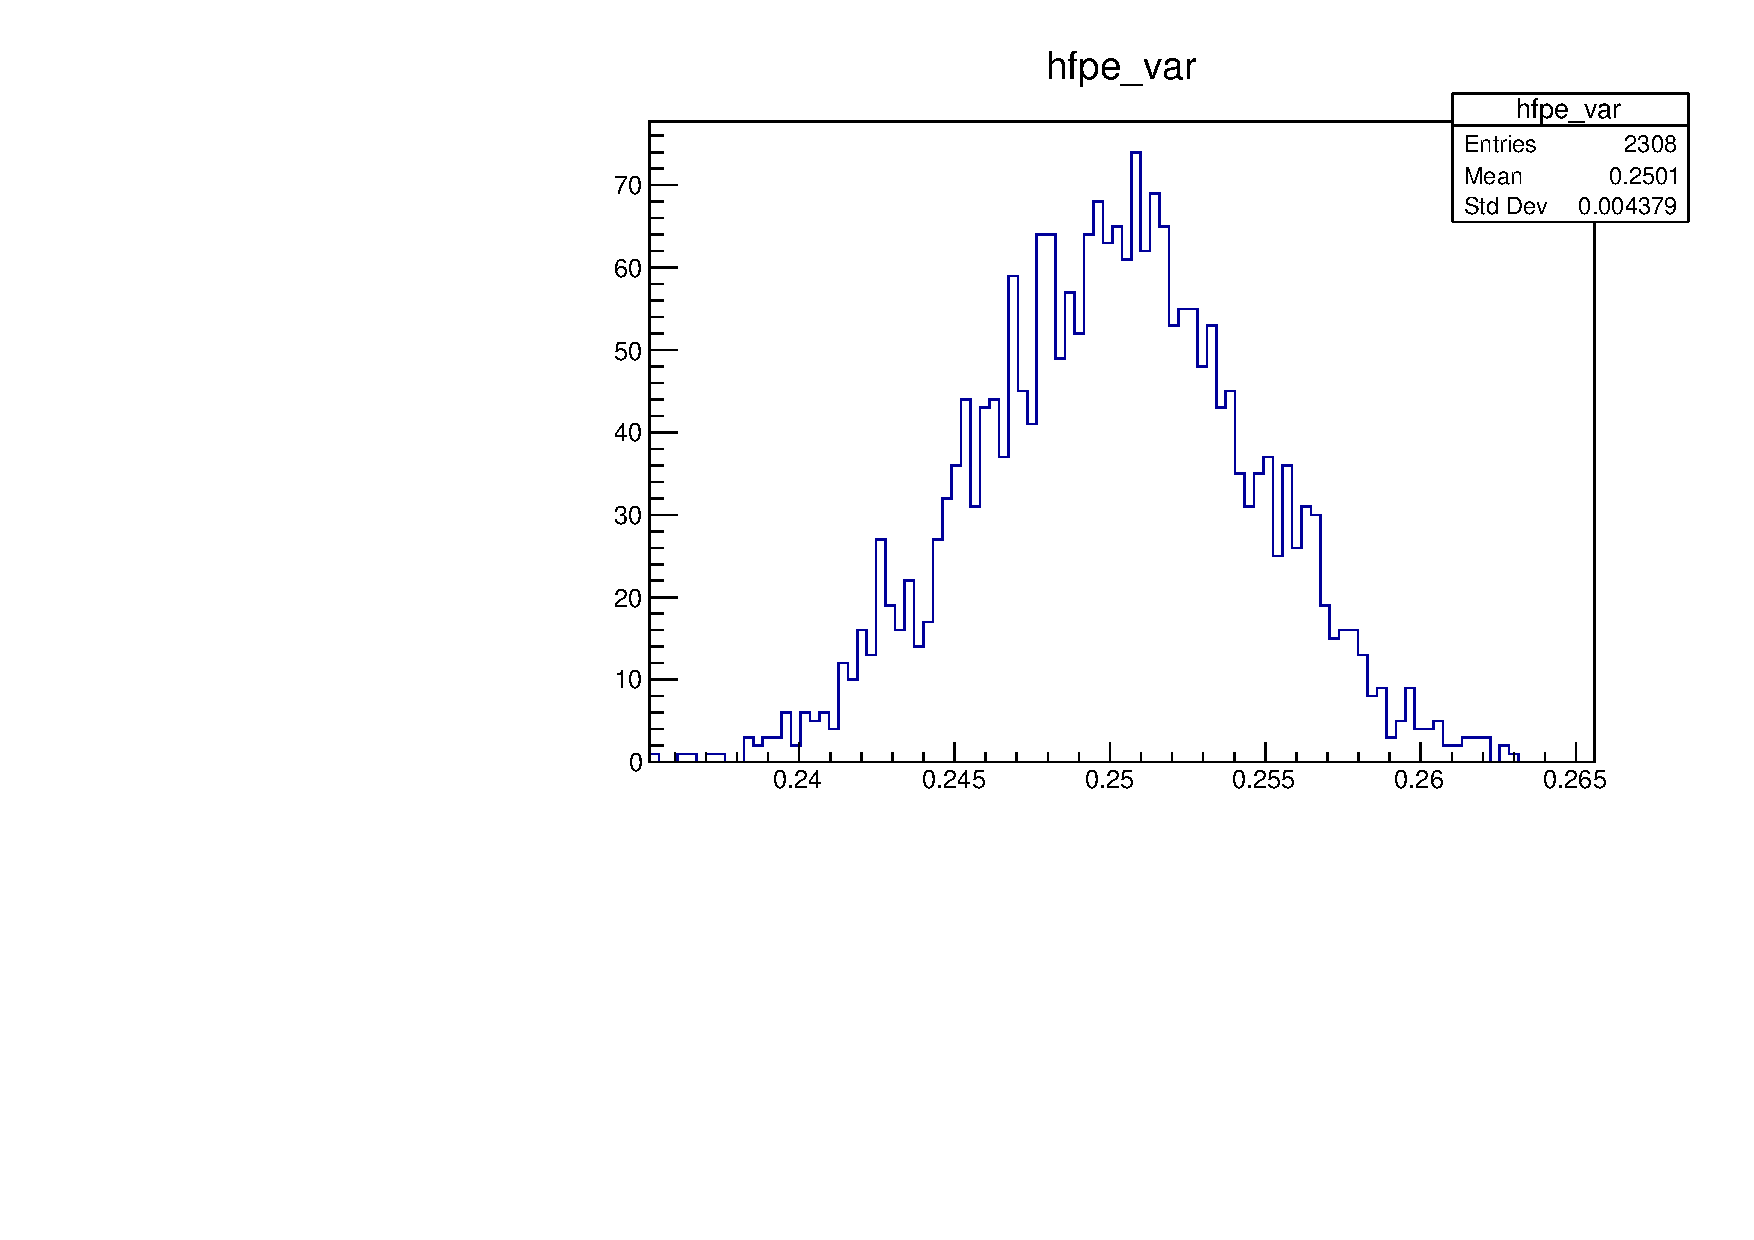
\includegraphics[width=0.3\textwidth]{figs/DataVars/fpe_var.pdf}
	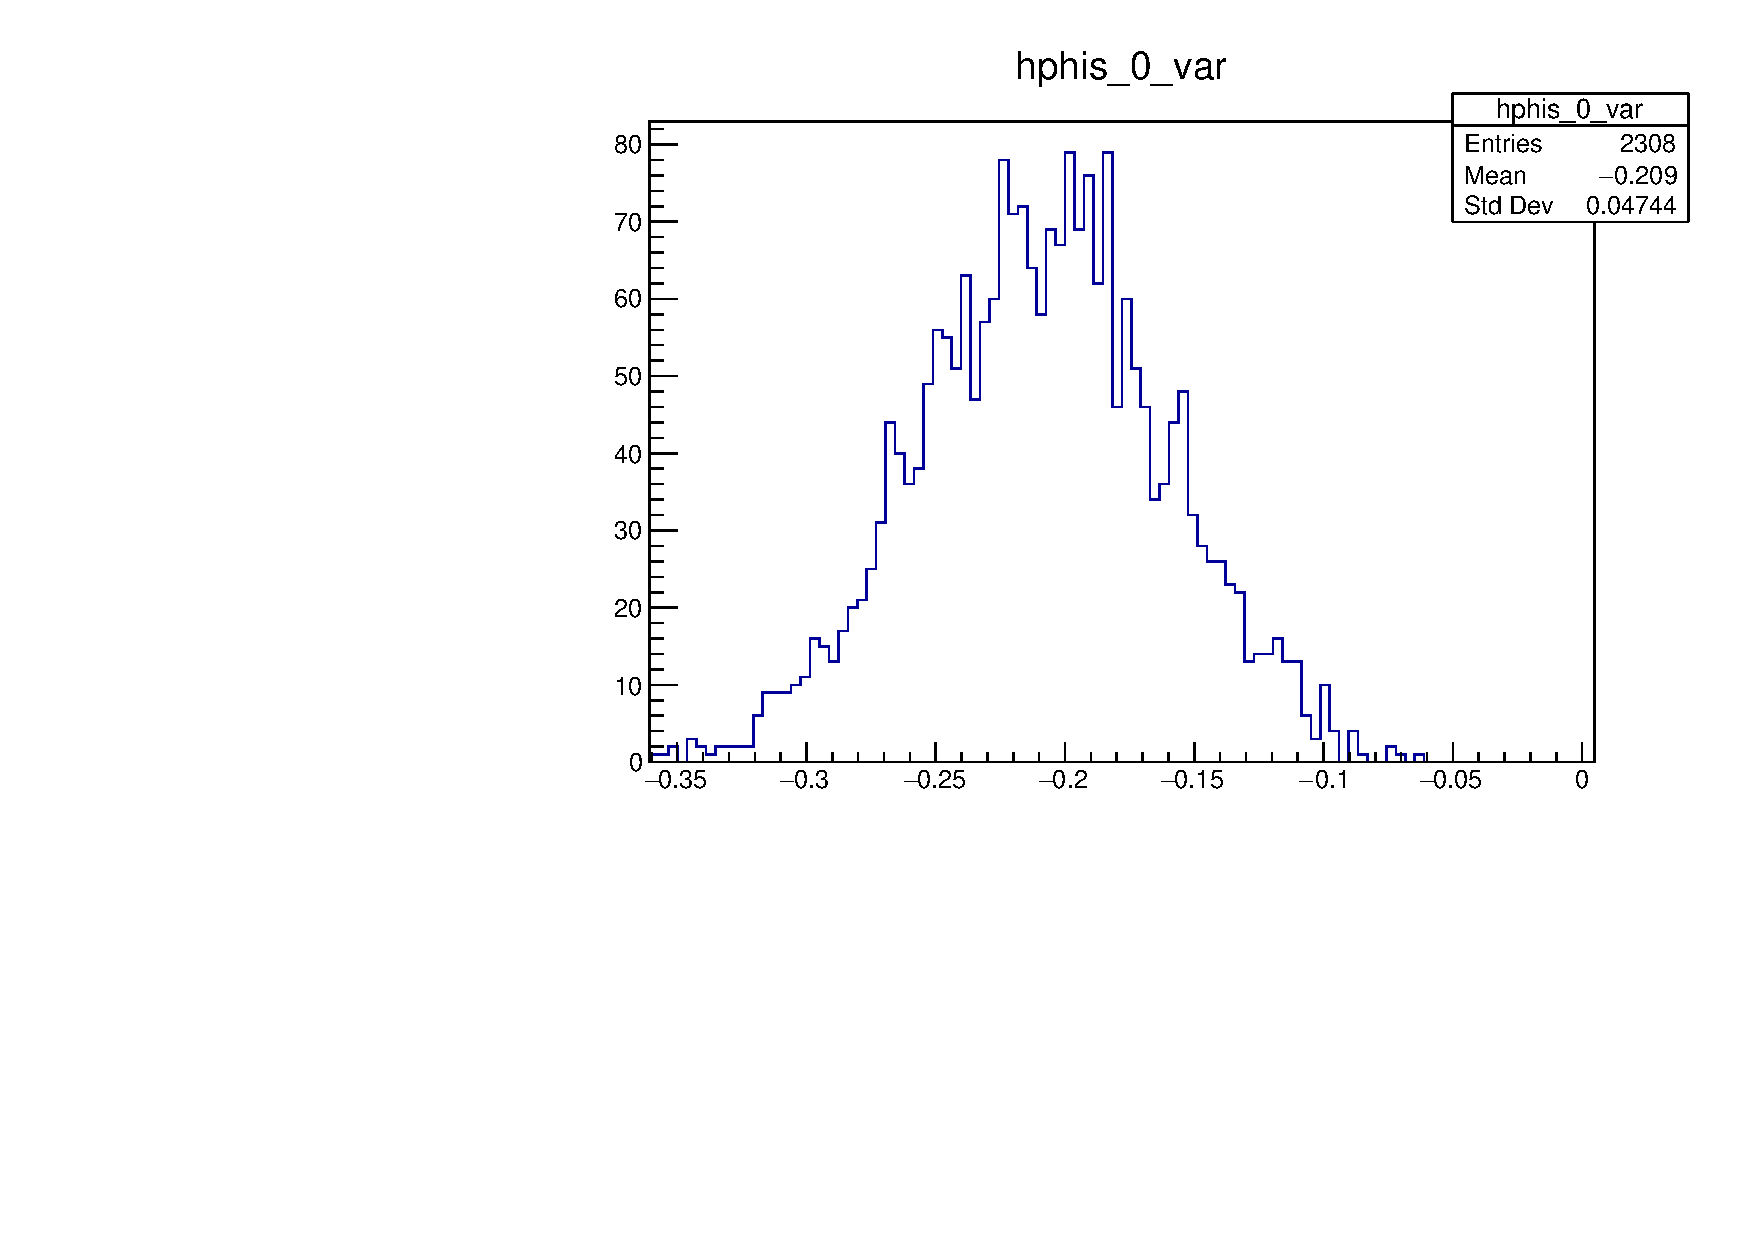
\includegraphics[width=0.3\textwidth]{figs/DataVars/phis_0_var.pdf}
	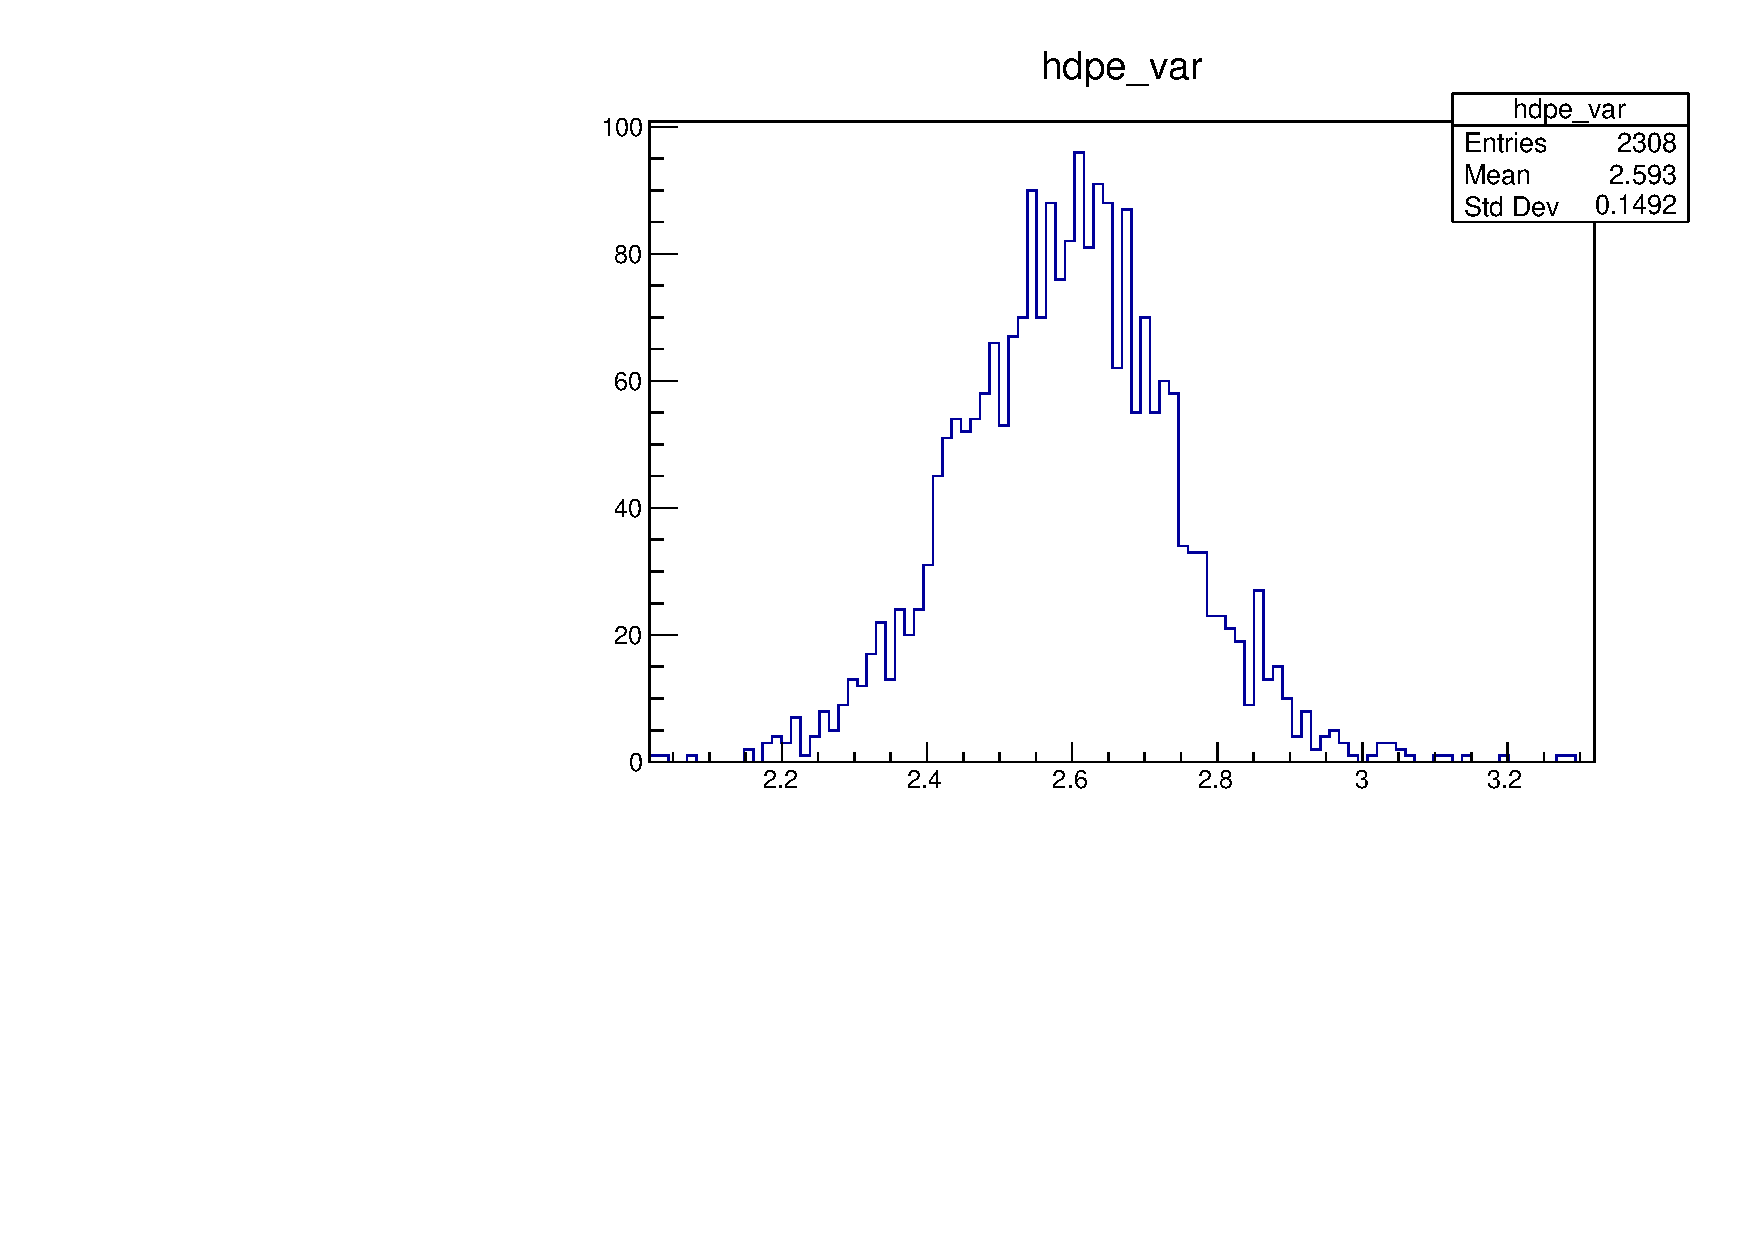
\includegraphics[width=0.3\textwidth]{figs/DataVars/dpe_var.pdf}
	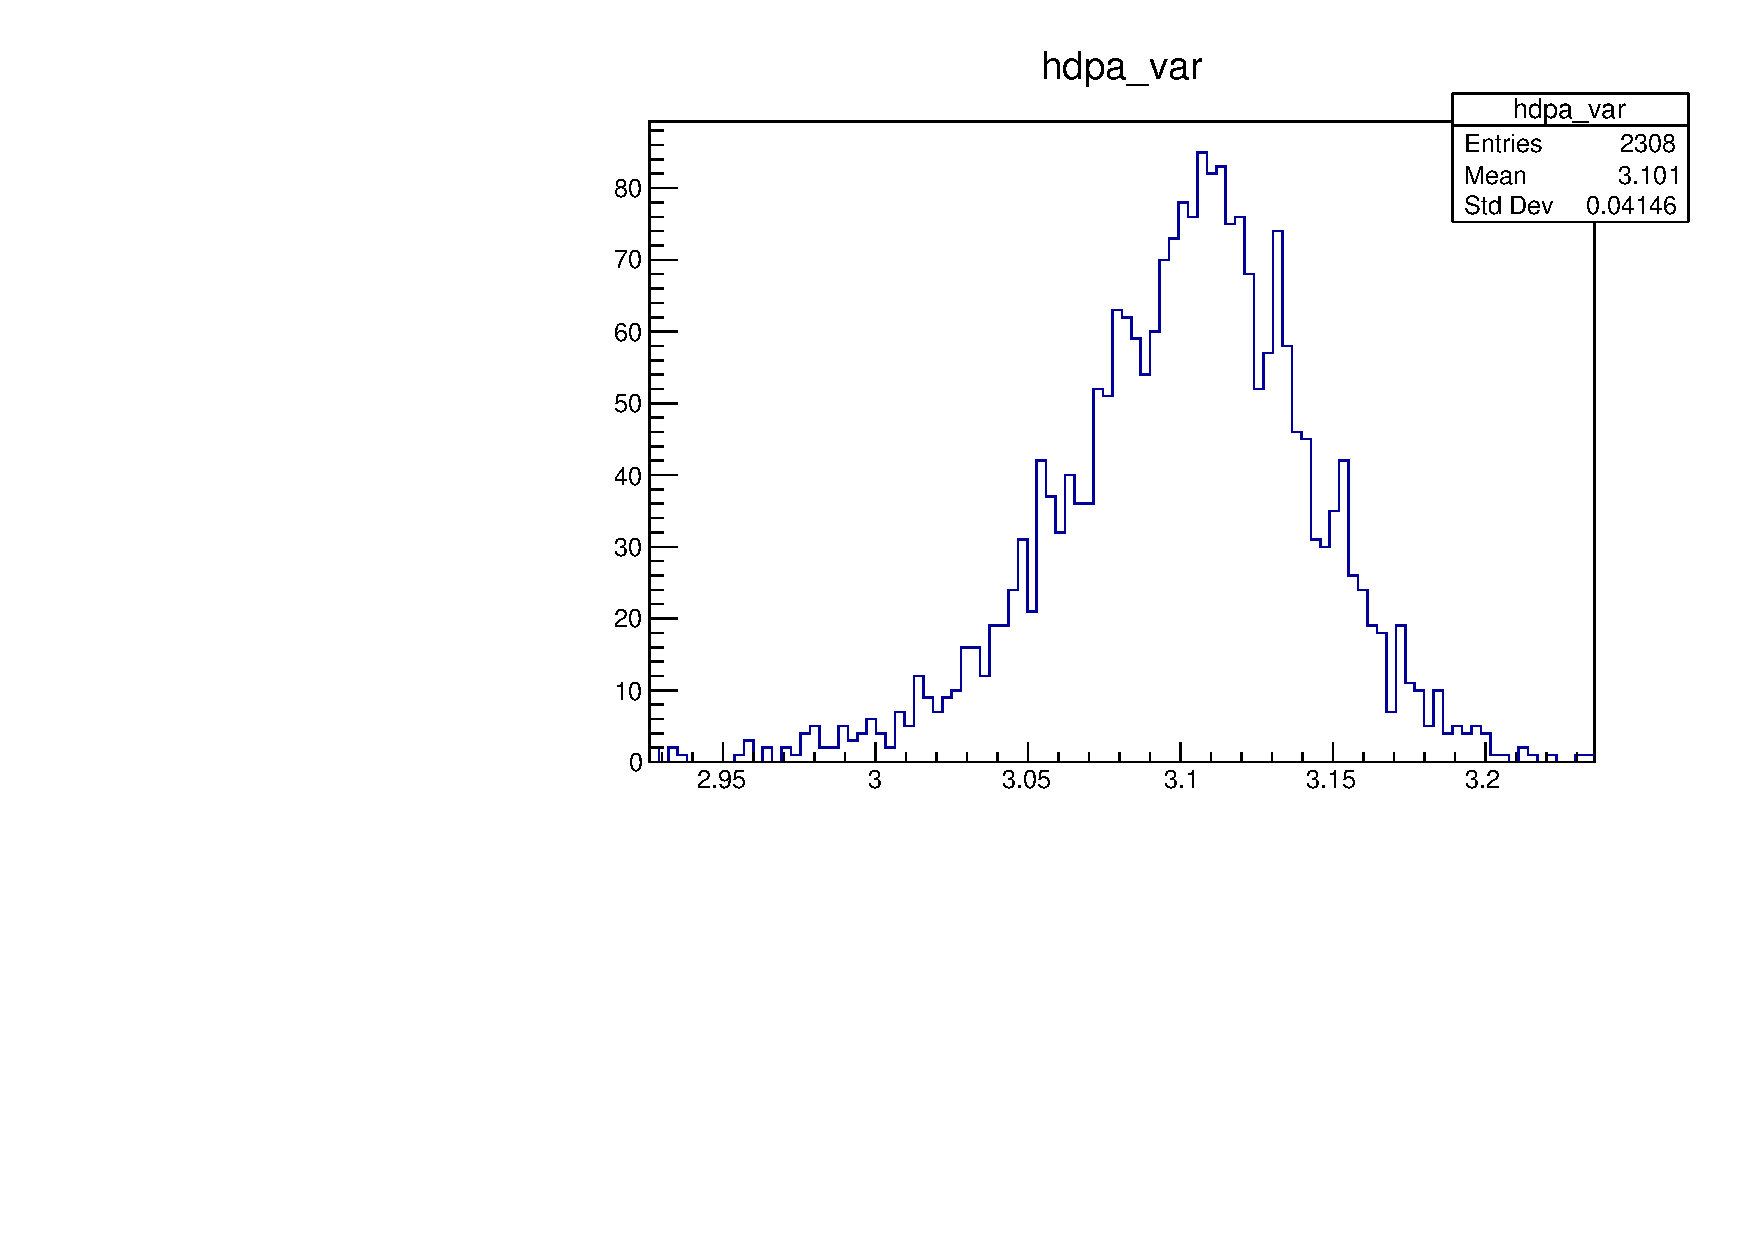
\includegraphics[width=0.3\textwidth]{figs/DataVars/dpa_var.pdf}
	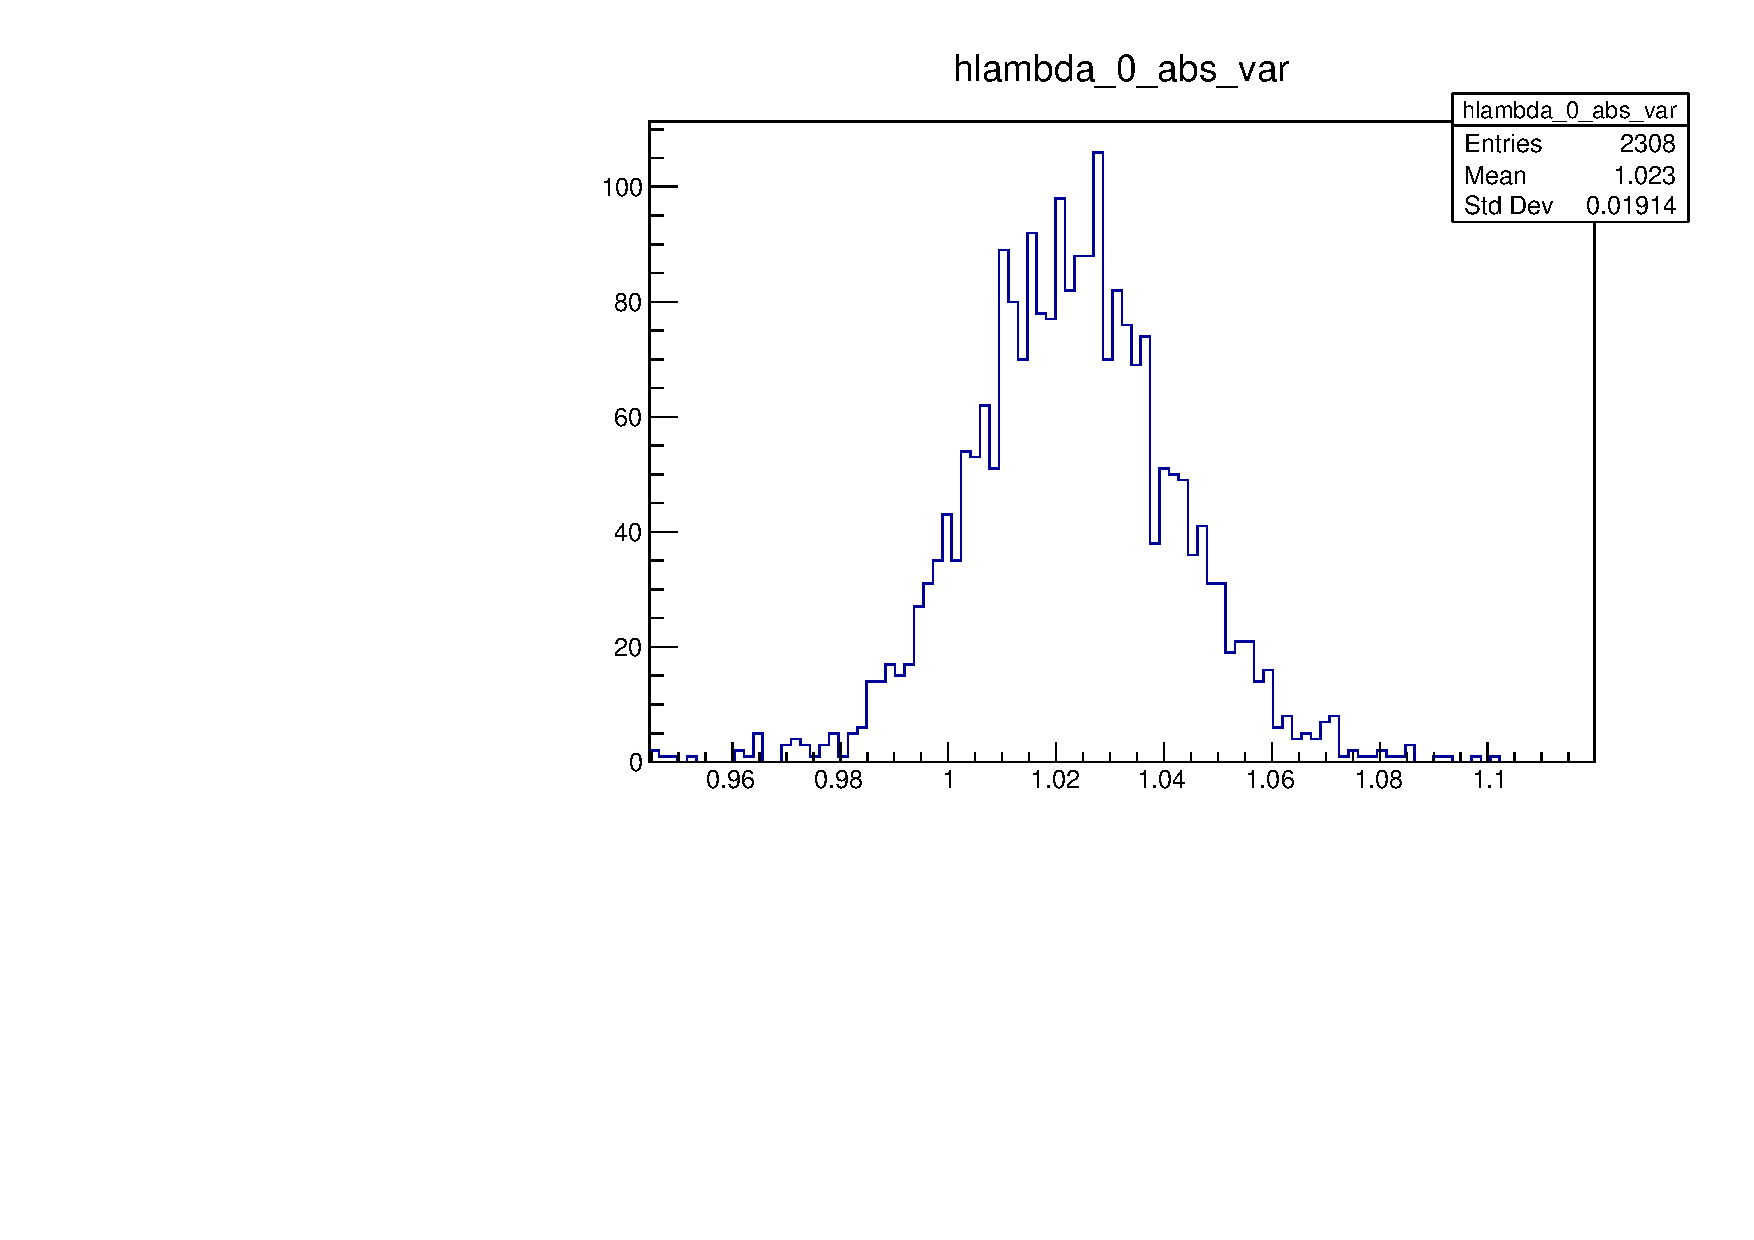
\includegraphics[width=0.3\textwidth]{figs/DataVars/lambda_0_abs_var.pdf}
	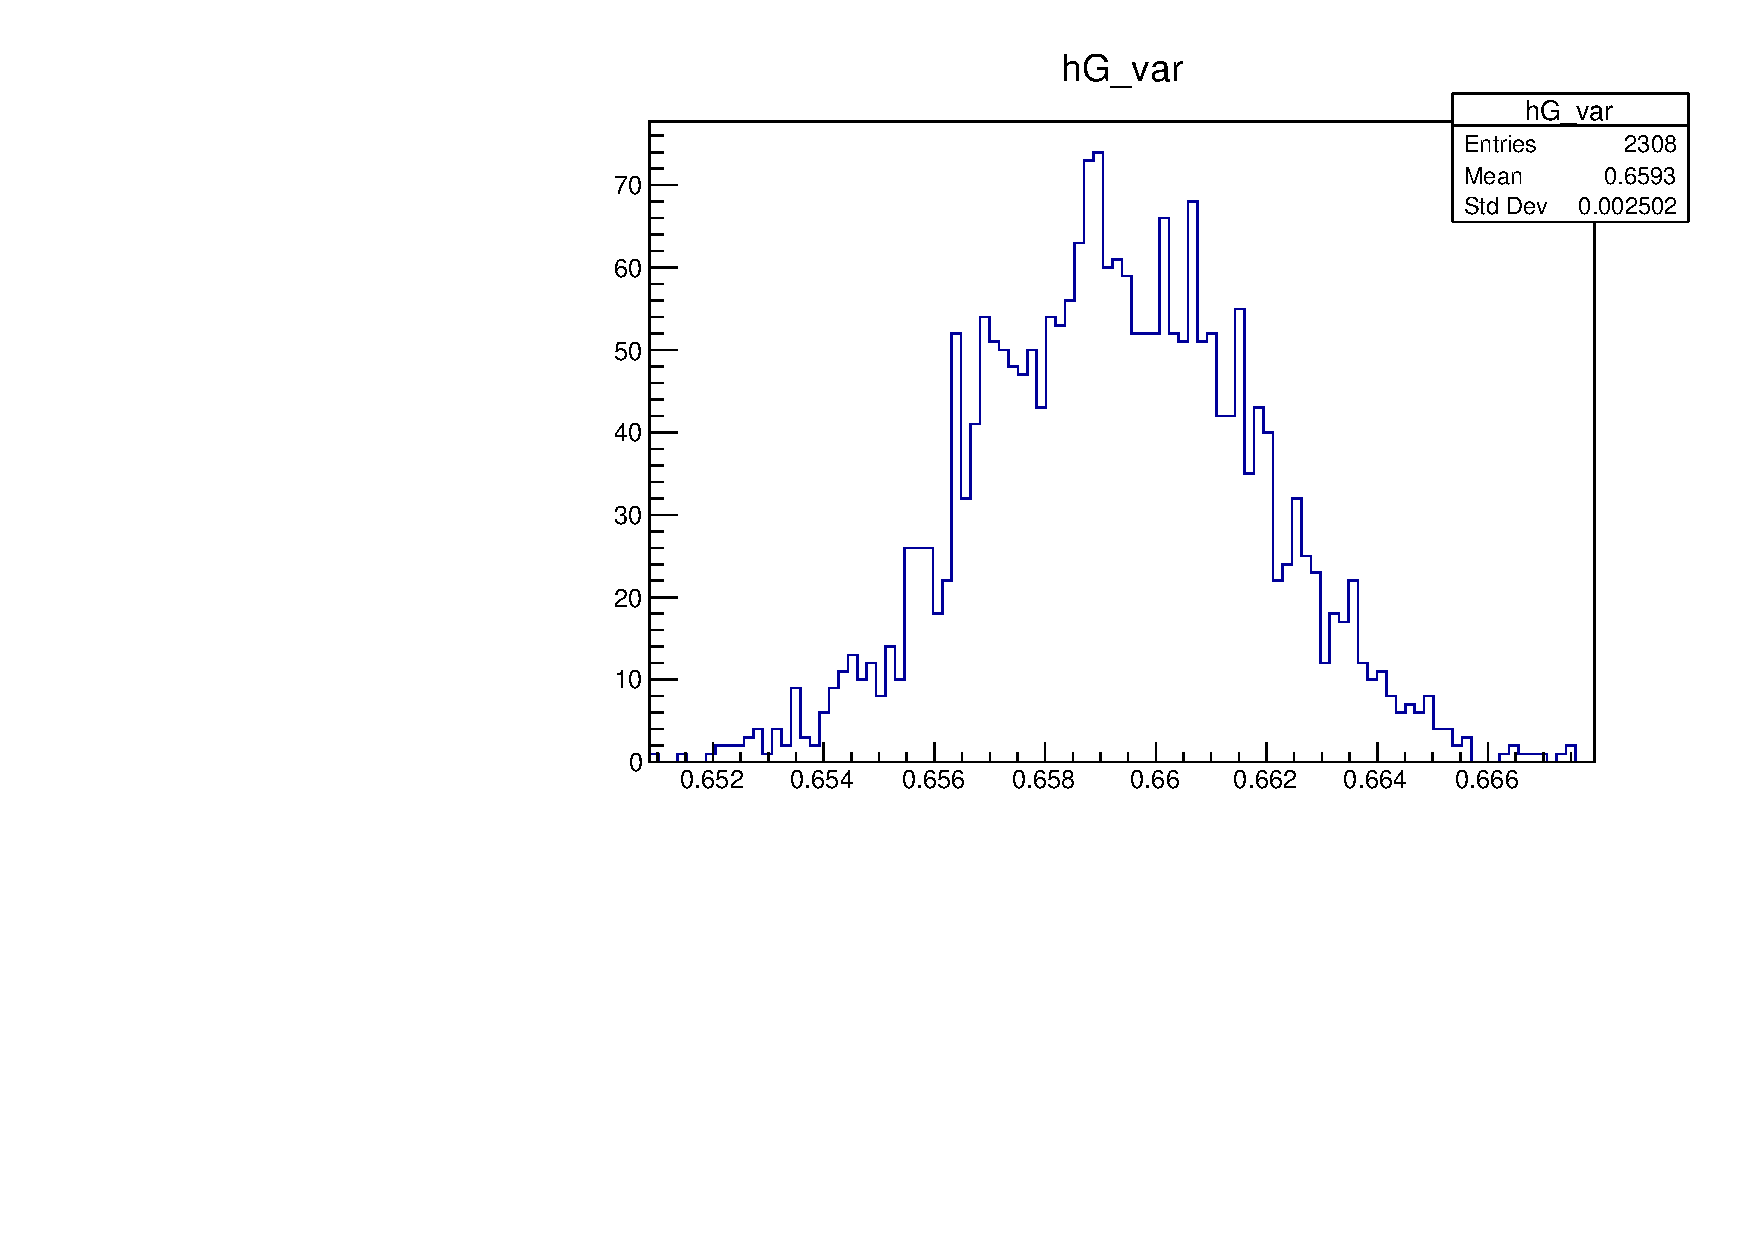
\includegraphics[width=0.3\textwidth]{figs/DataVars/G_var.pdf}
	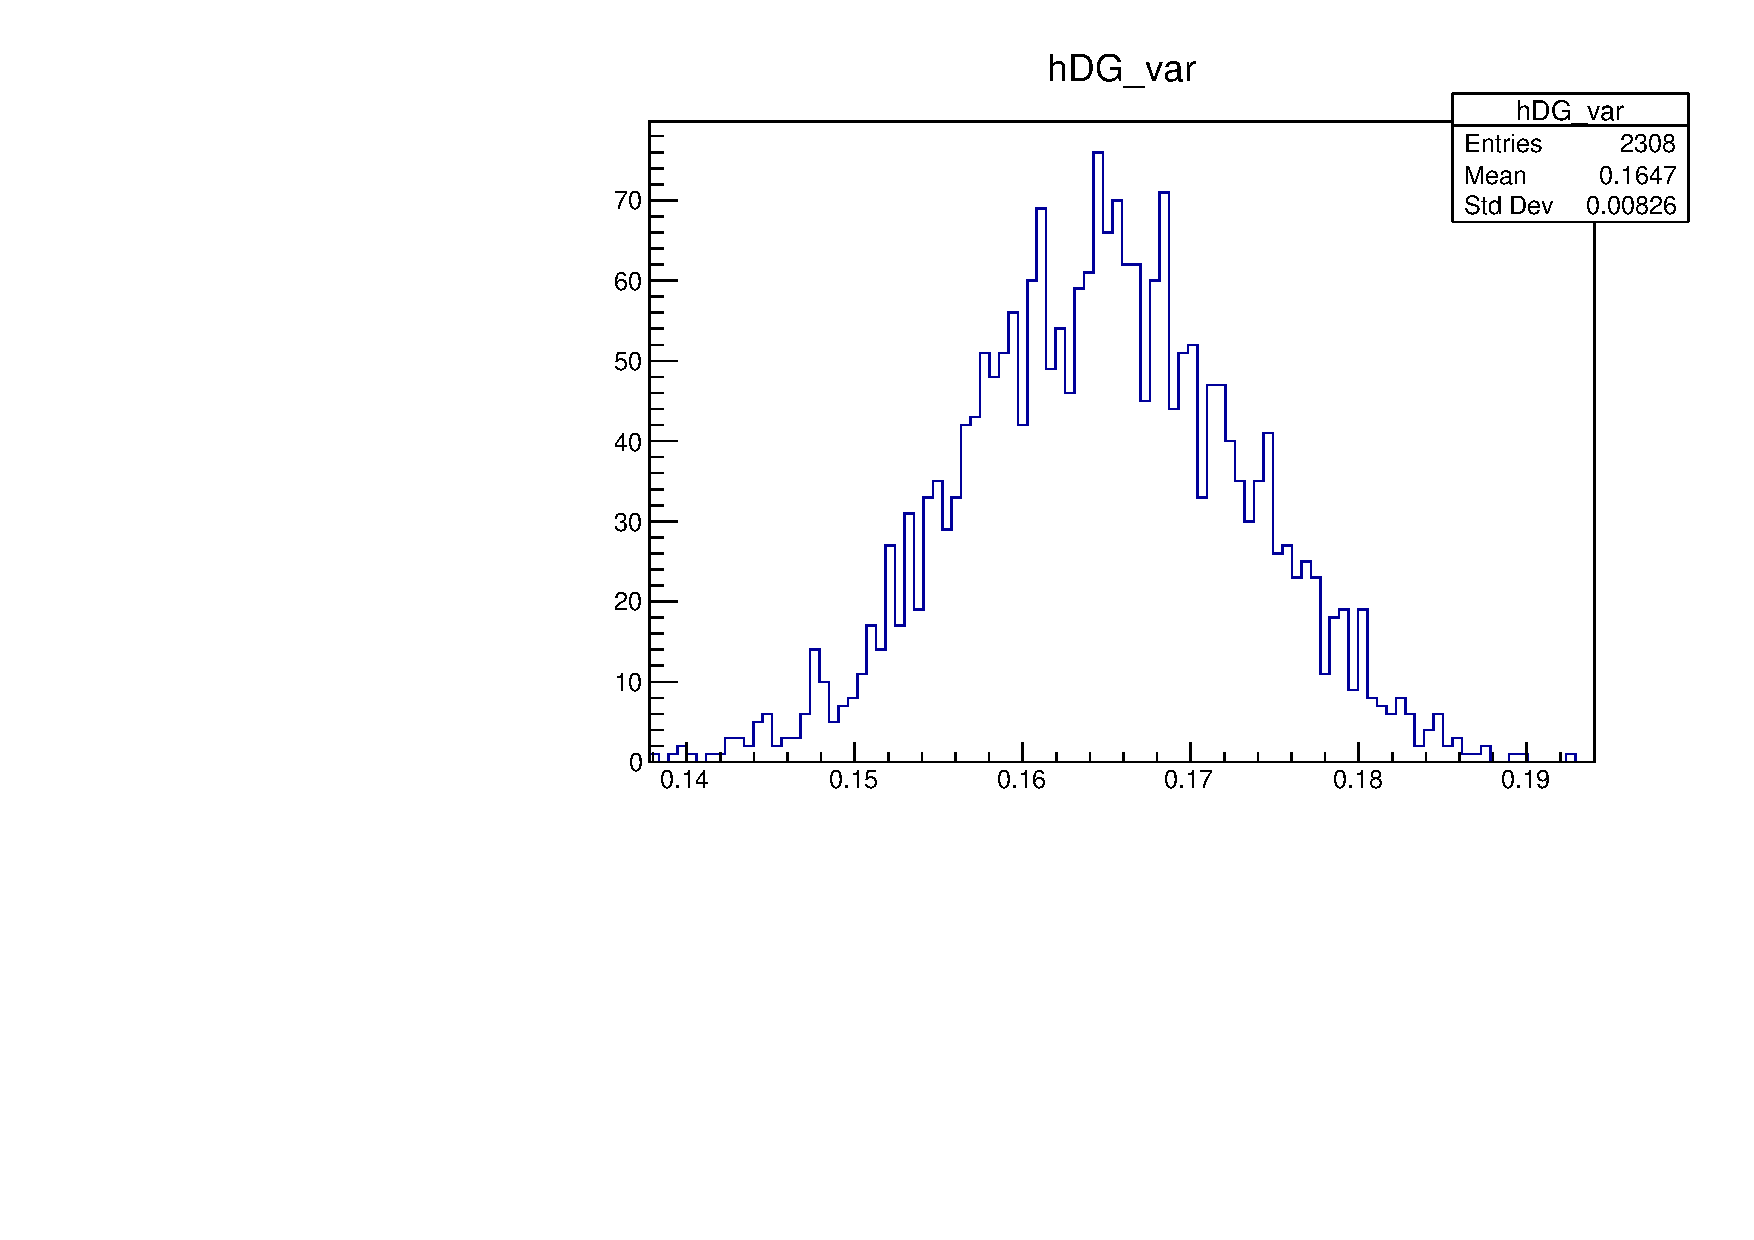
\includegraphics[width=0.3\textwidth]{figs/DataVars/DG_var.pdf}
	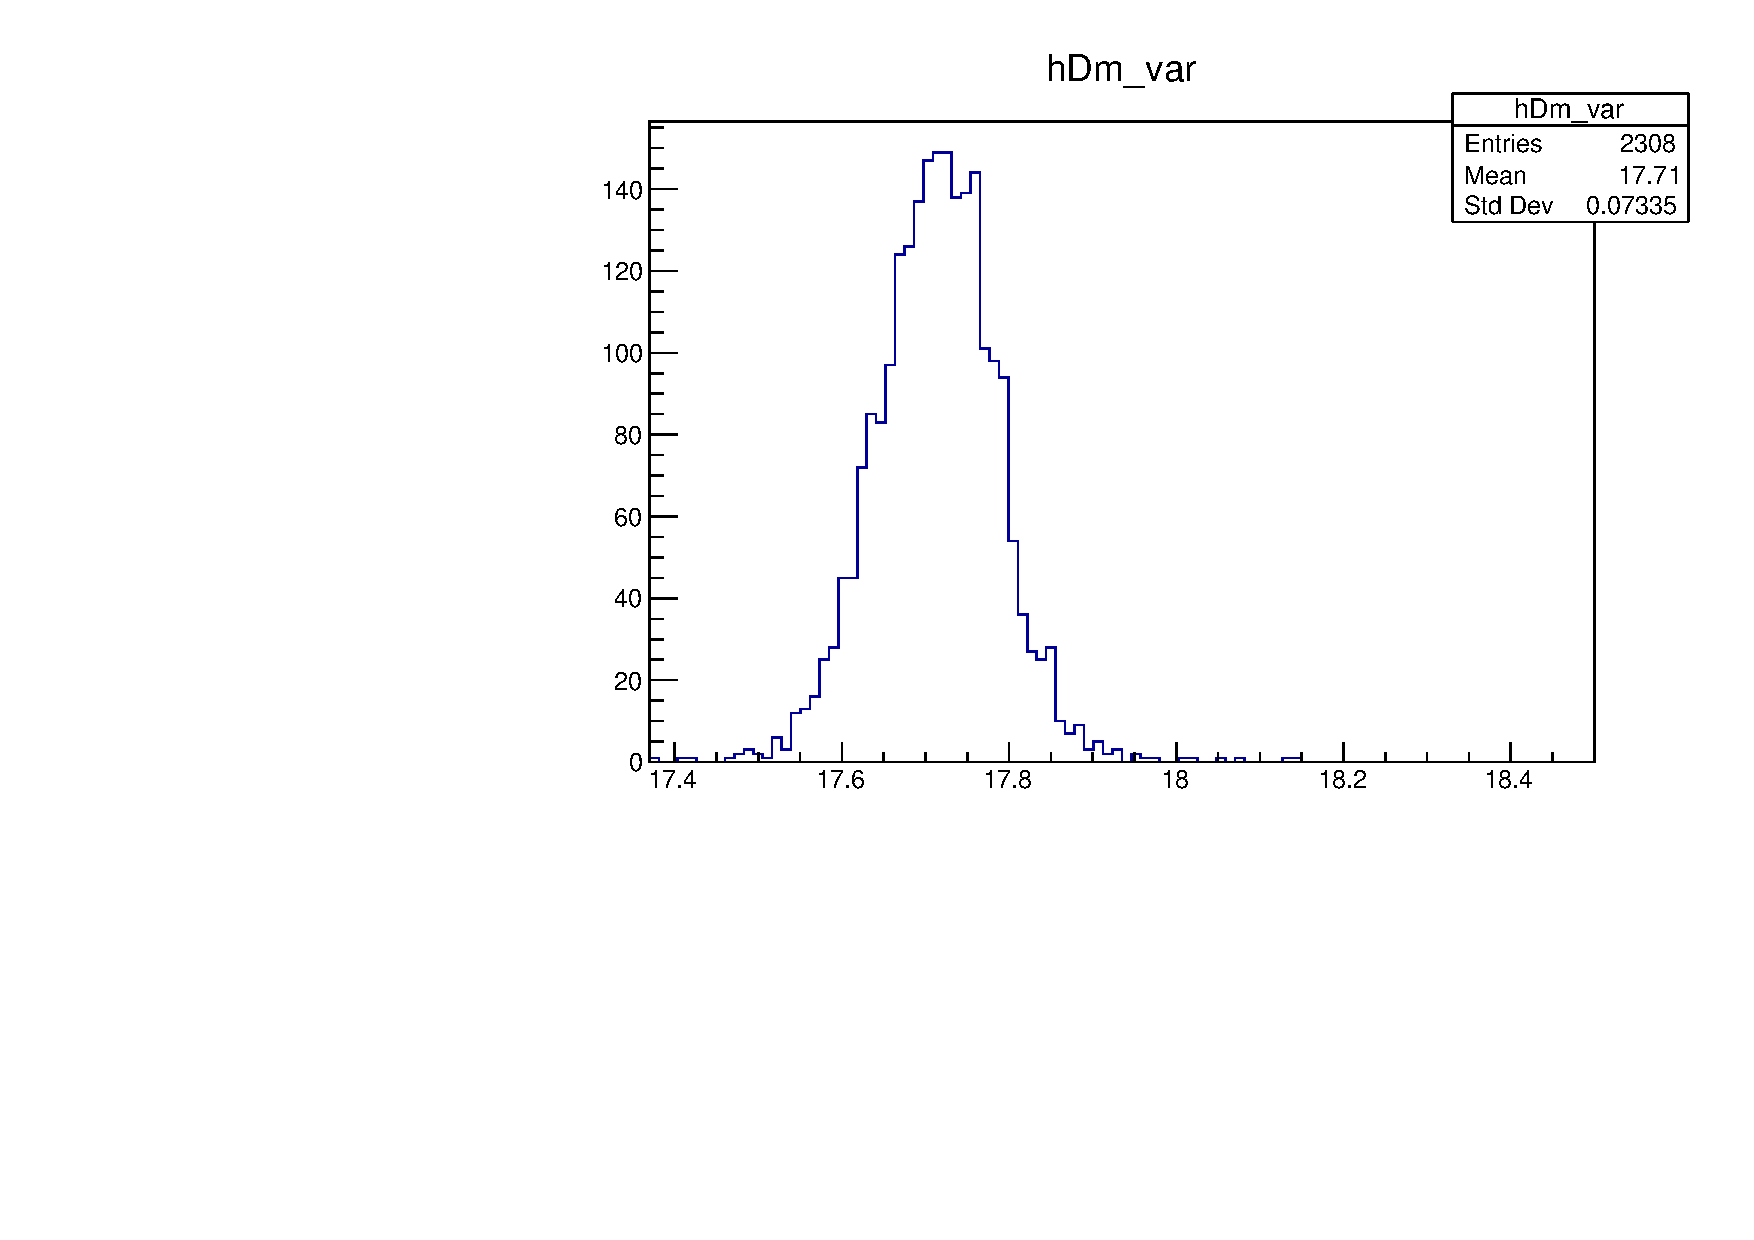
\includegraphics[width=0.3\textwidth]{figs/DataVars/Dm_var.pdf}
	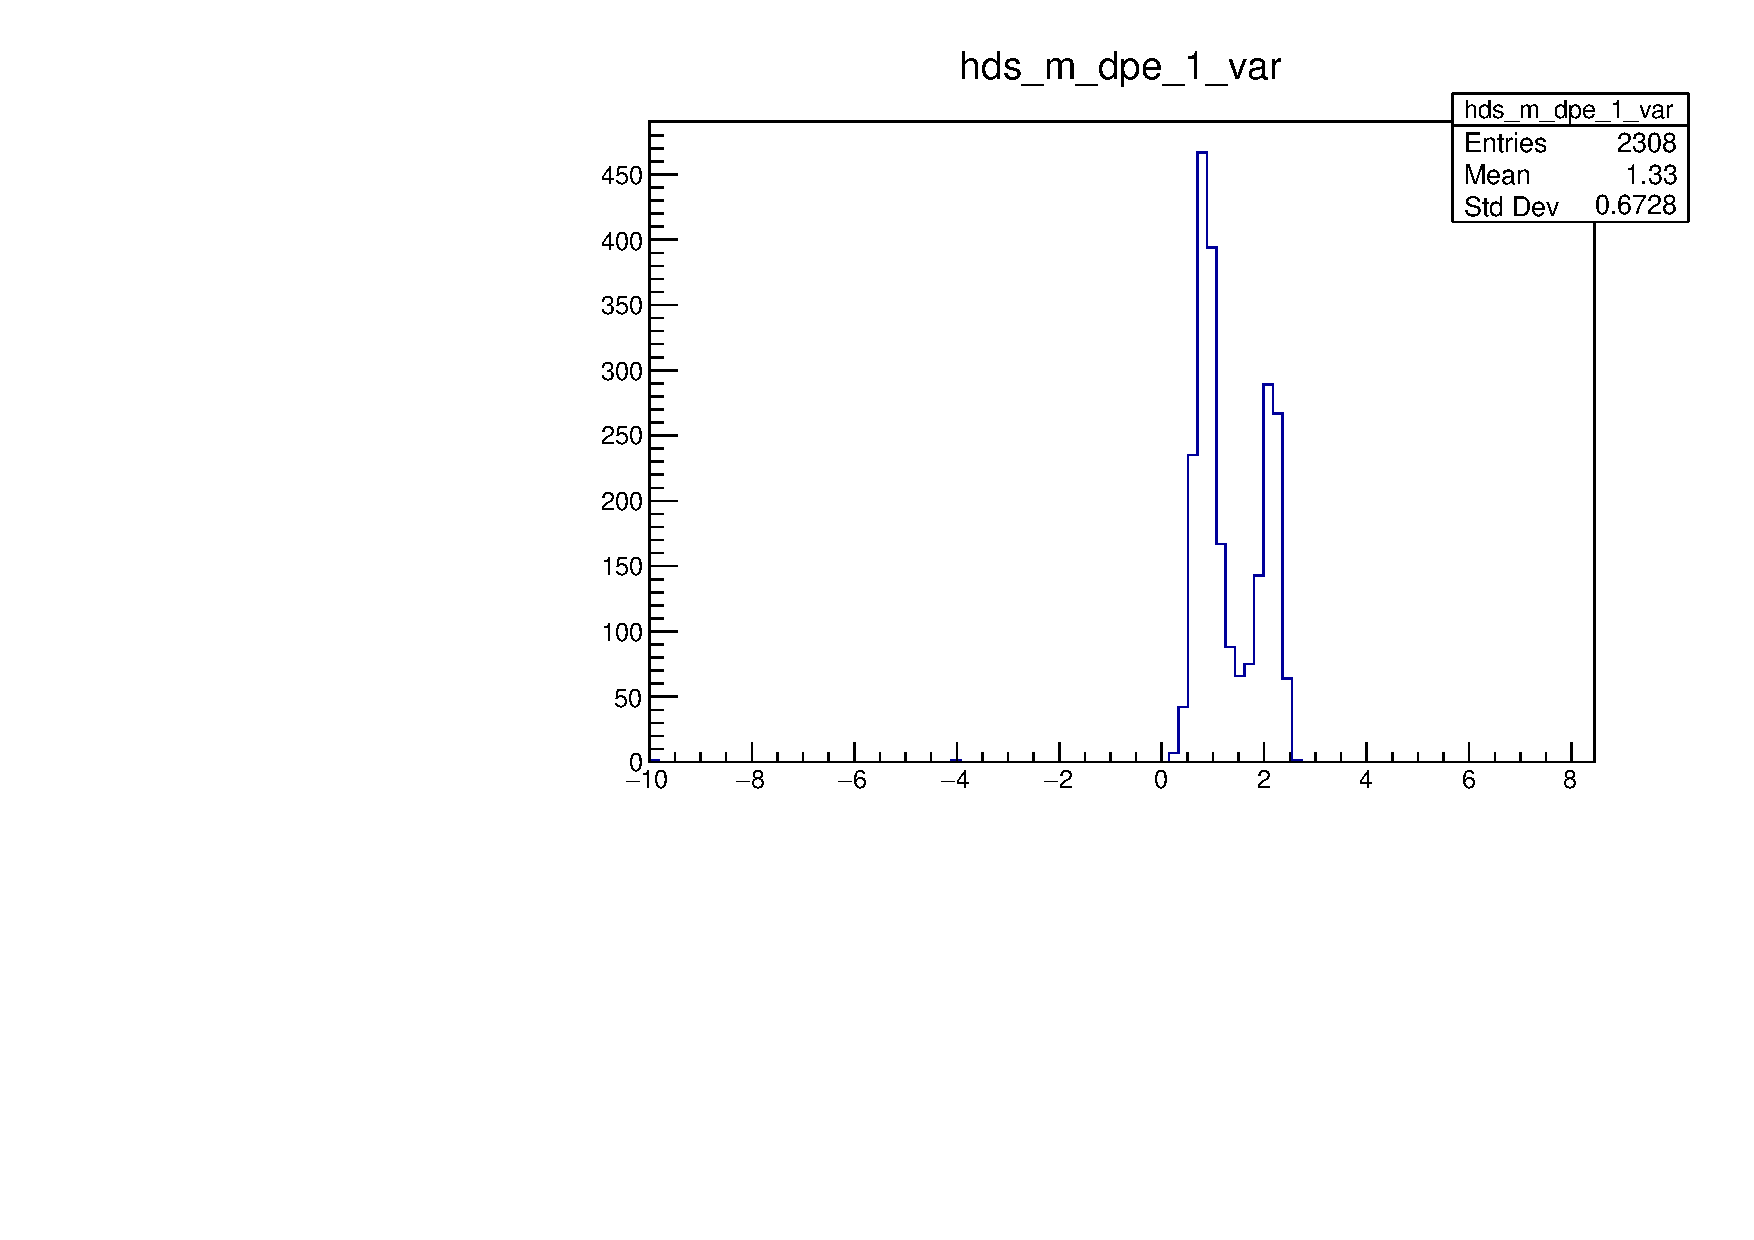
\includegraphics[width=0.3\textwidth]{figs/DataVars/ds_m_dpe_1_var.pdf}
	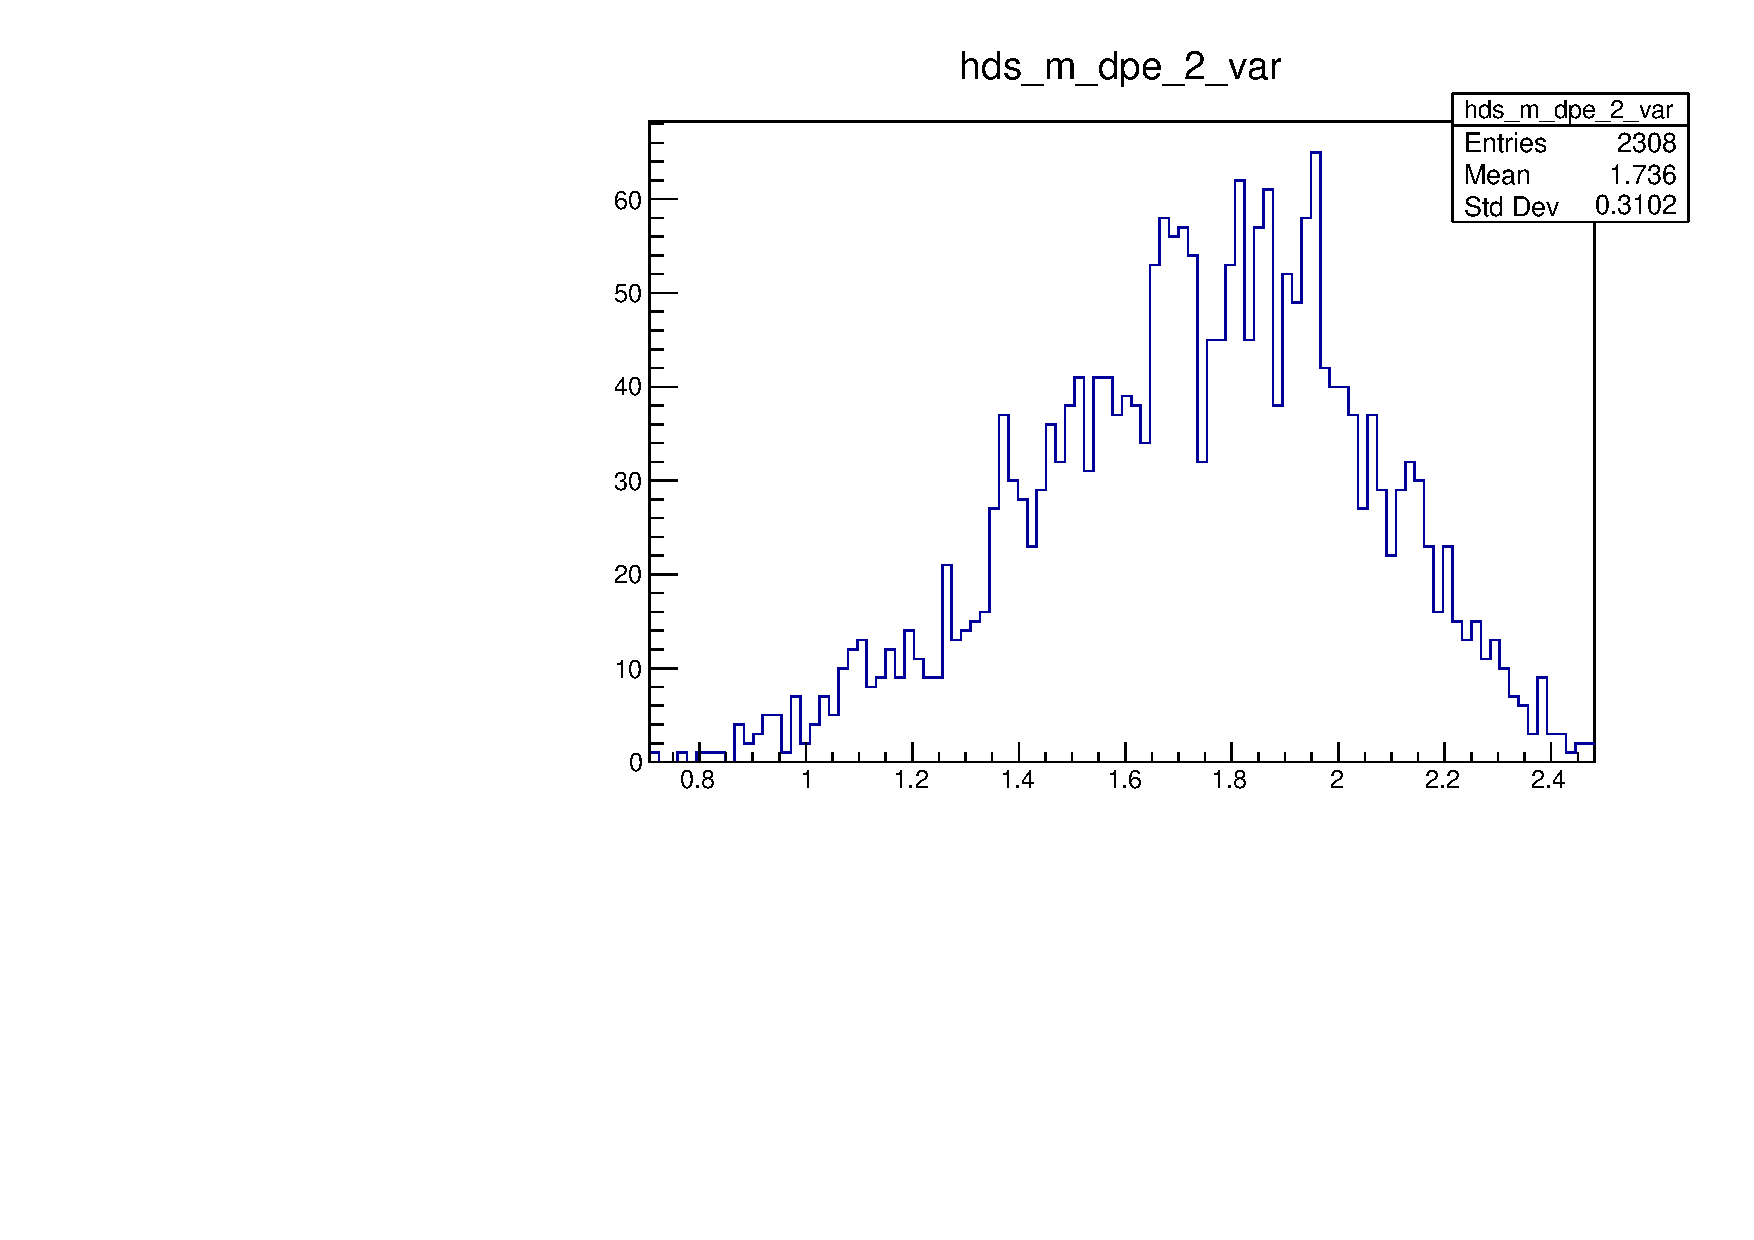
\includegraphics[width=0.3\textwidth]{figs/DataVars/ds_m_dpe_2_var.pdf}
	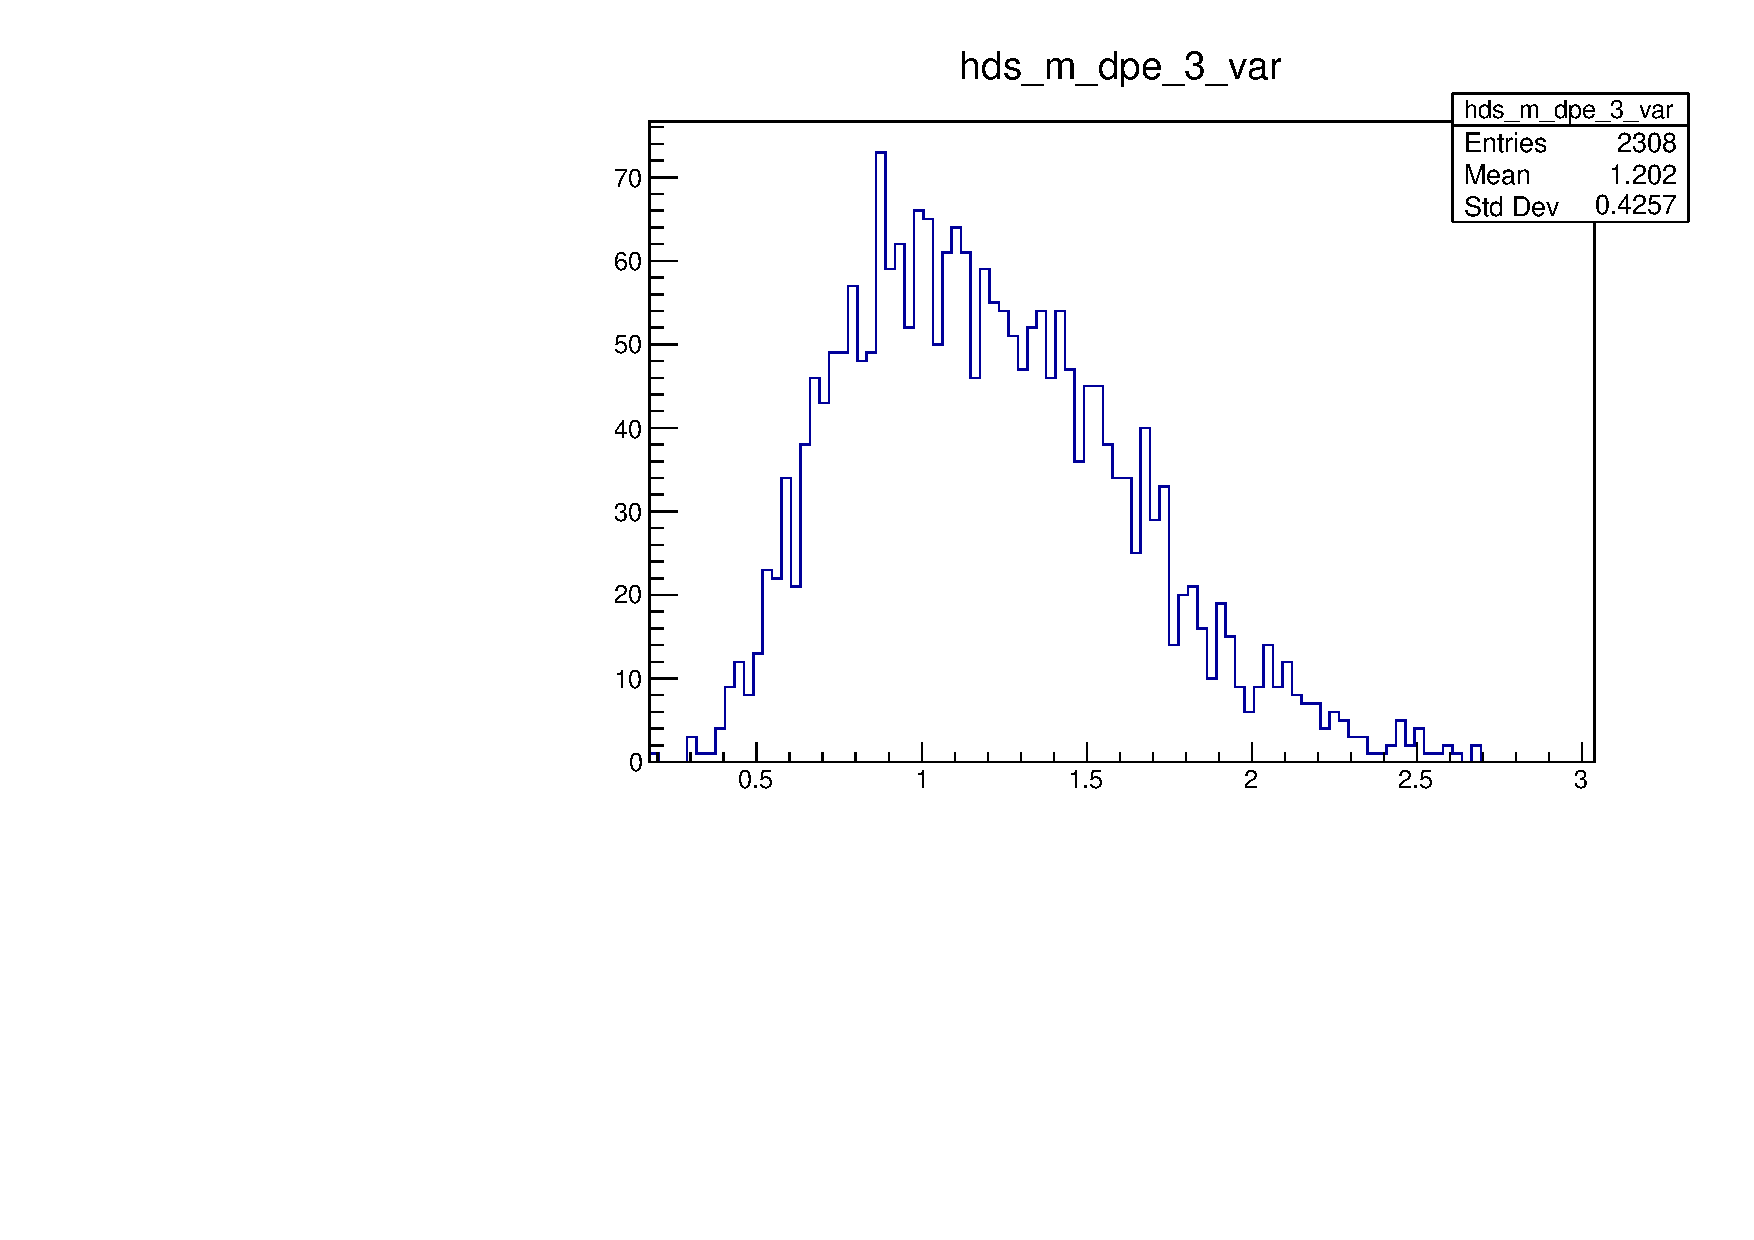
\includegraphics[width=0.3\textwidth]{figs/DataVars/ds_m_dpe_3_var.pdf}
	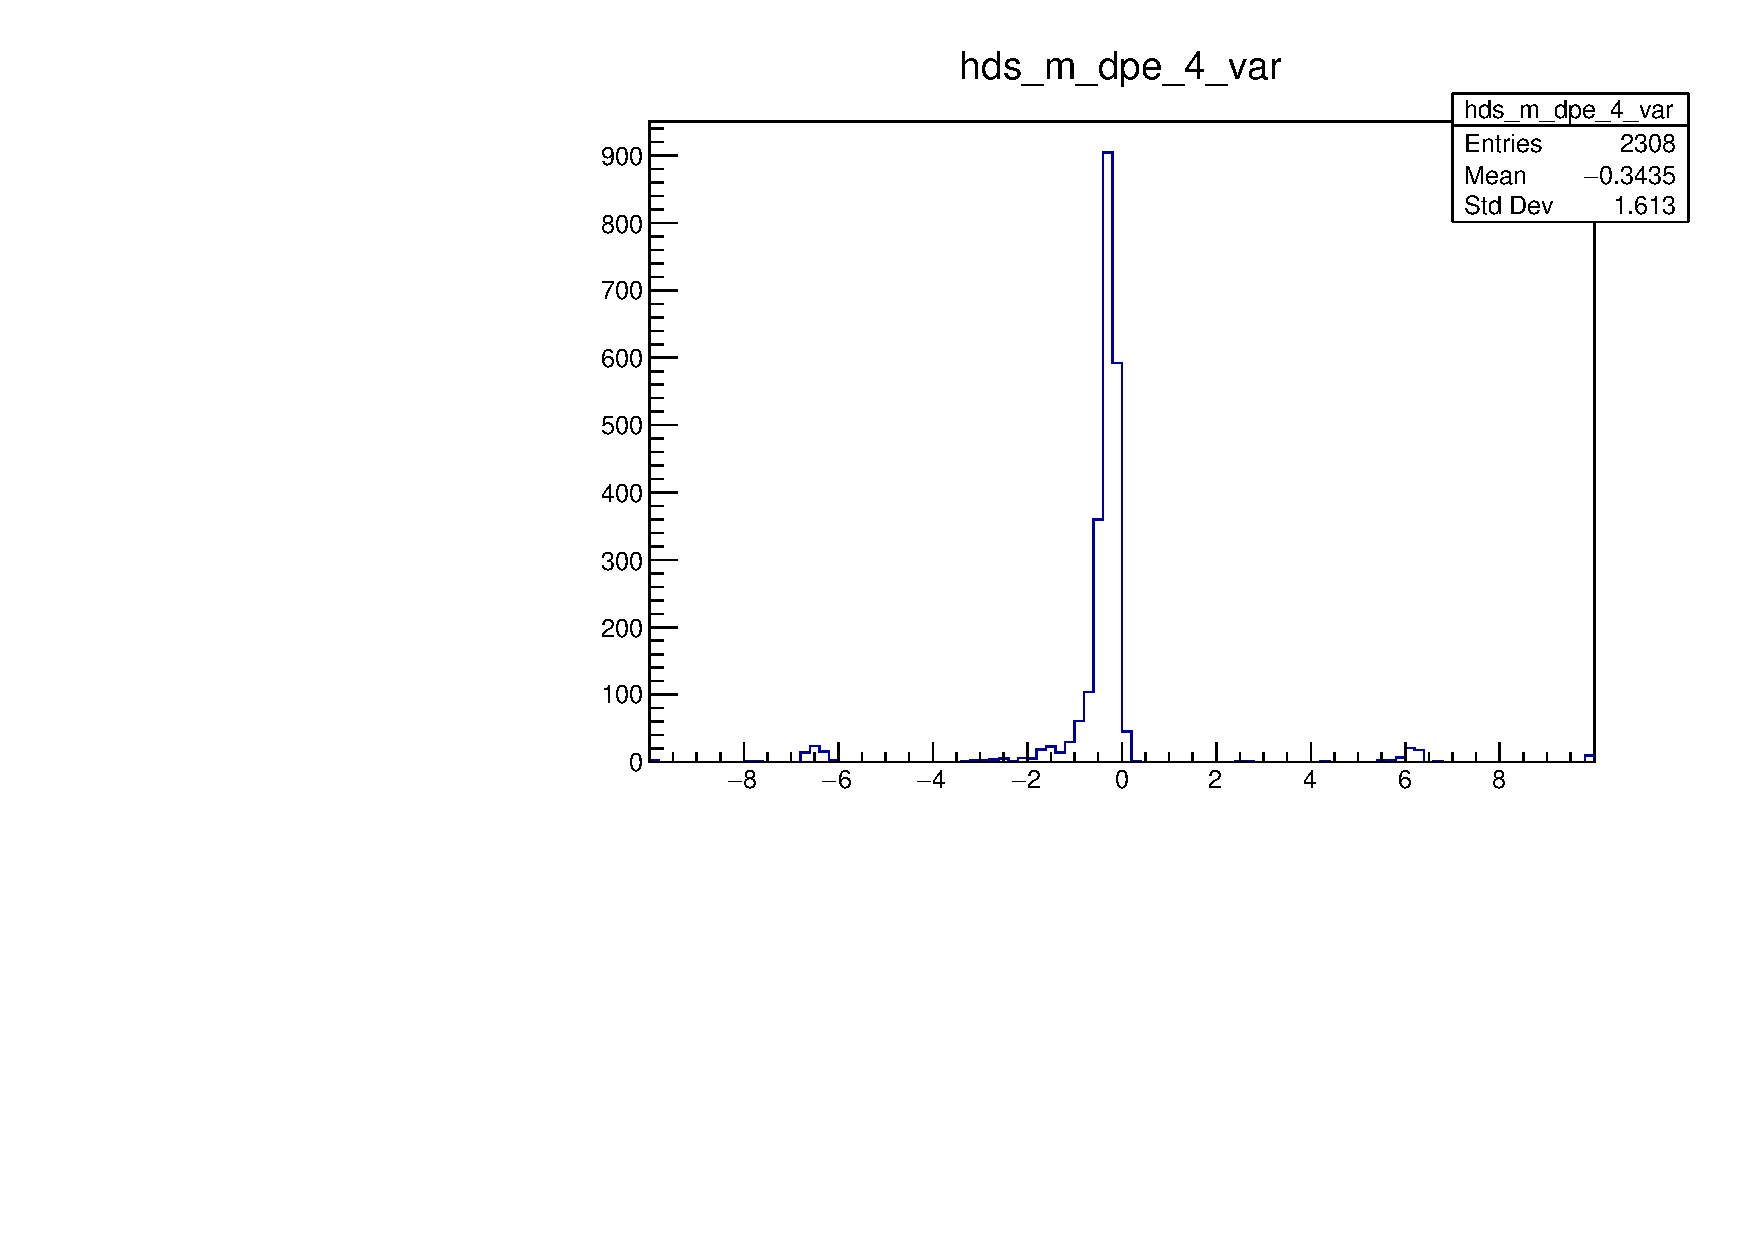
\includegraphics[width=0.3\textwidth]{figs/DataVars/ds_m_dpe_4_var.pdf}
	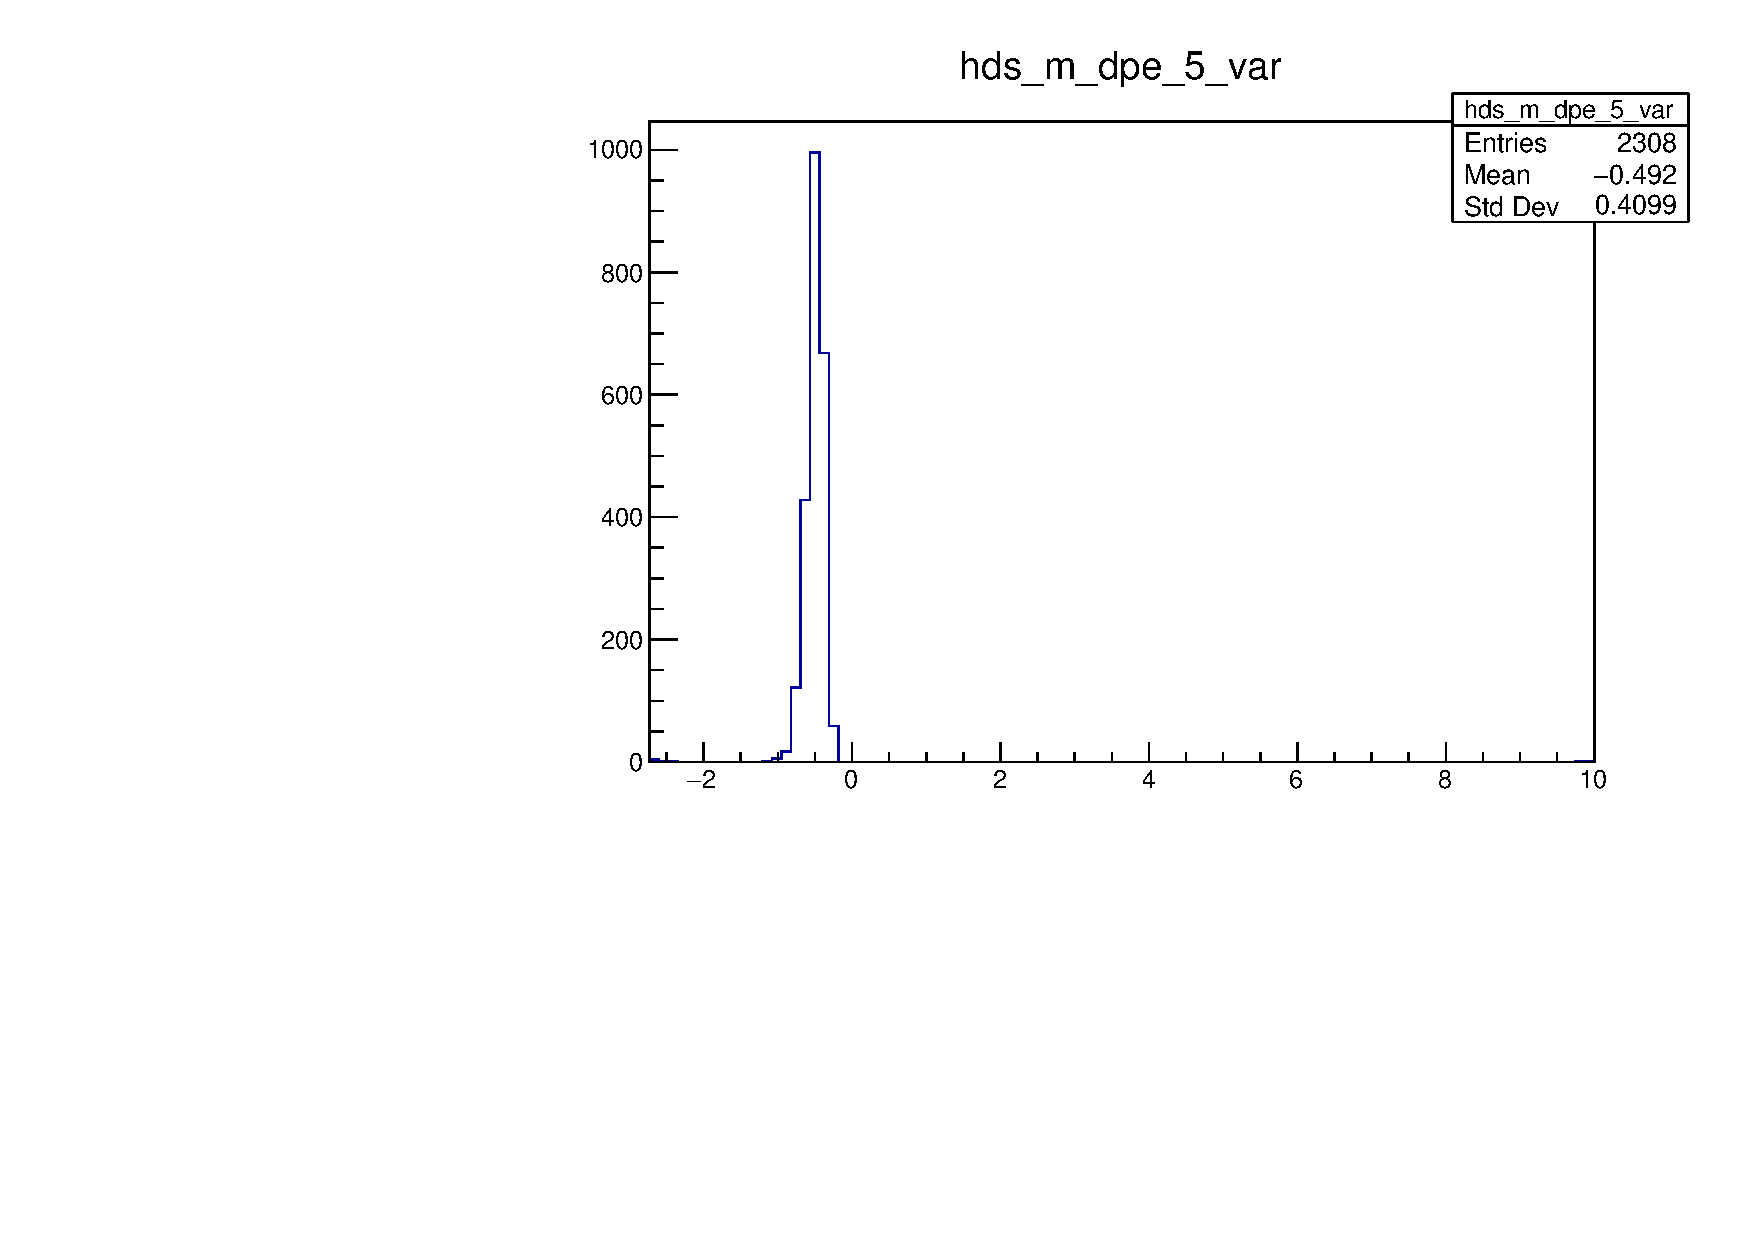
\includegraphics[width=0.3\textwidth]{figs/DataVars/ds_m_dpe_5_var.pdf}
	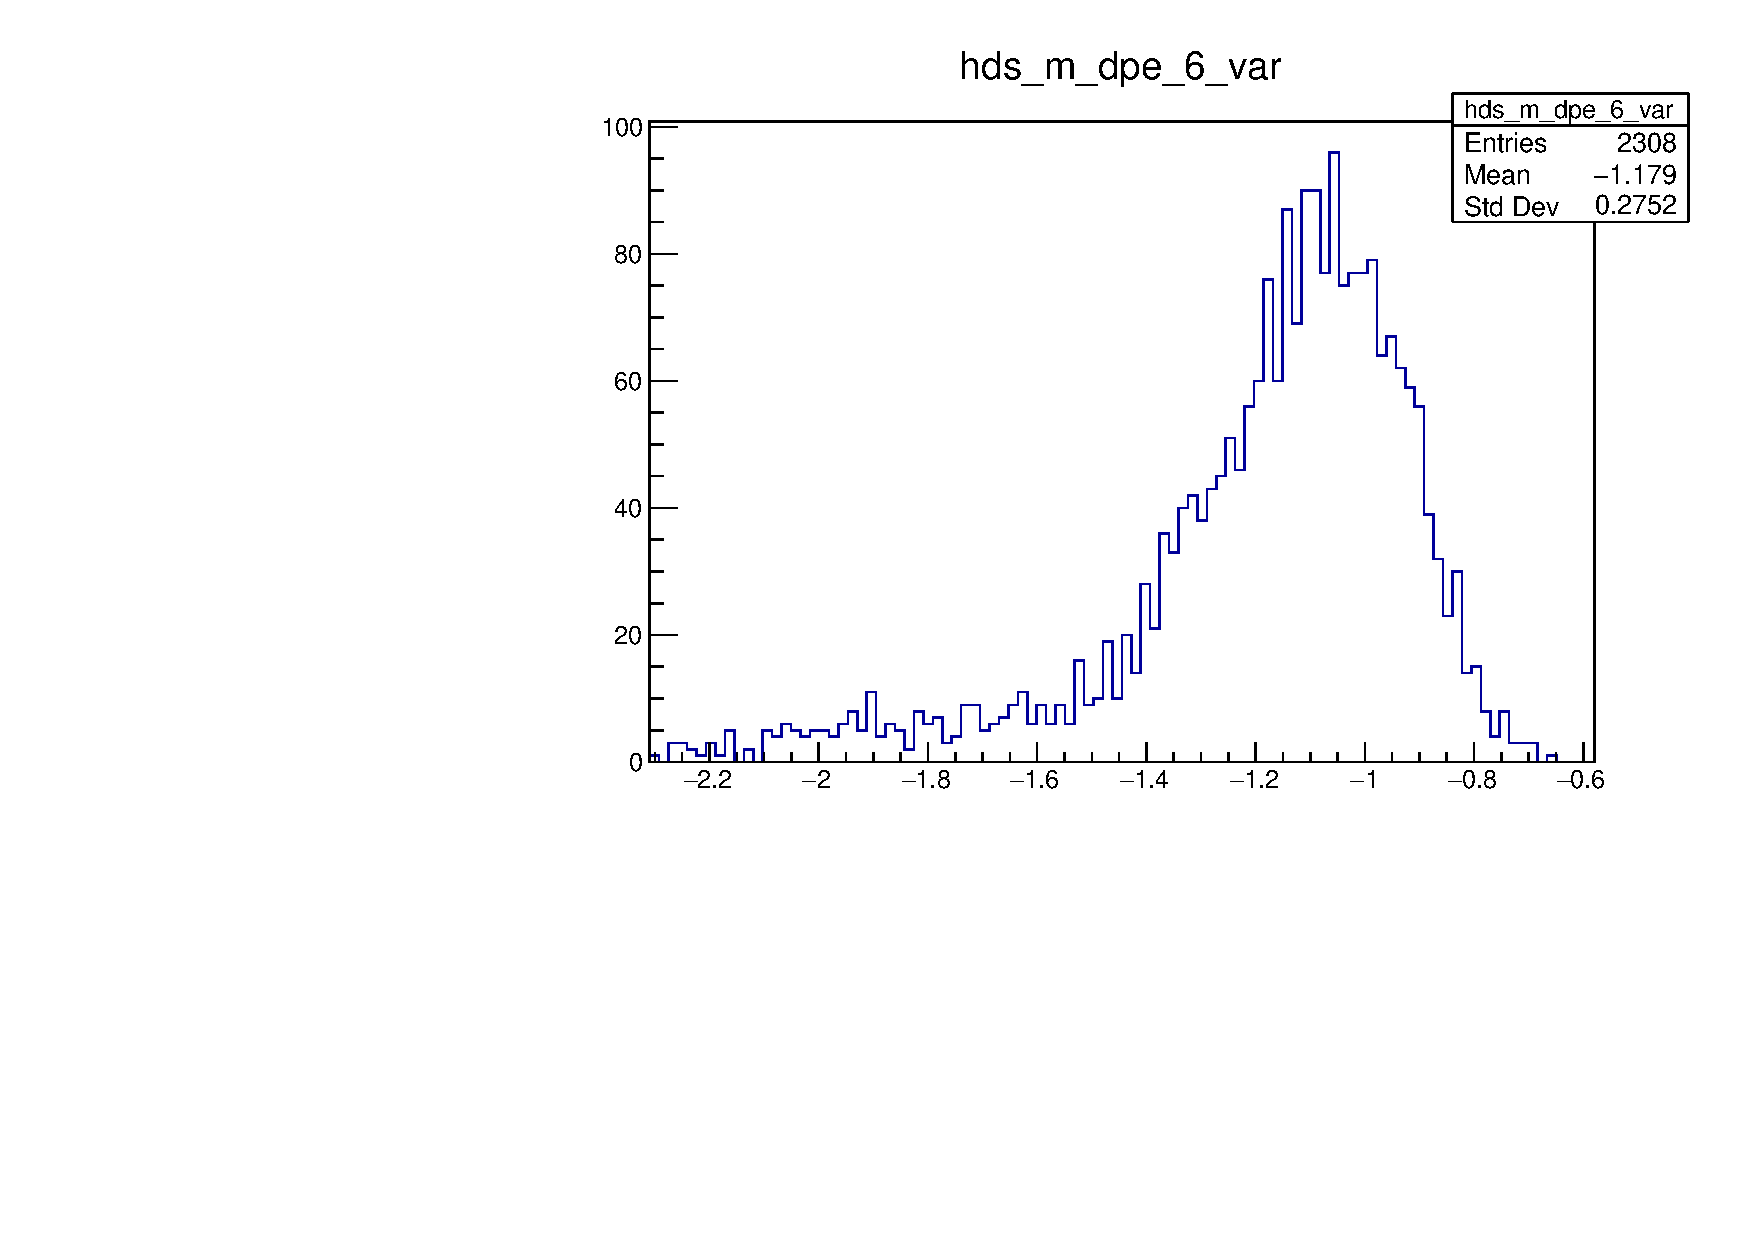
\includegraphics[width=0.3\textwidth]{figs/DataVars/ds_m_dpe_6_var.pdf}
	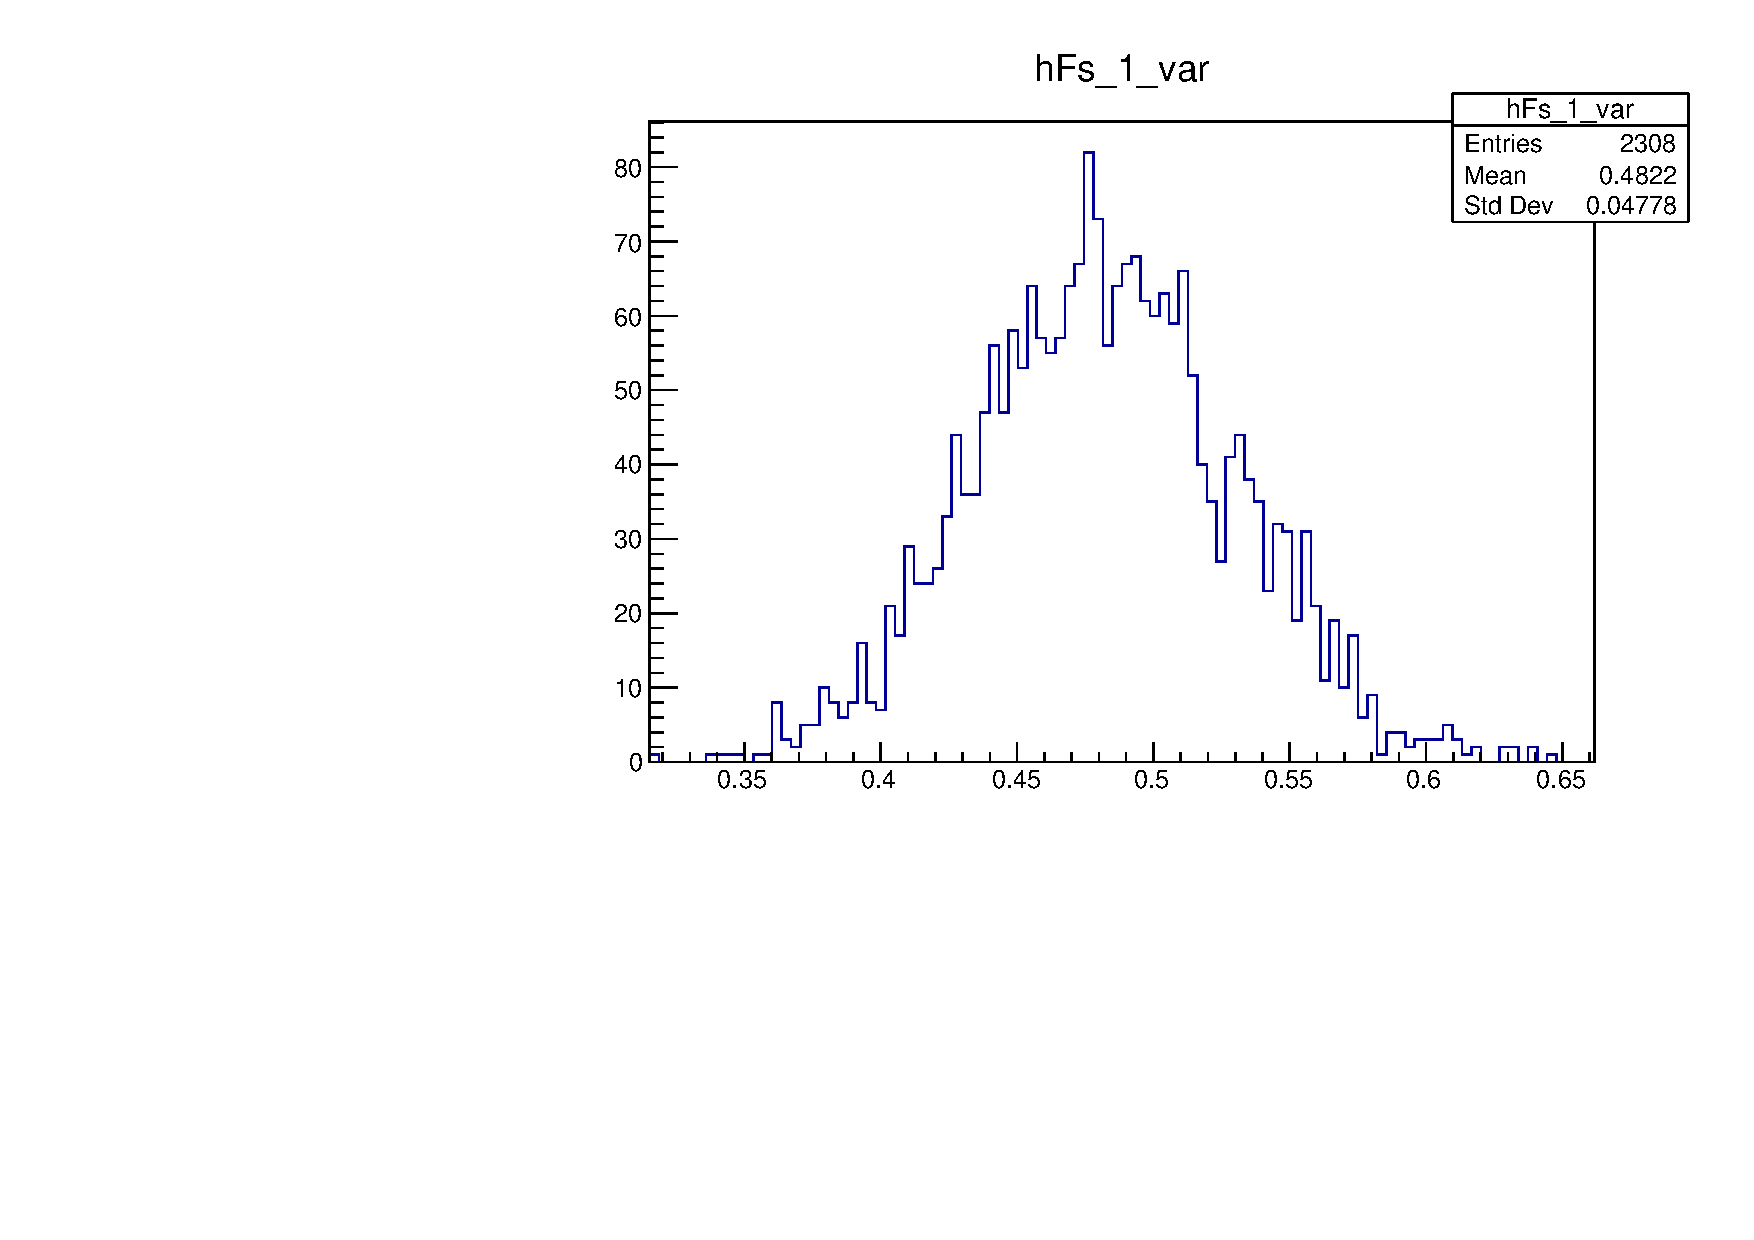
\includegraphics[width=0.3\textwidth]{figs/DataVars/Fs_1_var.pdf}
	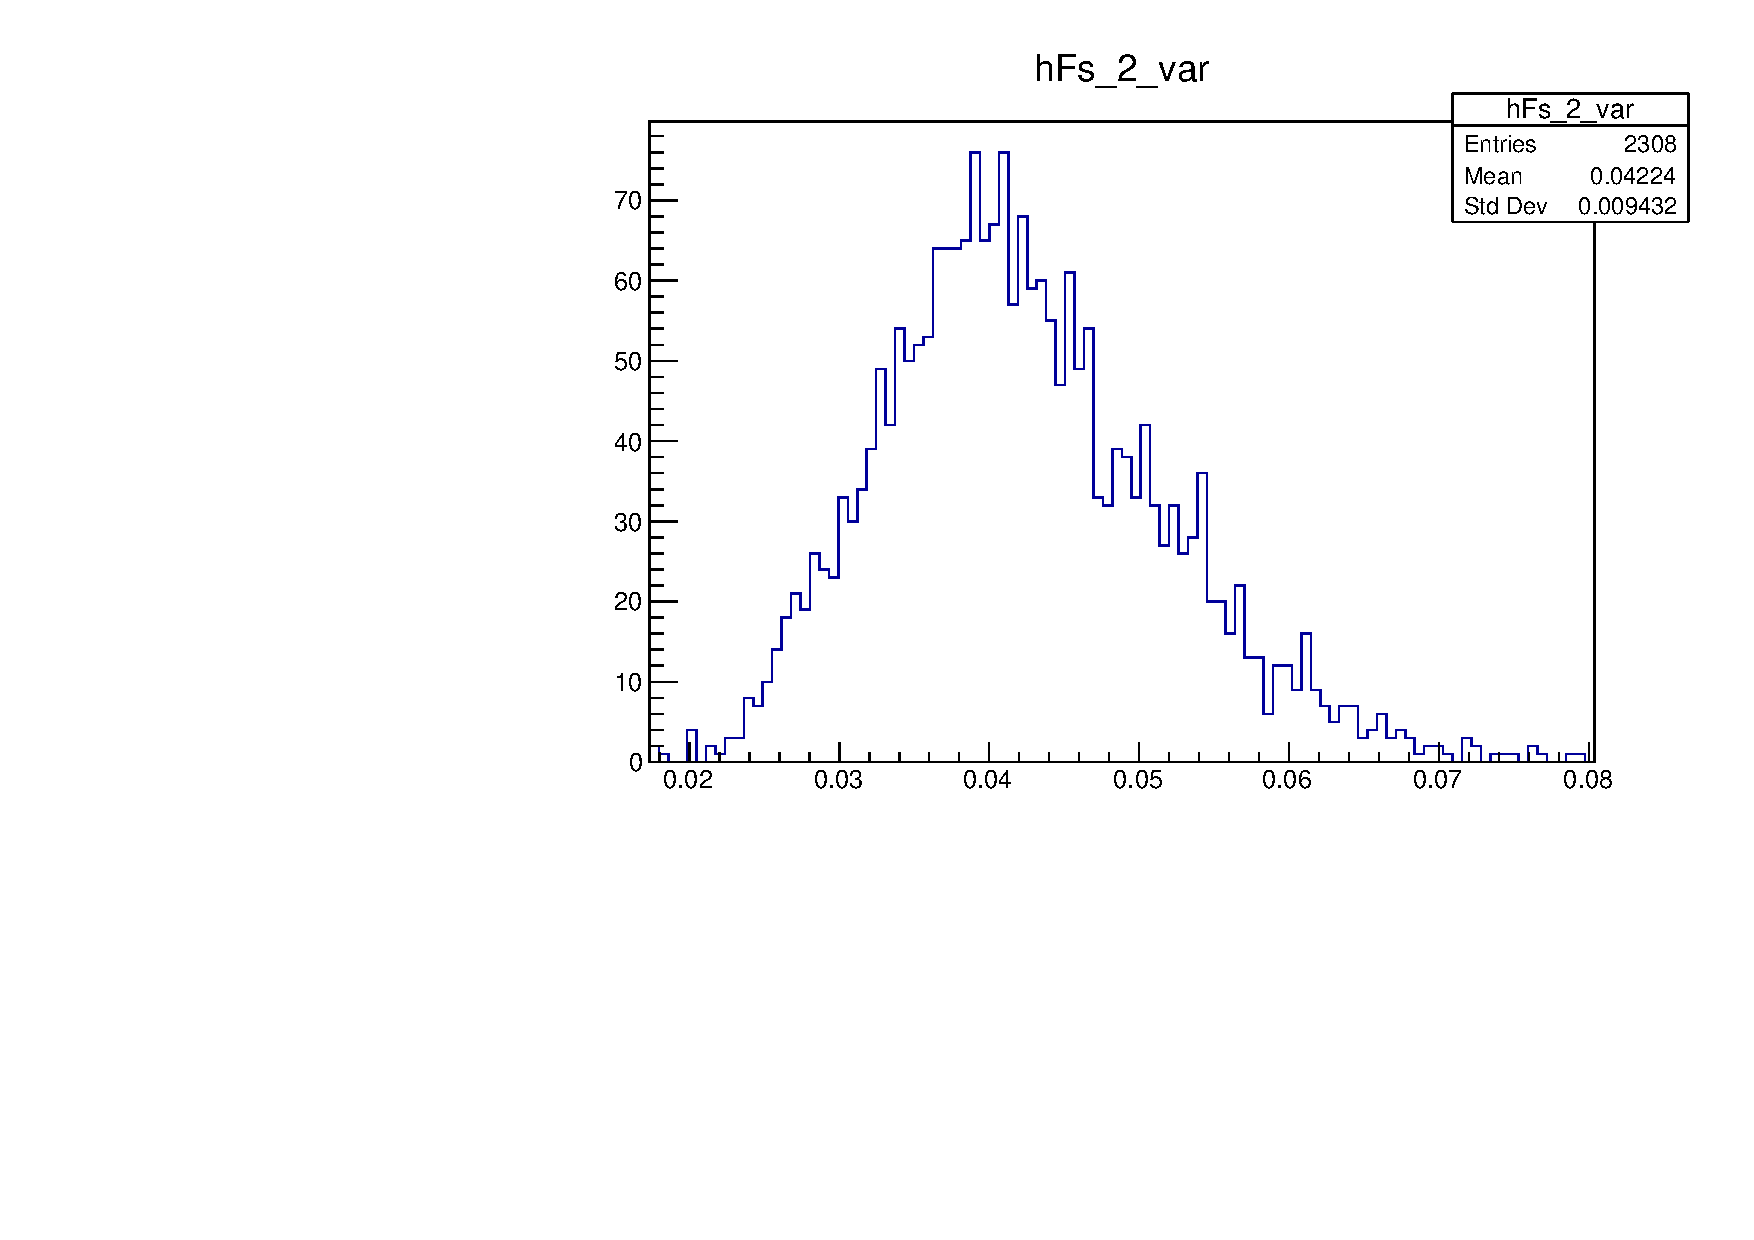
\includegraphics[width=0.3\textwidth]{figs/DataVars/Fs_2_var.pdf}
	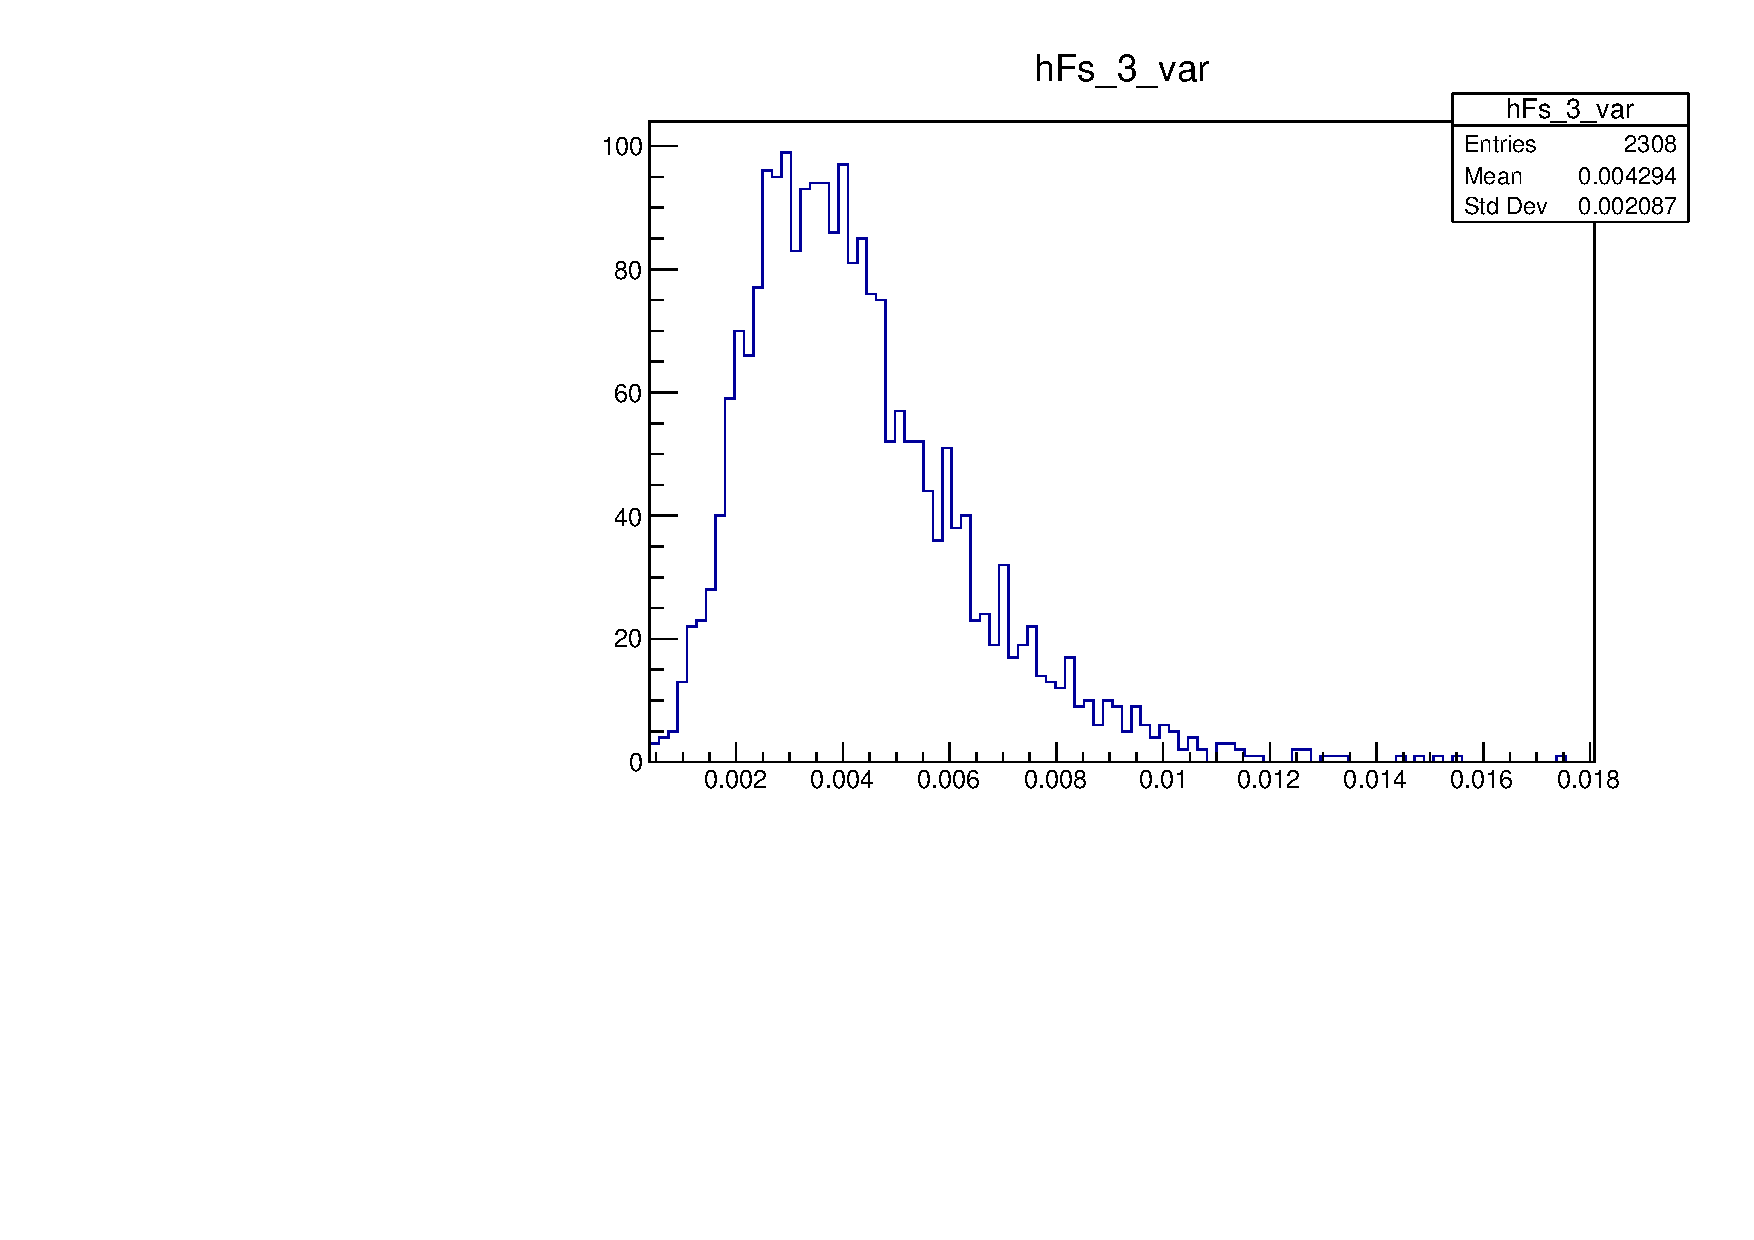
\includegraphics[width=0.3\textwidth]{figs/DataVars/Fs_3_var.pdf}
	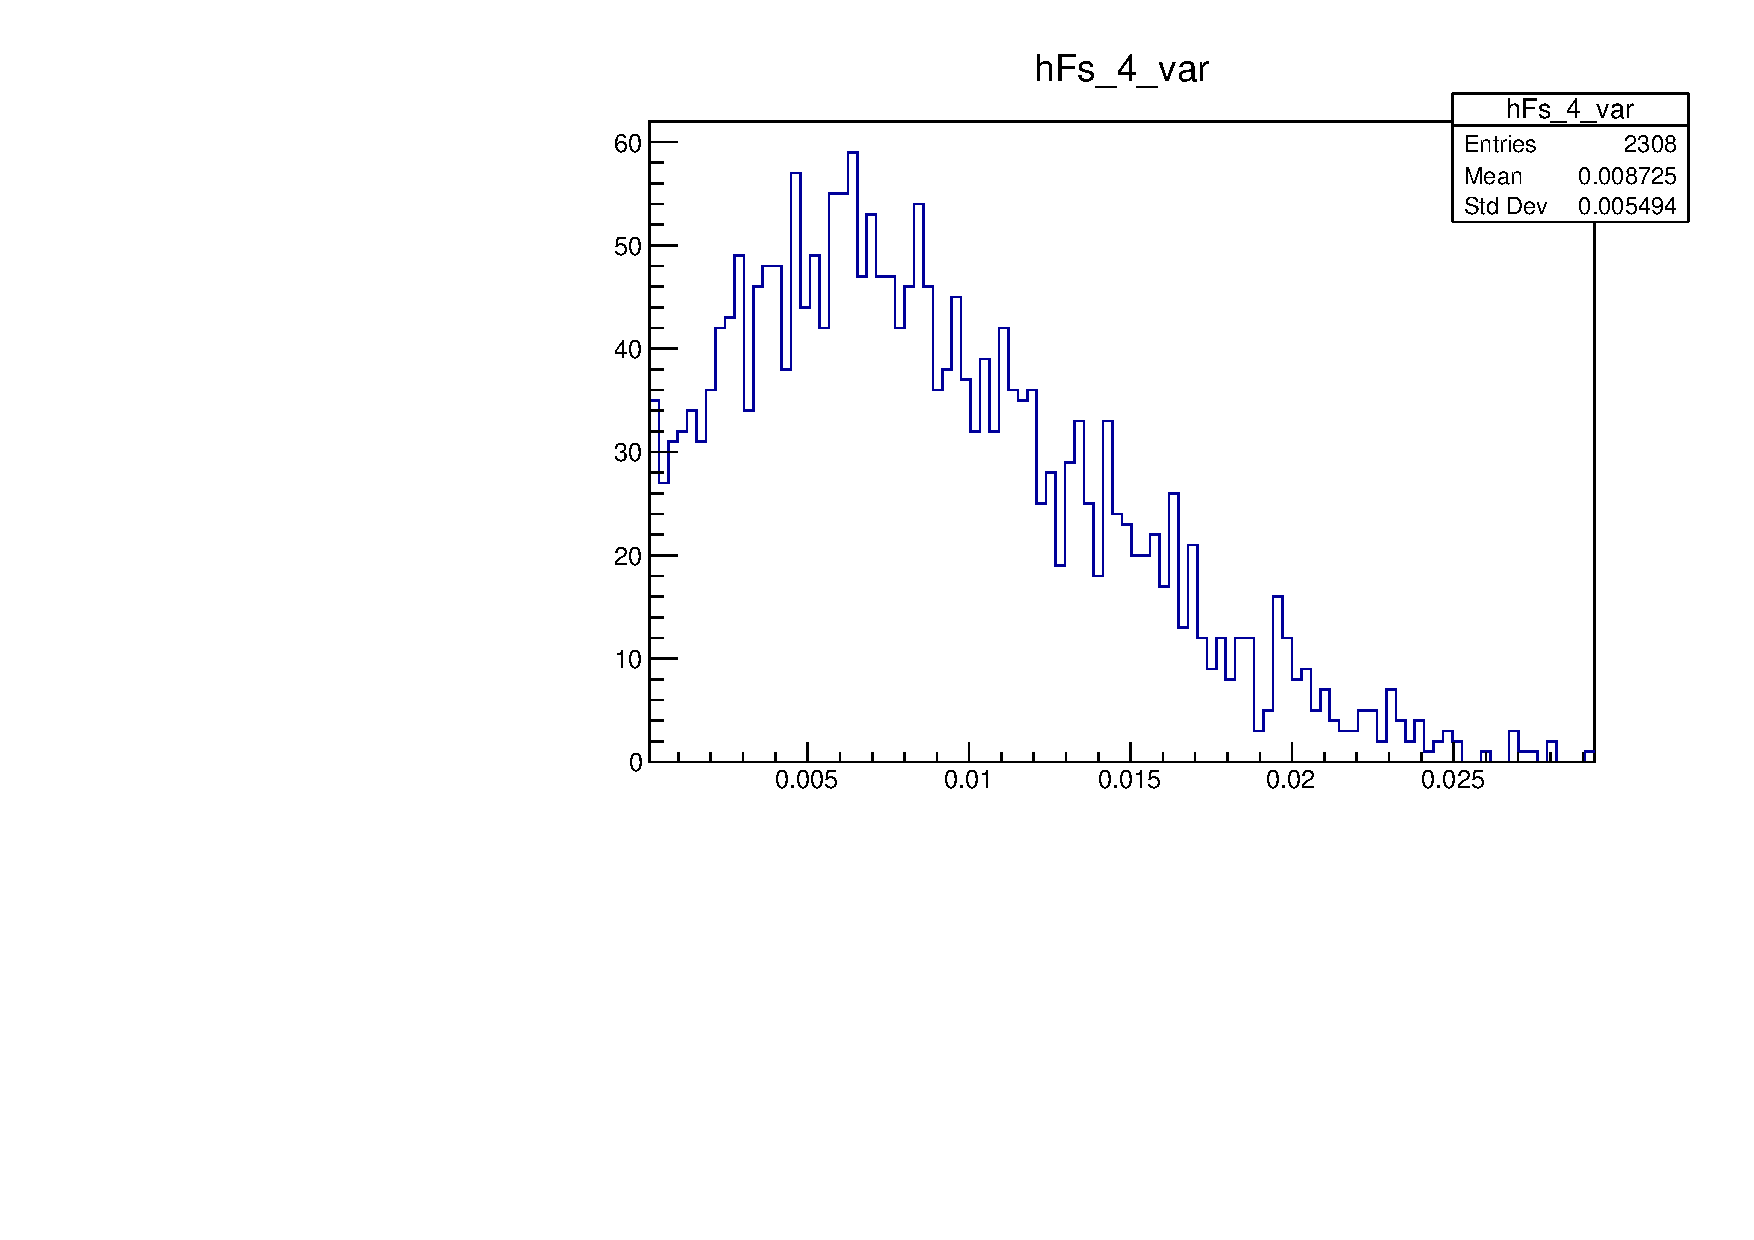
\includegraphics[width=0.3\textwidth]{figs/DataVars/Fs_4_var.pdf}
	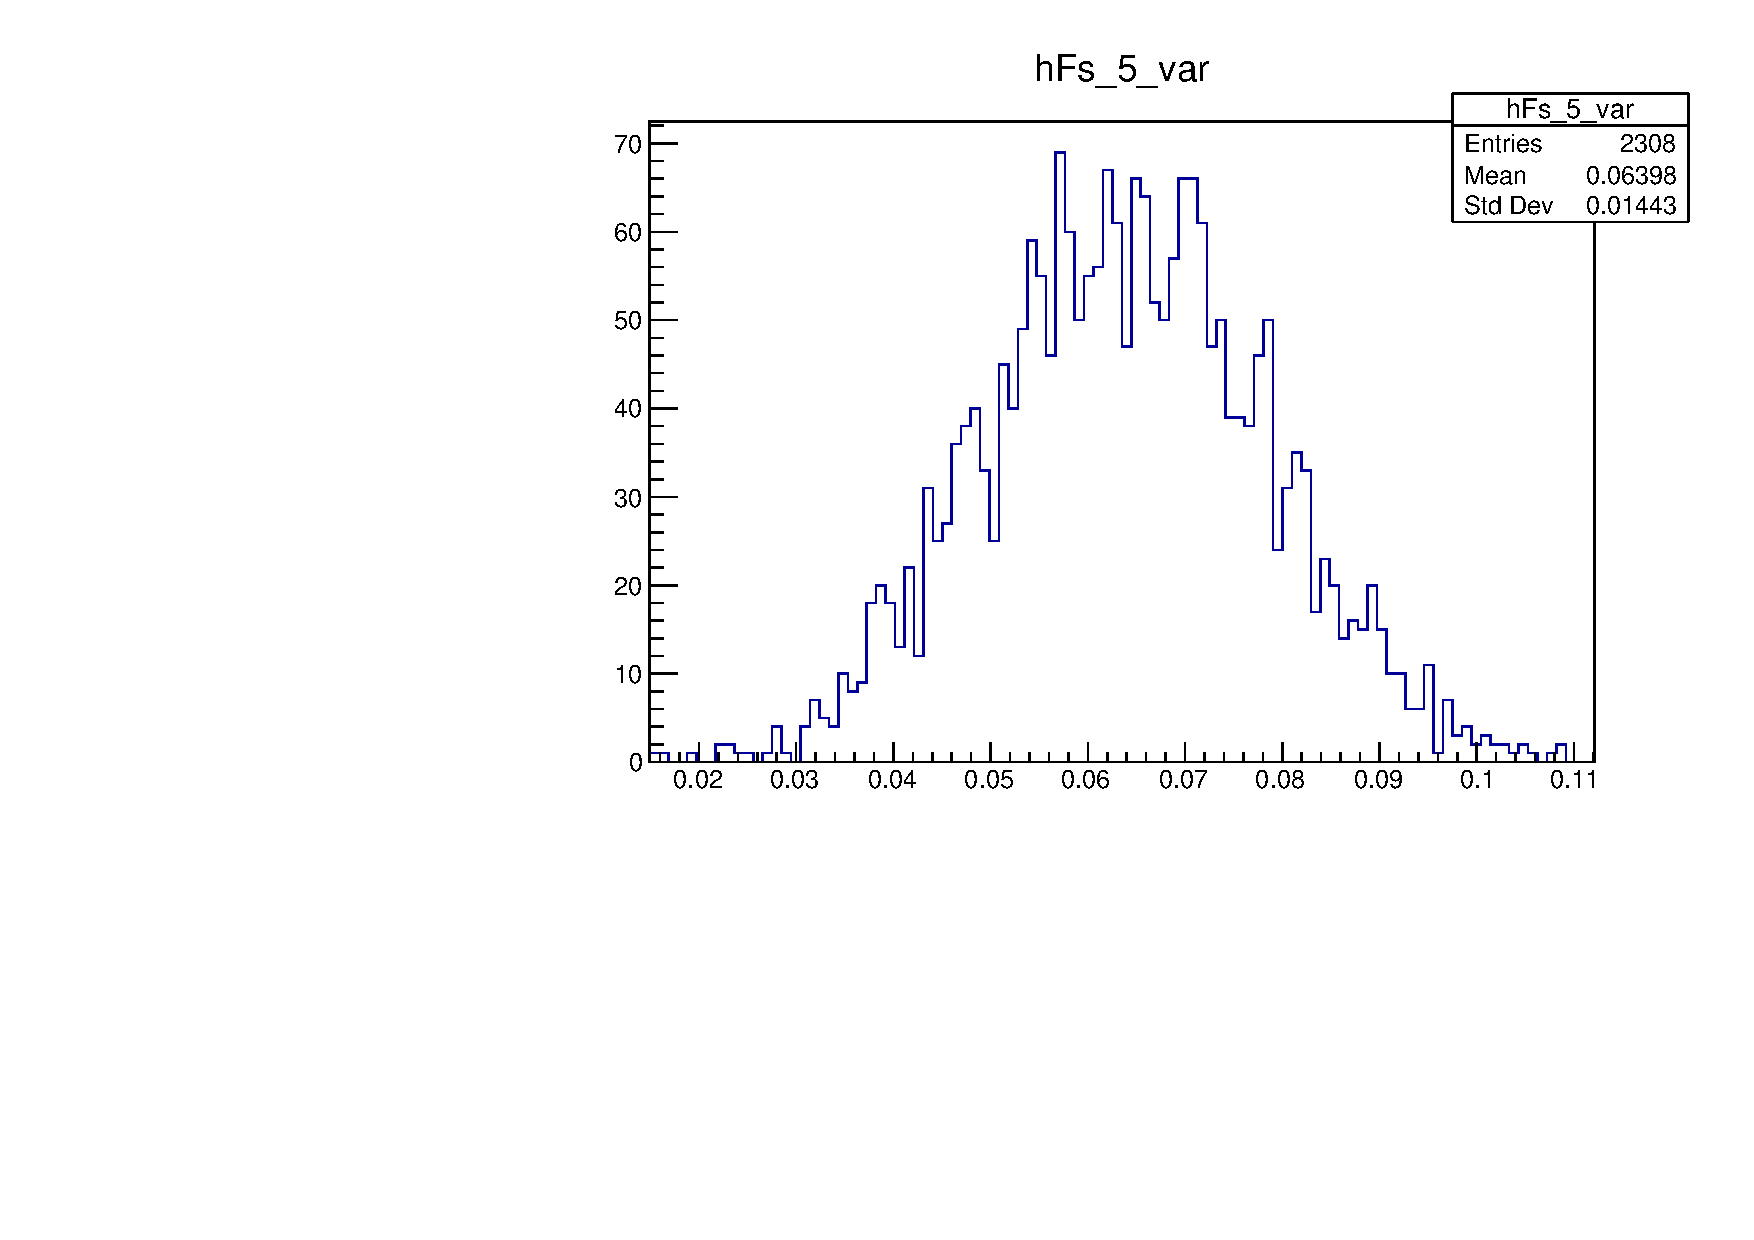
\includegraphics[width=0.3\textwidth]{figs/DataVars/Fs_5_var.pdf}
	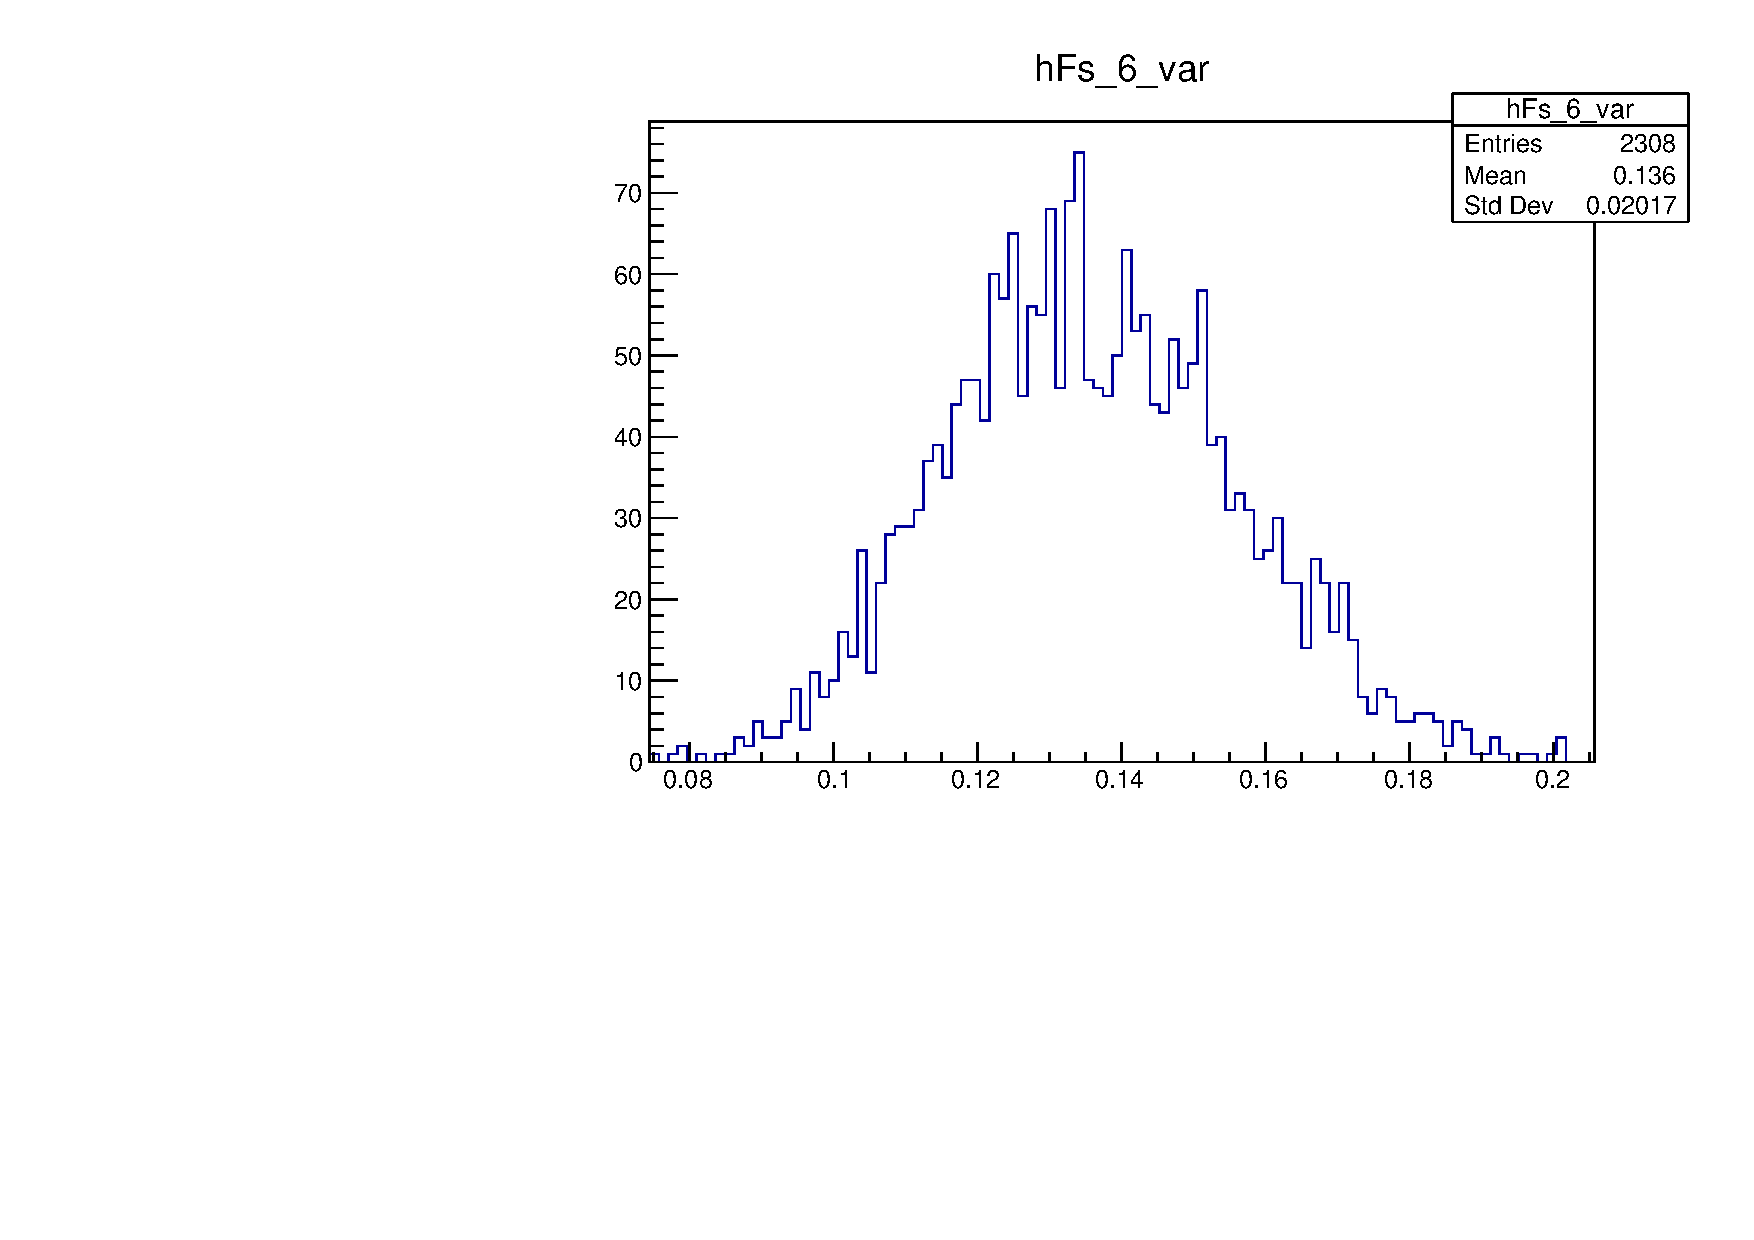
\includegraphics[width=0.3\textwidth]{figs/DataVars/Fs_6_var.pdf}
   \end{center}
   \caption{
	Distributions of the fit parameters using bootstrapping (data).
   }
   \label{fig:Vars_Data}
\end{figure}

\begin{figure}[tb]
   \begin{center}
	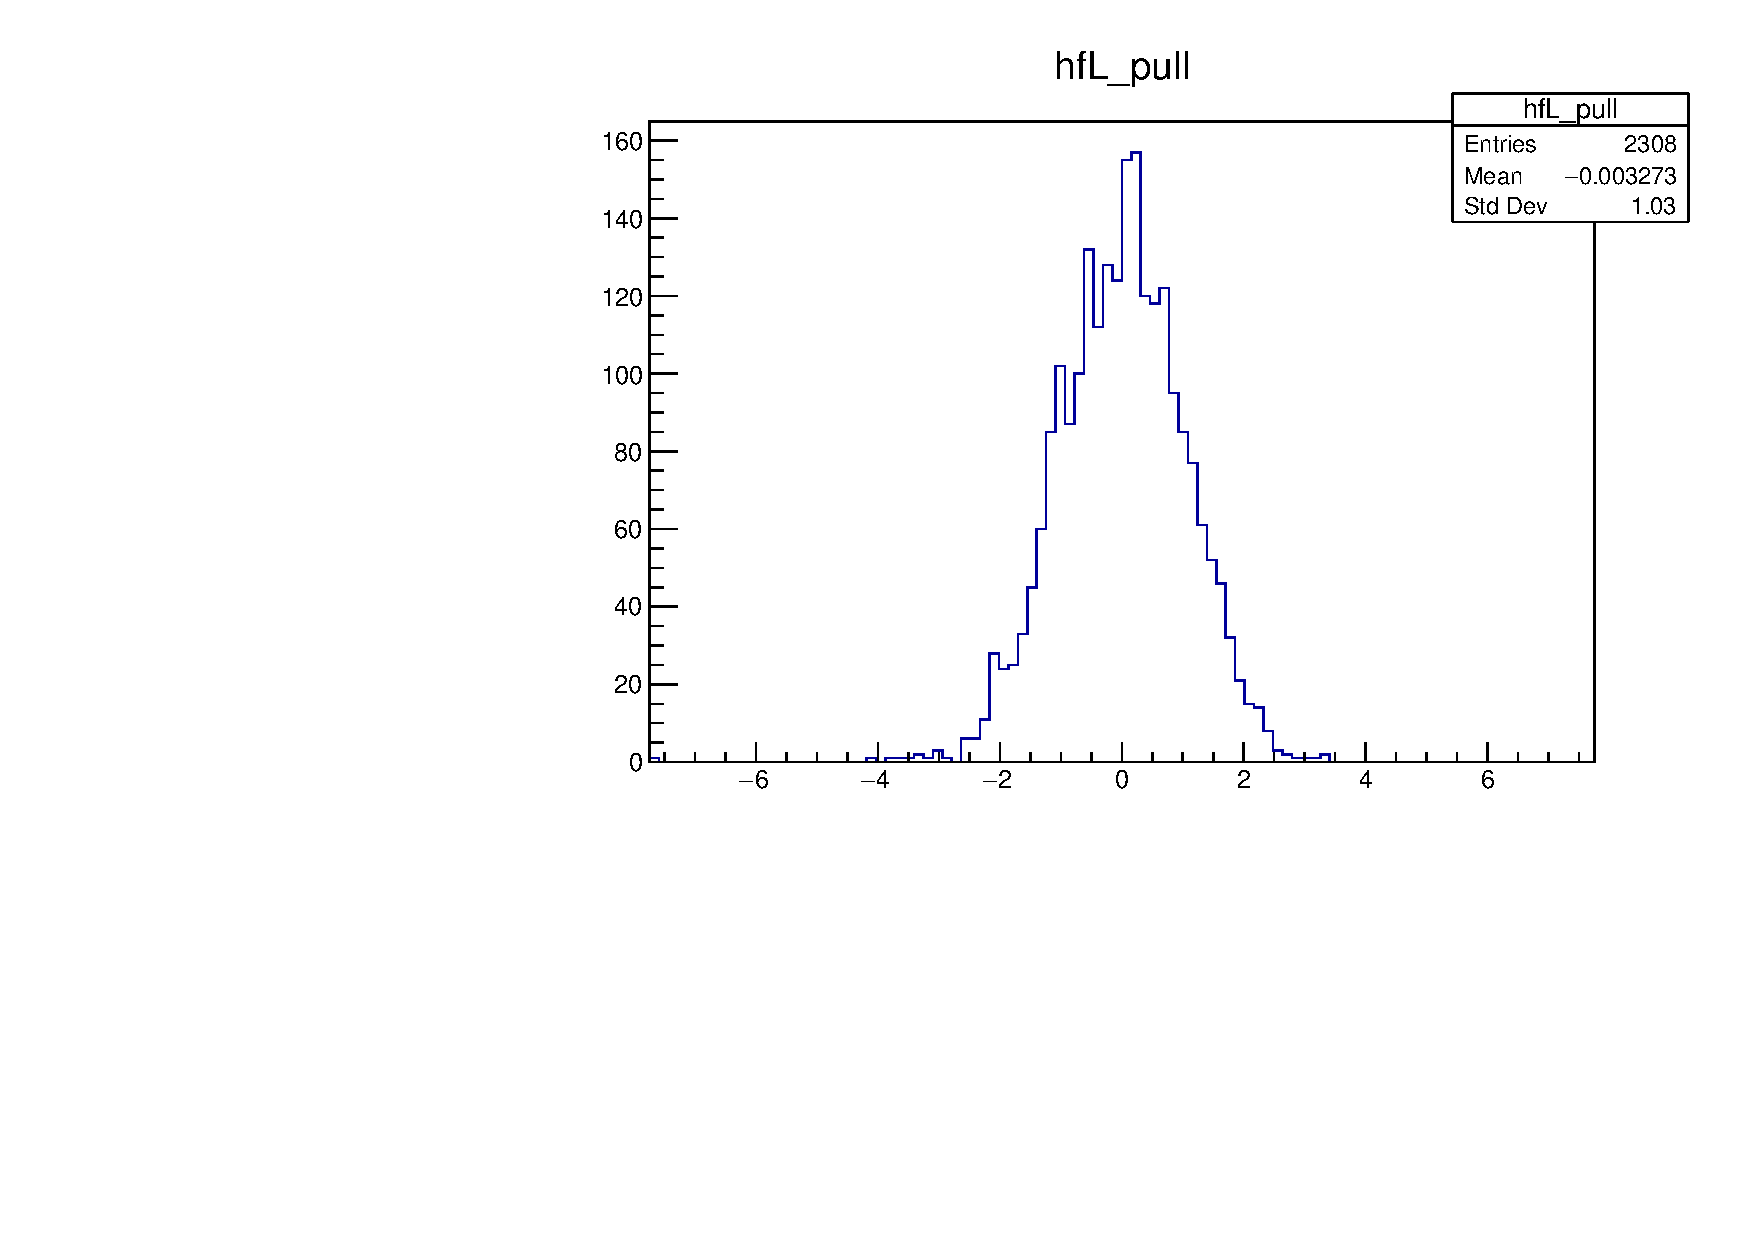
\includegraphics[width=0.3\textwidth]{figs/DataPulls/fL_pull.pdf}
	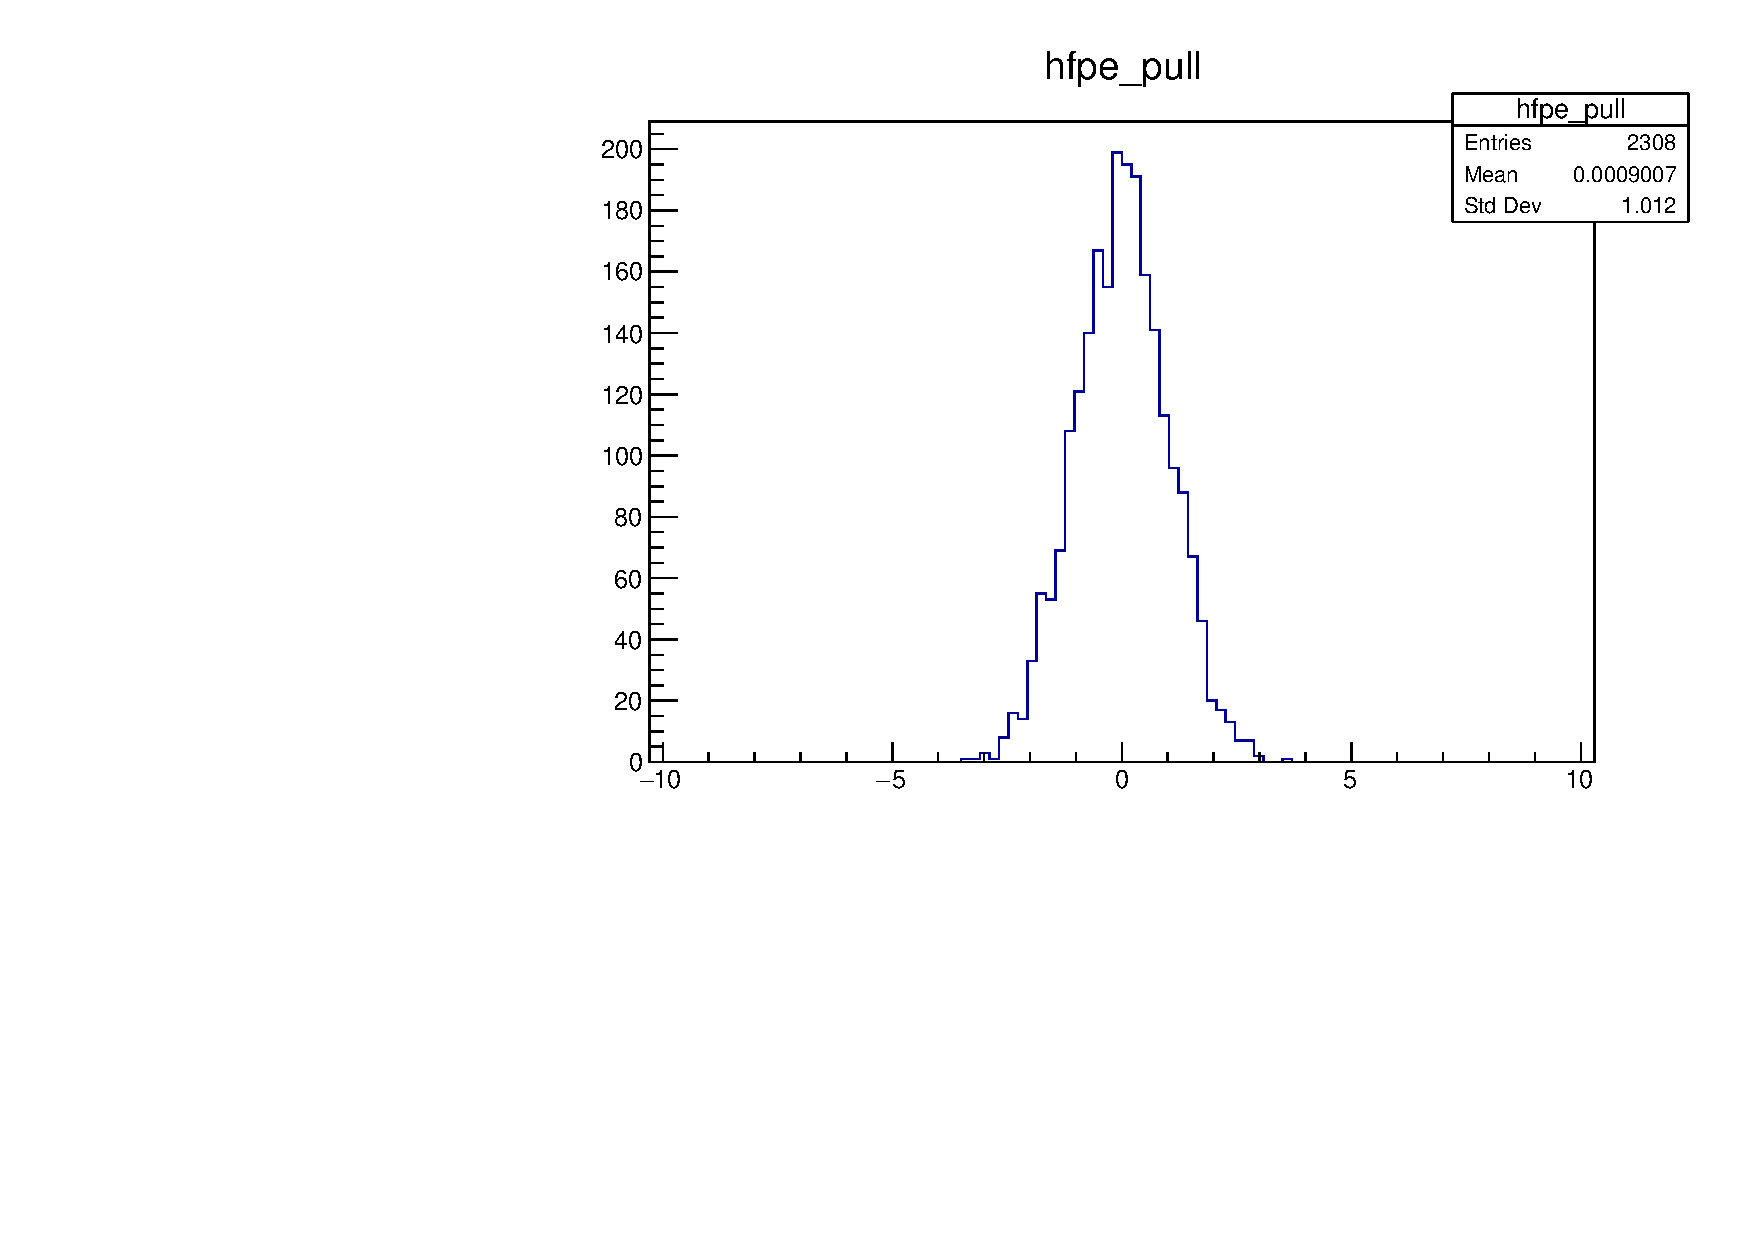
\includegraphics[width=0.3\textwidth]{figs/DataPulls/fpe_pull.pdf}
	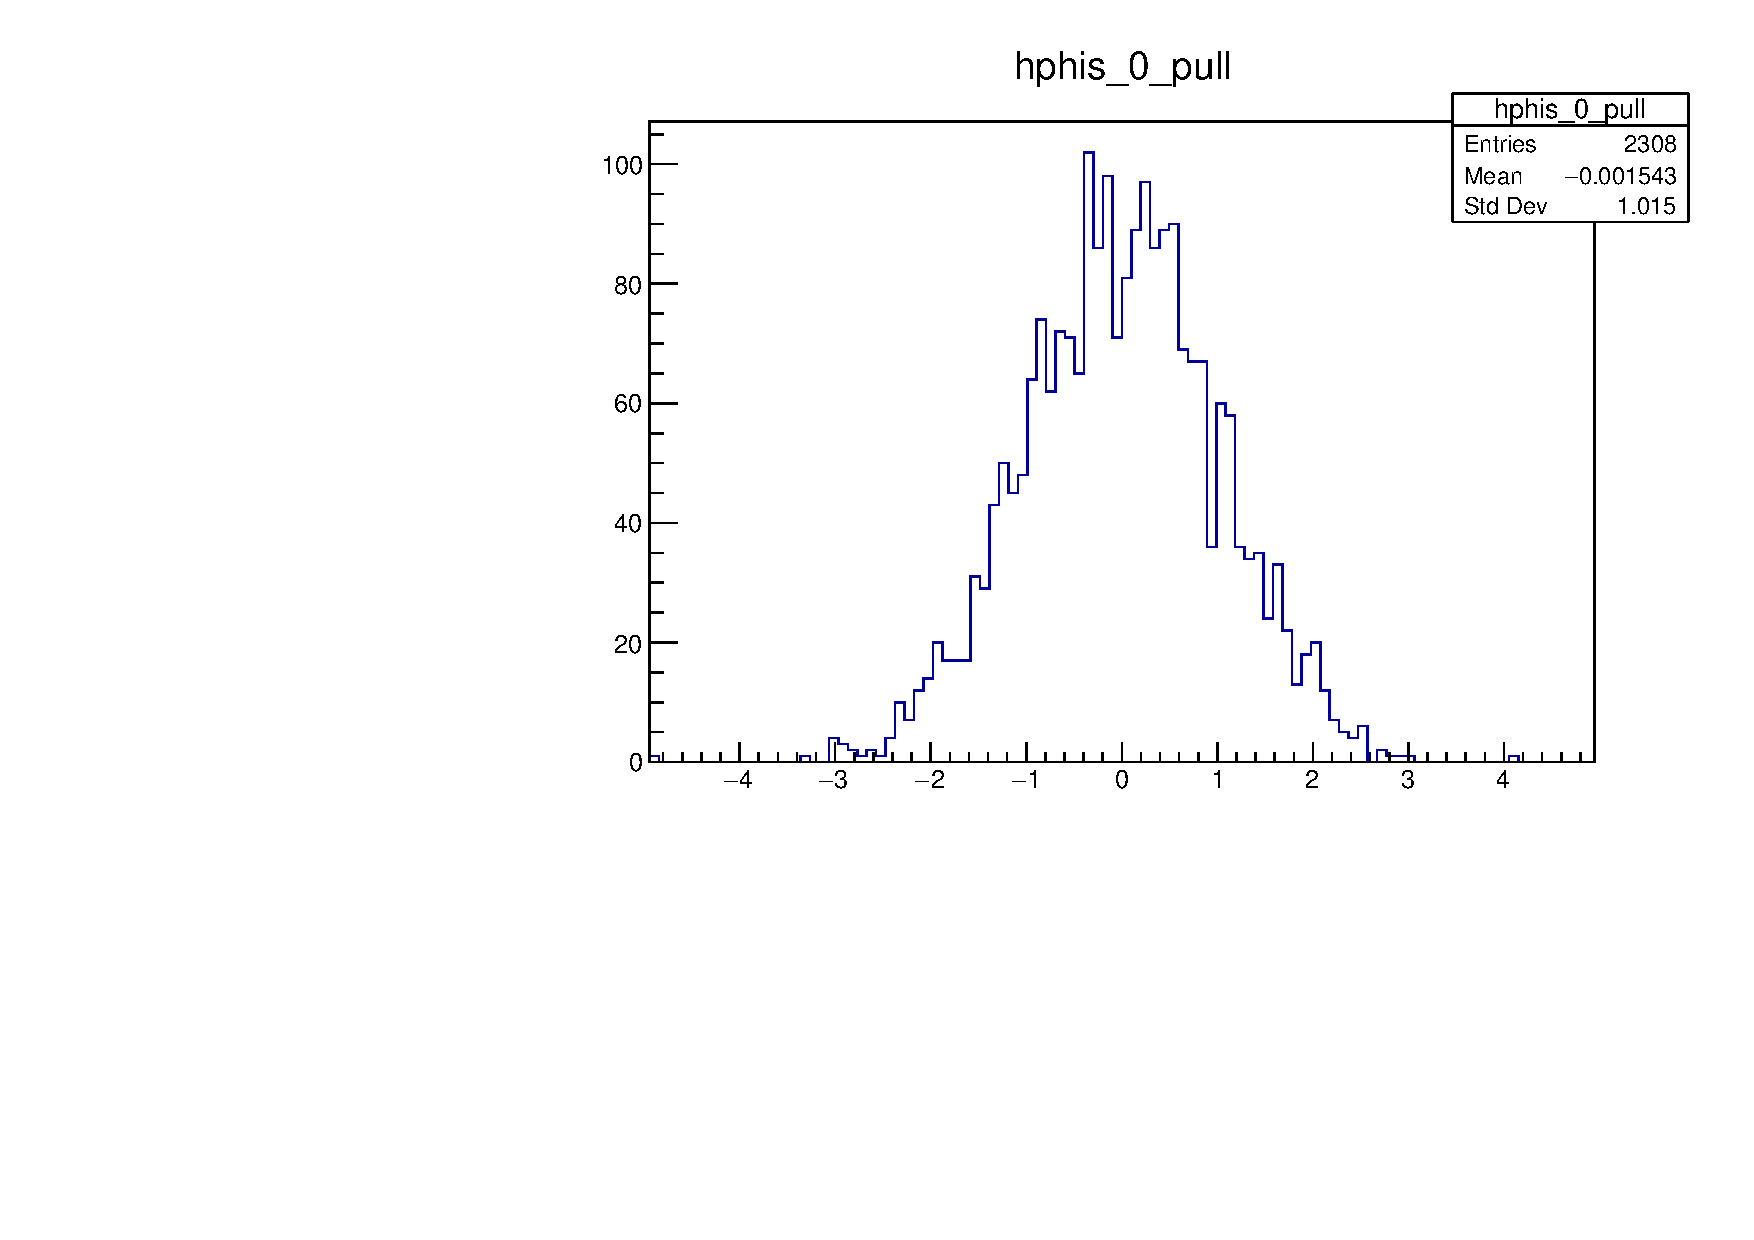
\includegraphics[width=0.3\textwidth]{figs/DataPulls/phis_0_pull.pdf}
	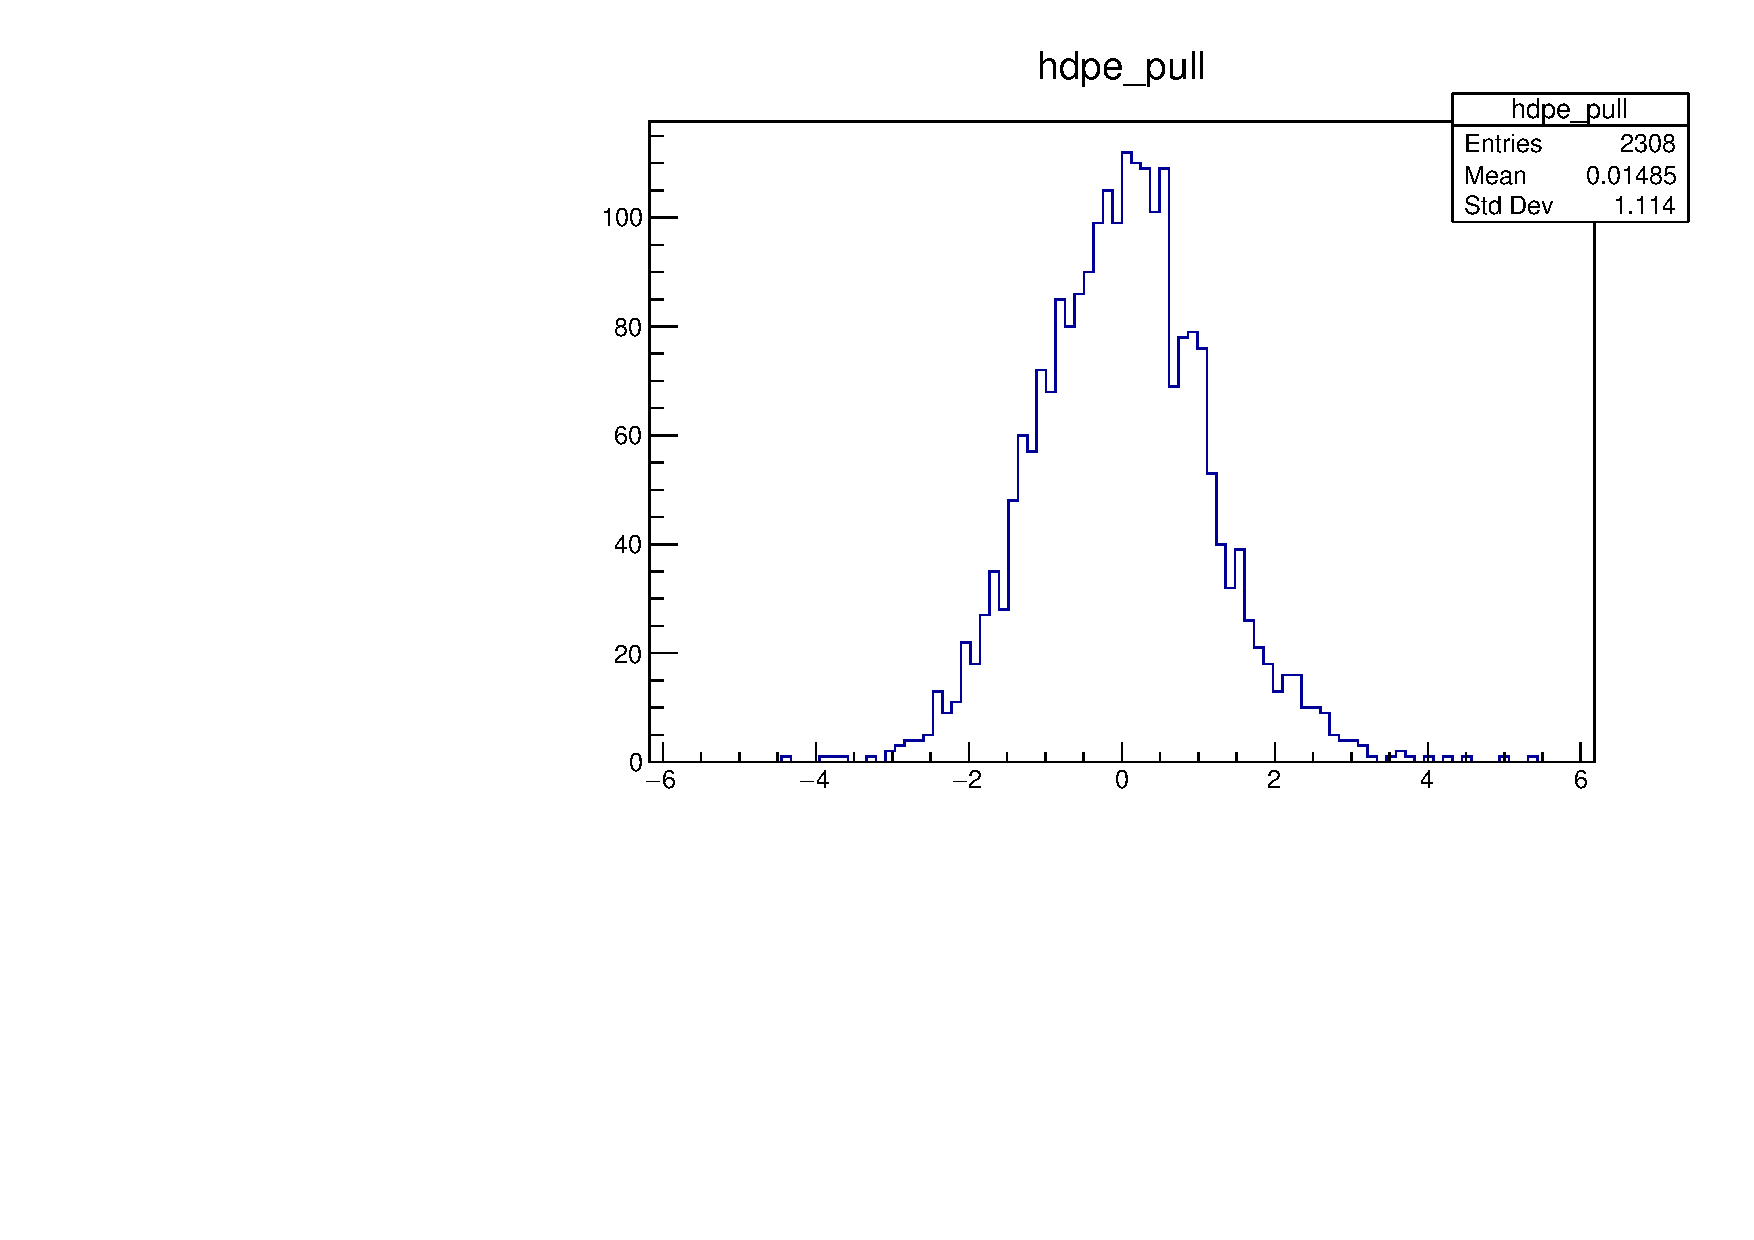
\includegraphics[width=0.3\textwidth]{figs/DataPulls/dpe_pull.pdf}
	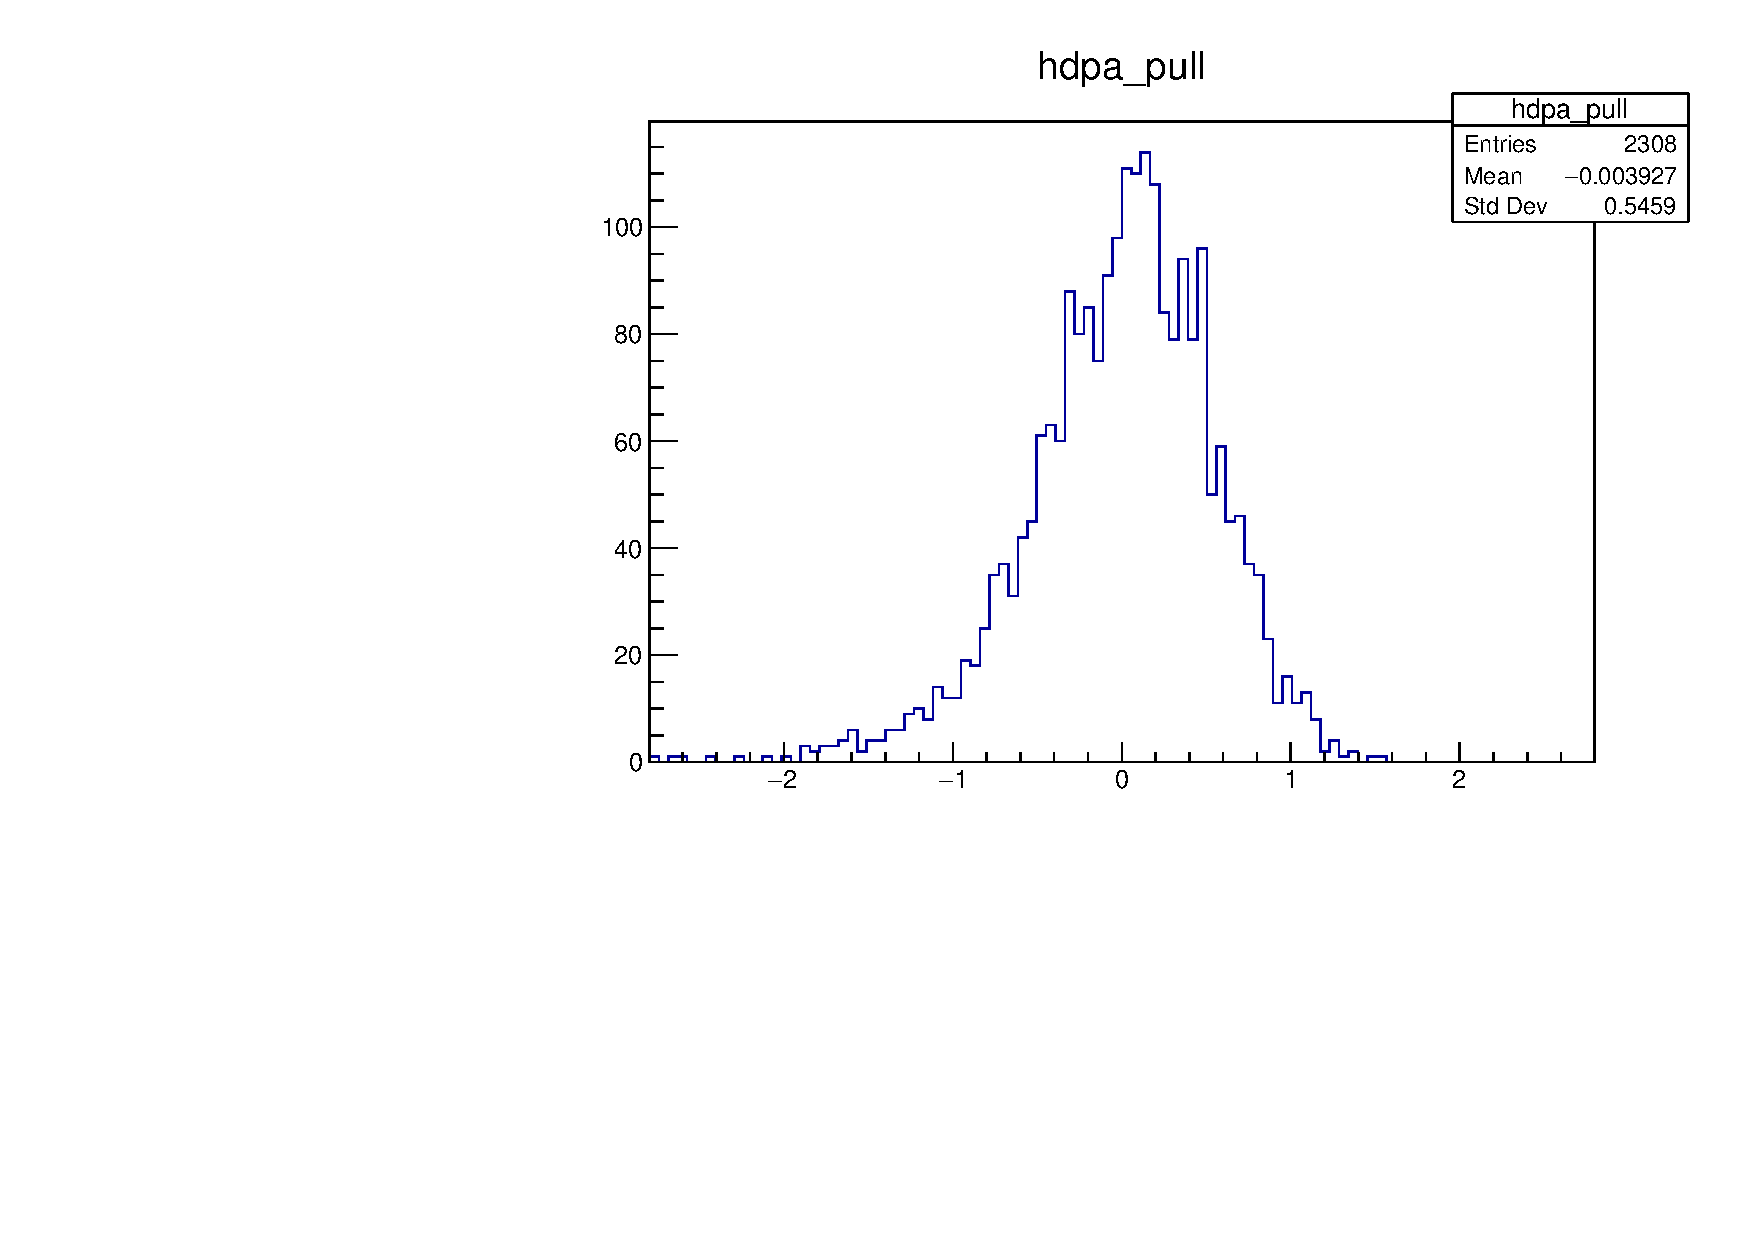
\includegraphics[width=0.3\textwidth]{figs/DataPulls/dpa_pull.pdf}
	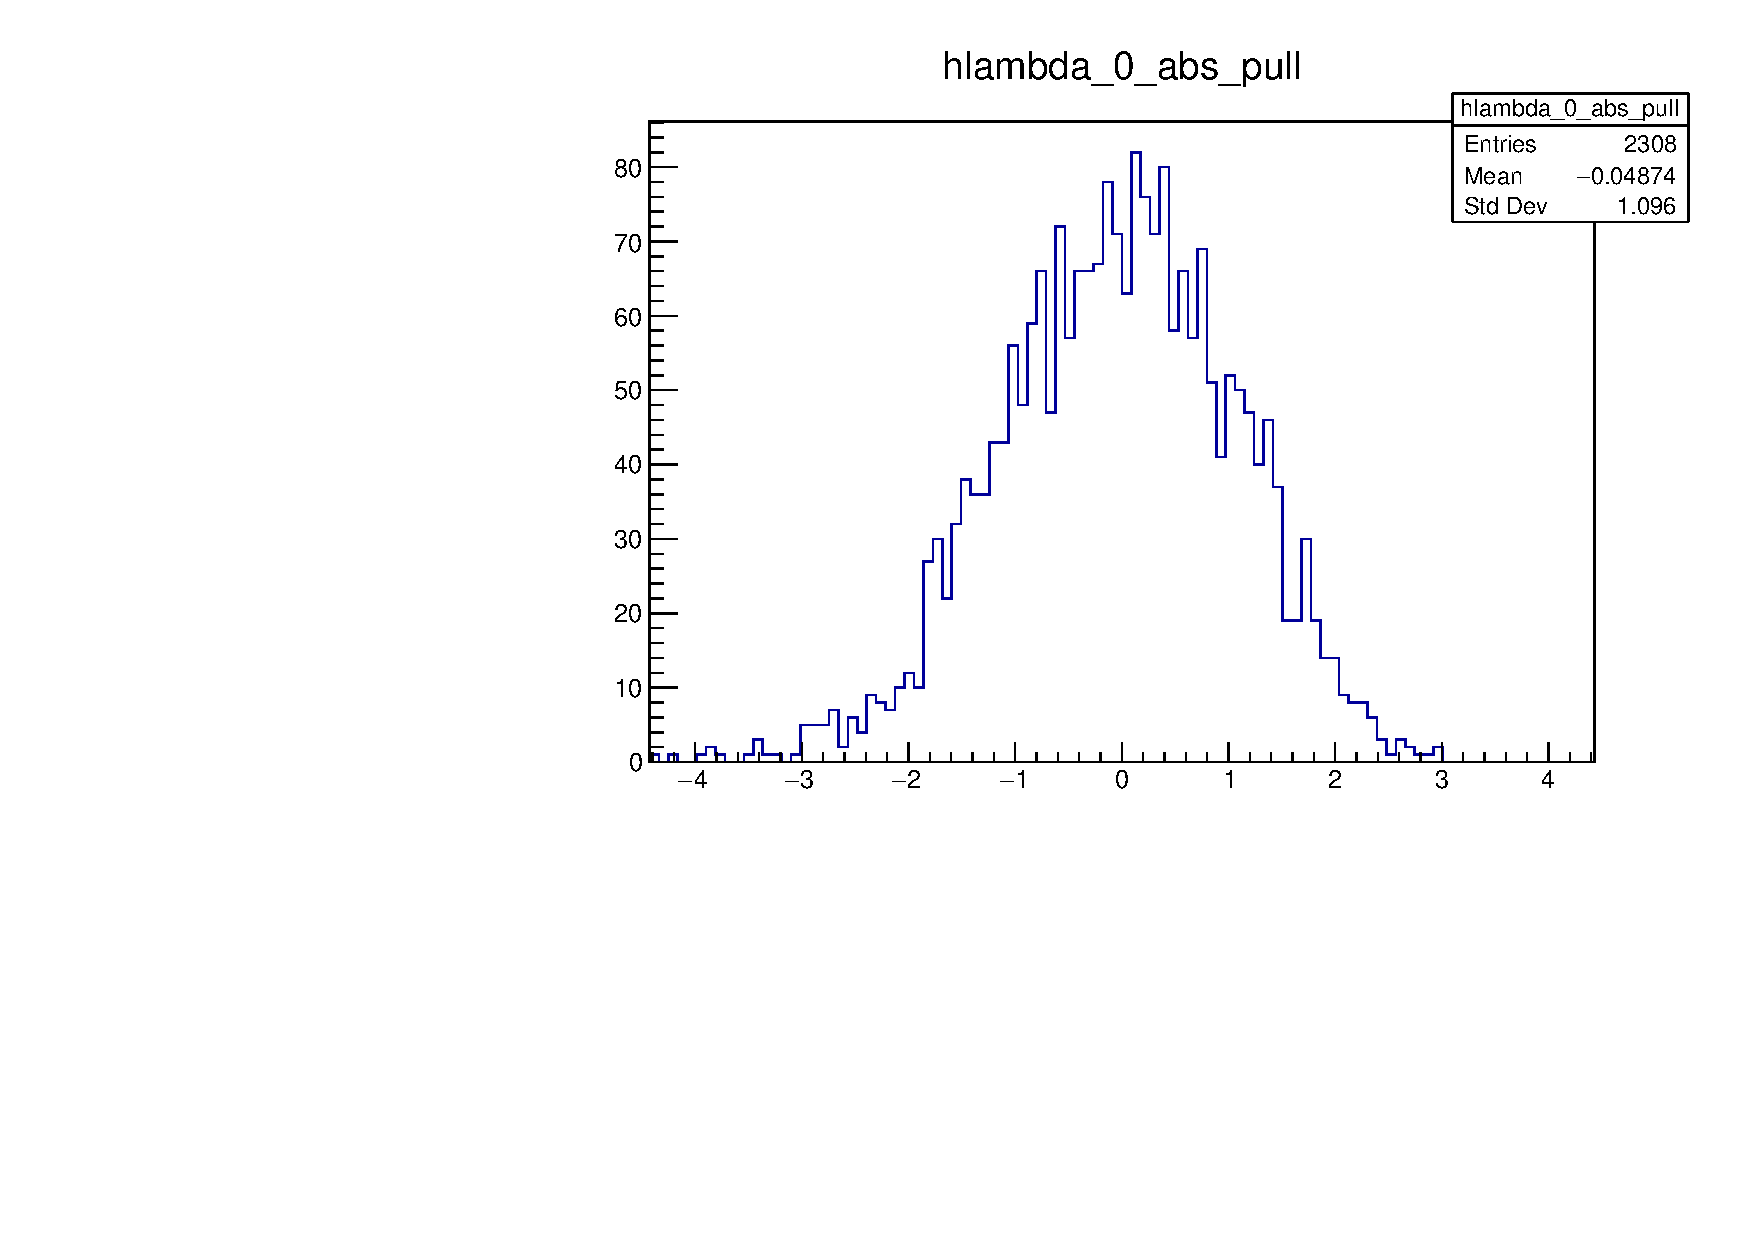
\includegraphics[width=0.3\textwidth]{figs/DataPulls/lambda_0_abs_pull.pdf}
	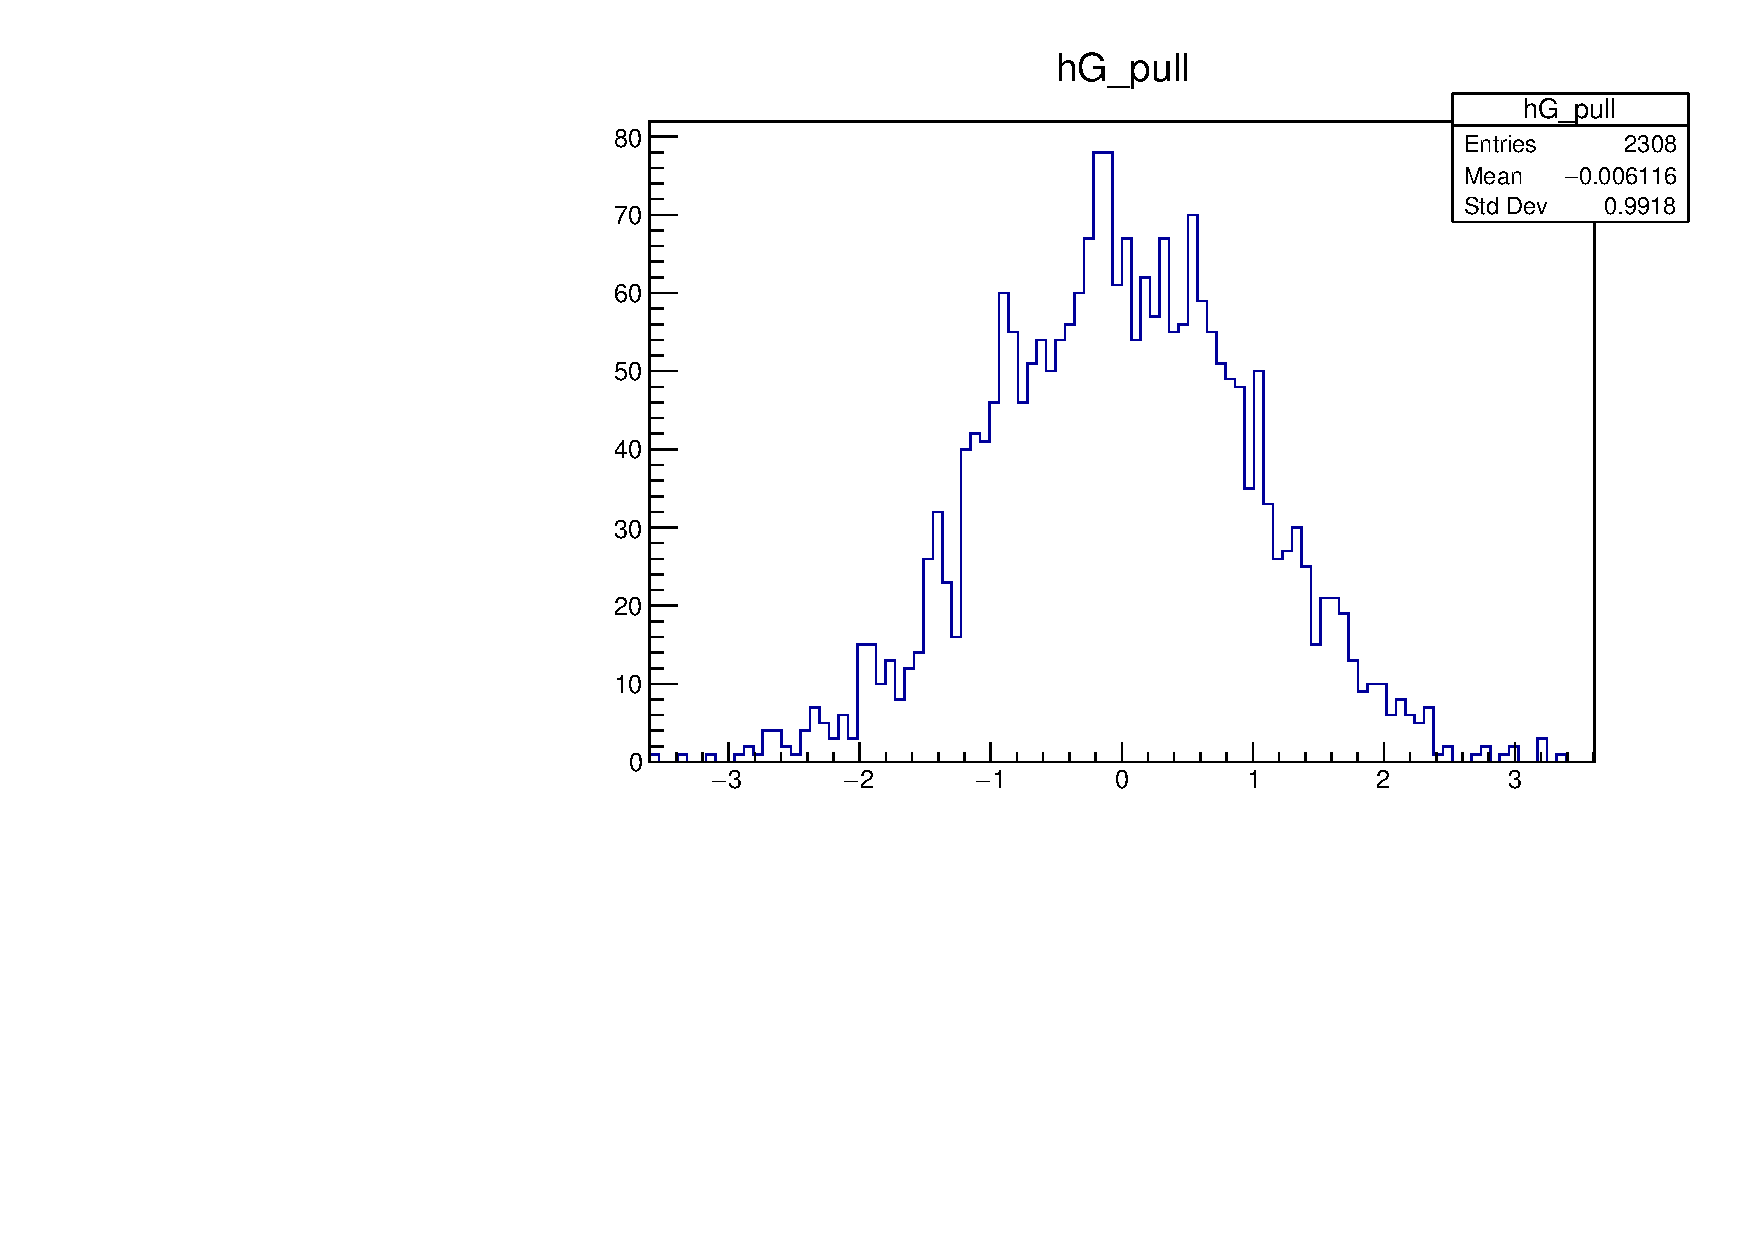
\includegraphics[width=0.3\textwidth]{figs/DataPulls/G_pull.pdf}
	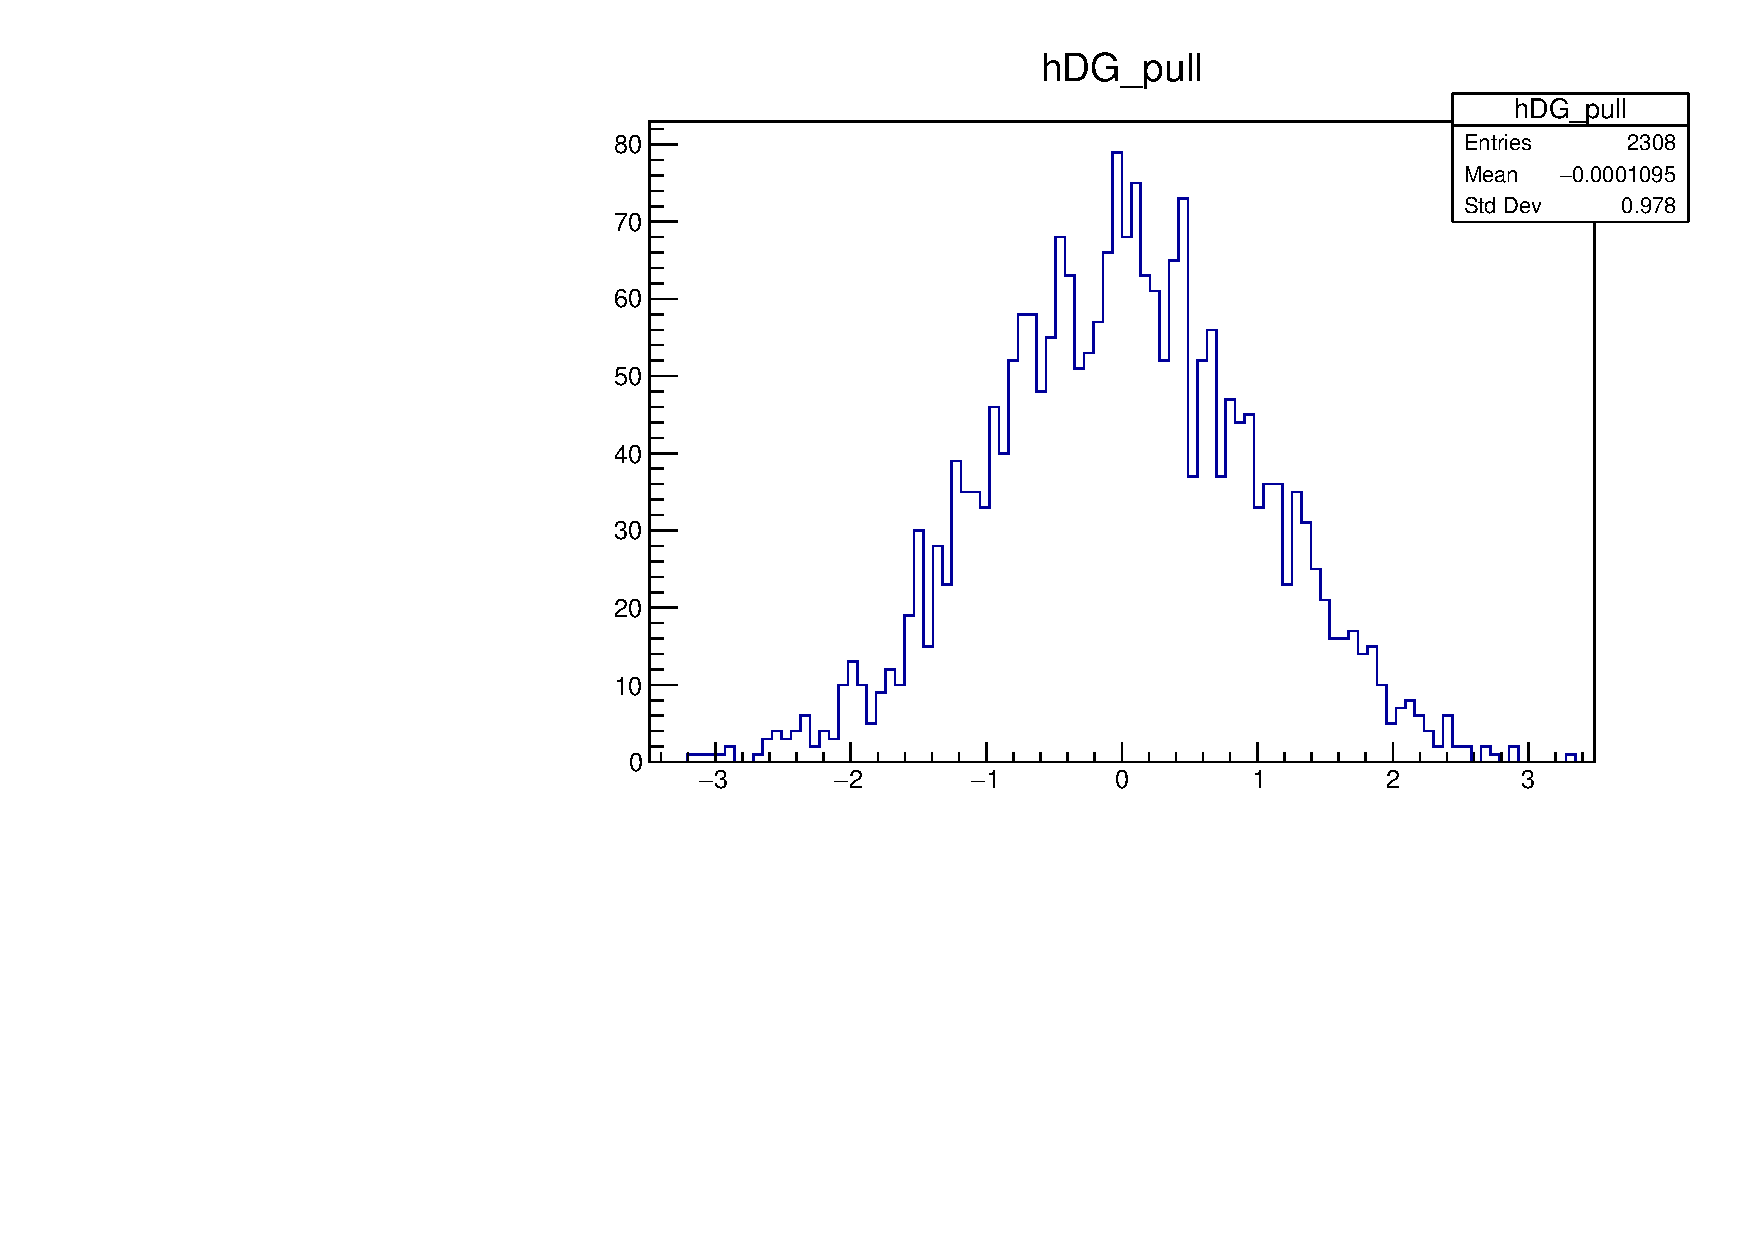
\includegraphics[width=0.3\textwidth]{figs/DataPulls/DG_pull.pdf}
	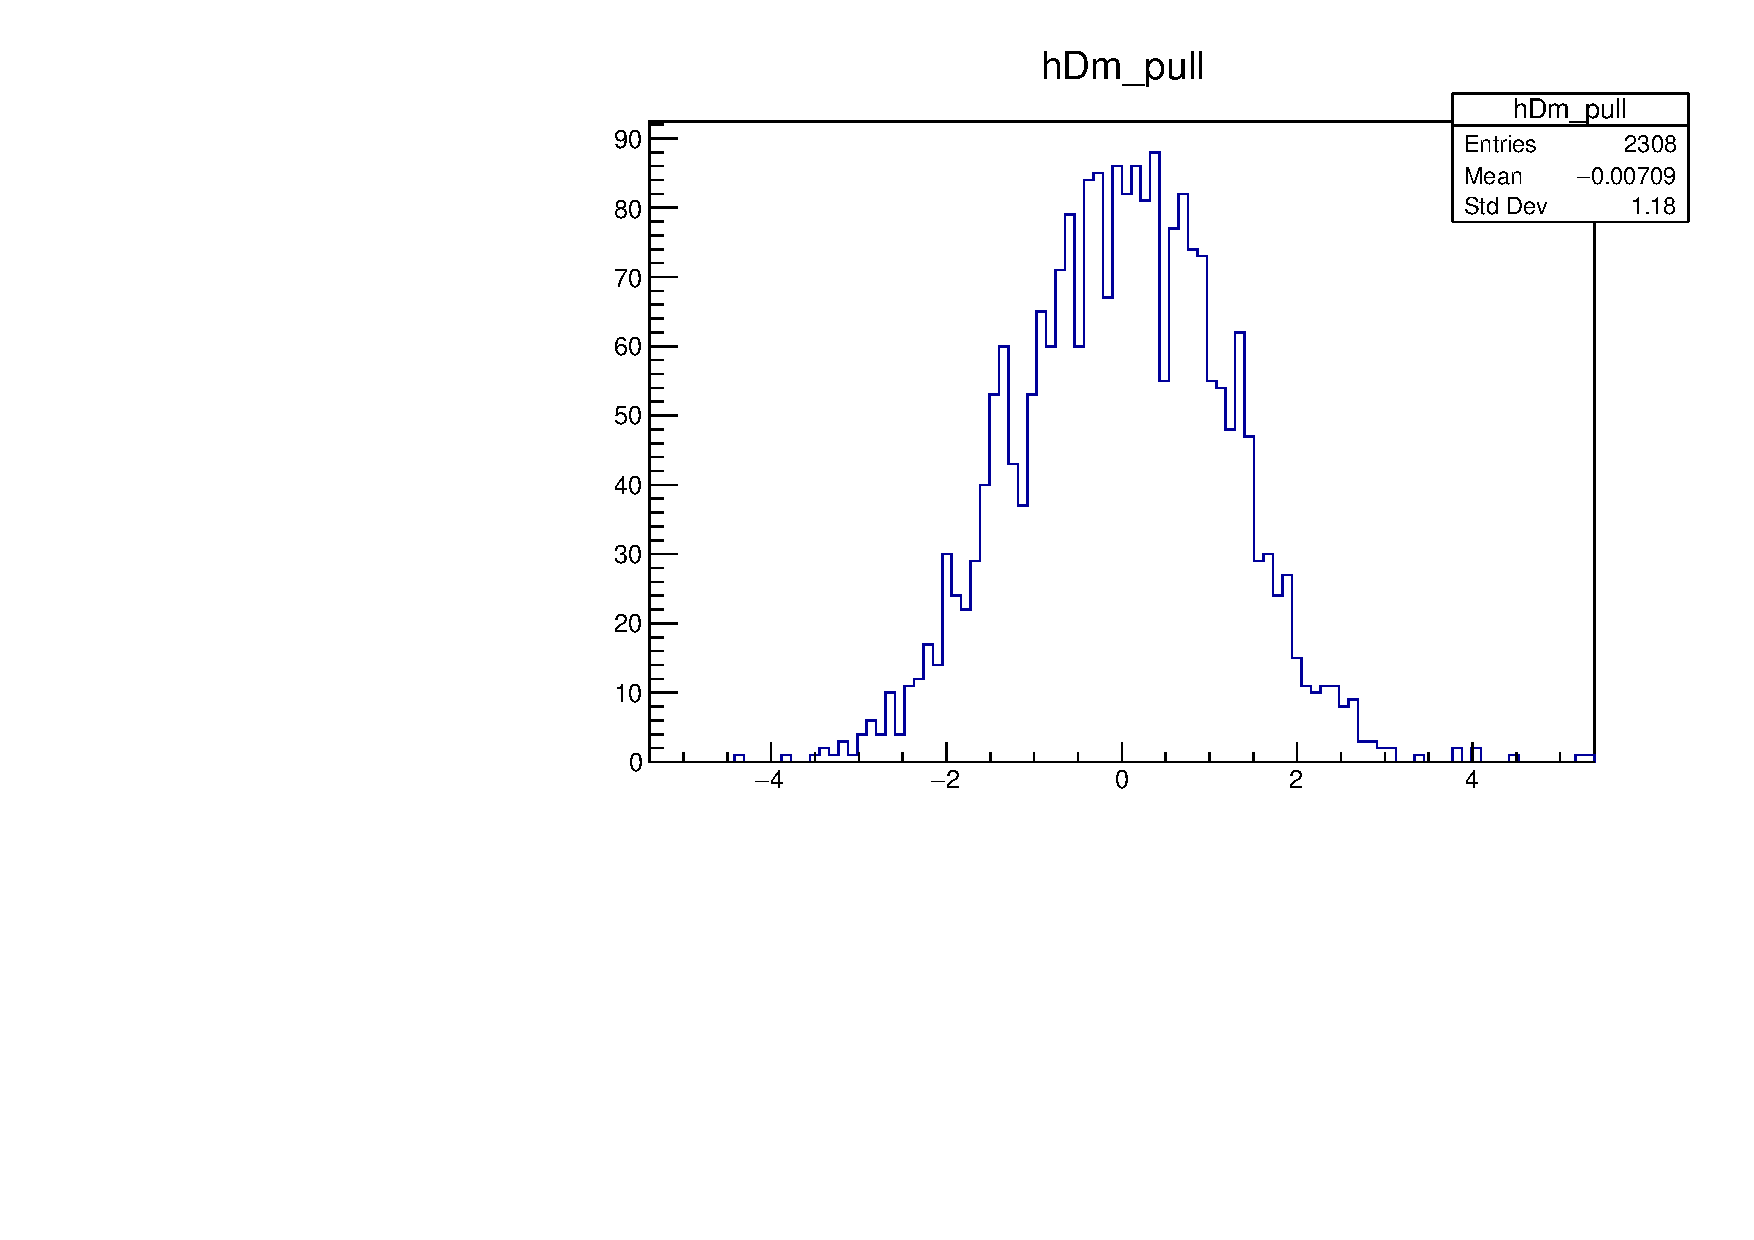
\includegraphics[width=0.3\textwidth]{figs/DataPulls/Dm_pull.pdf}
	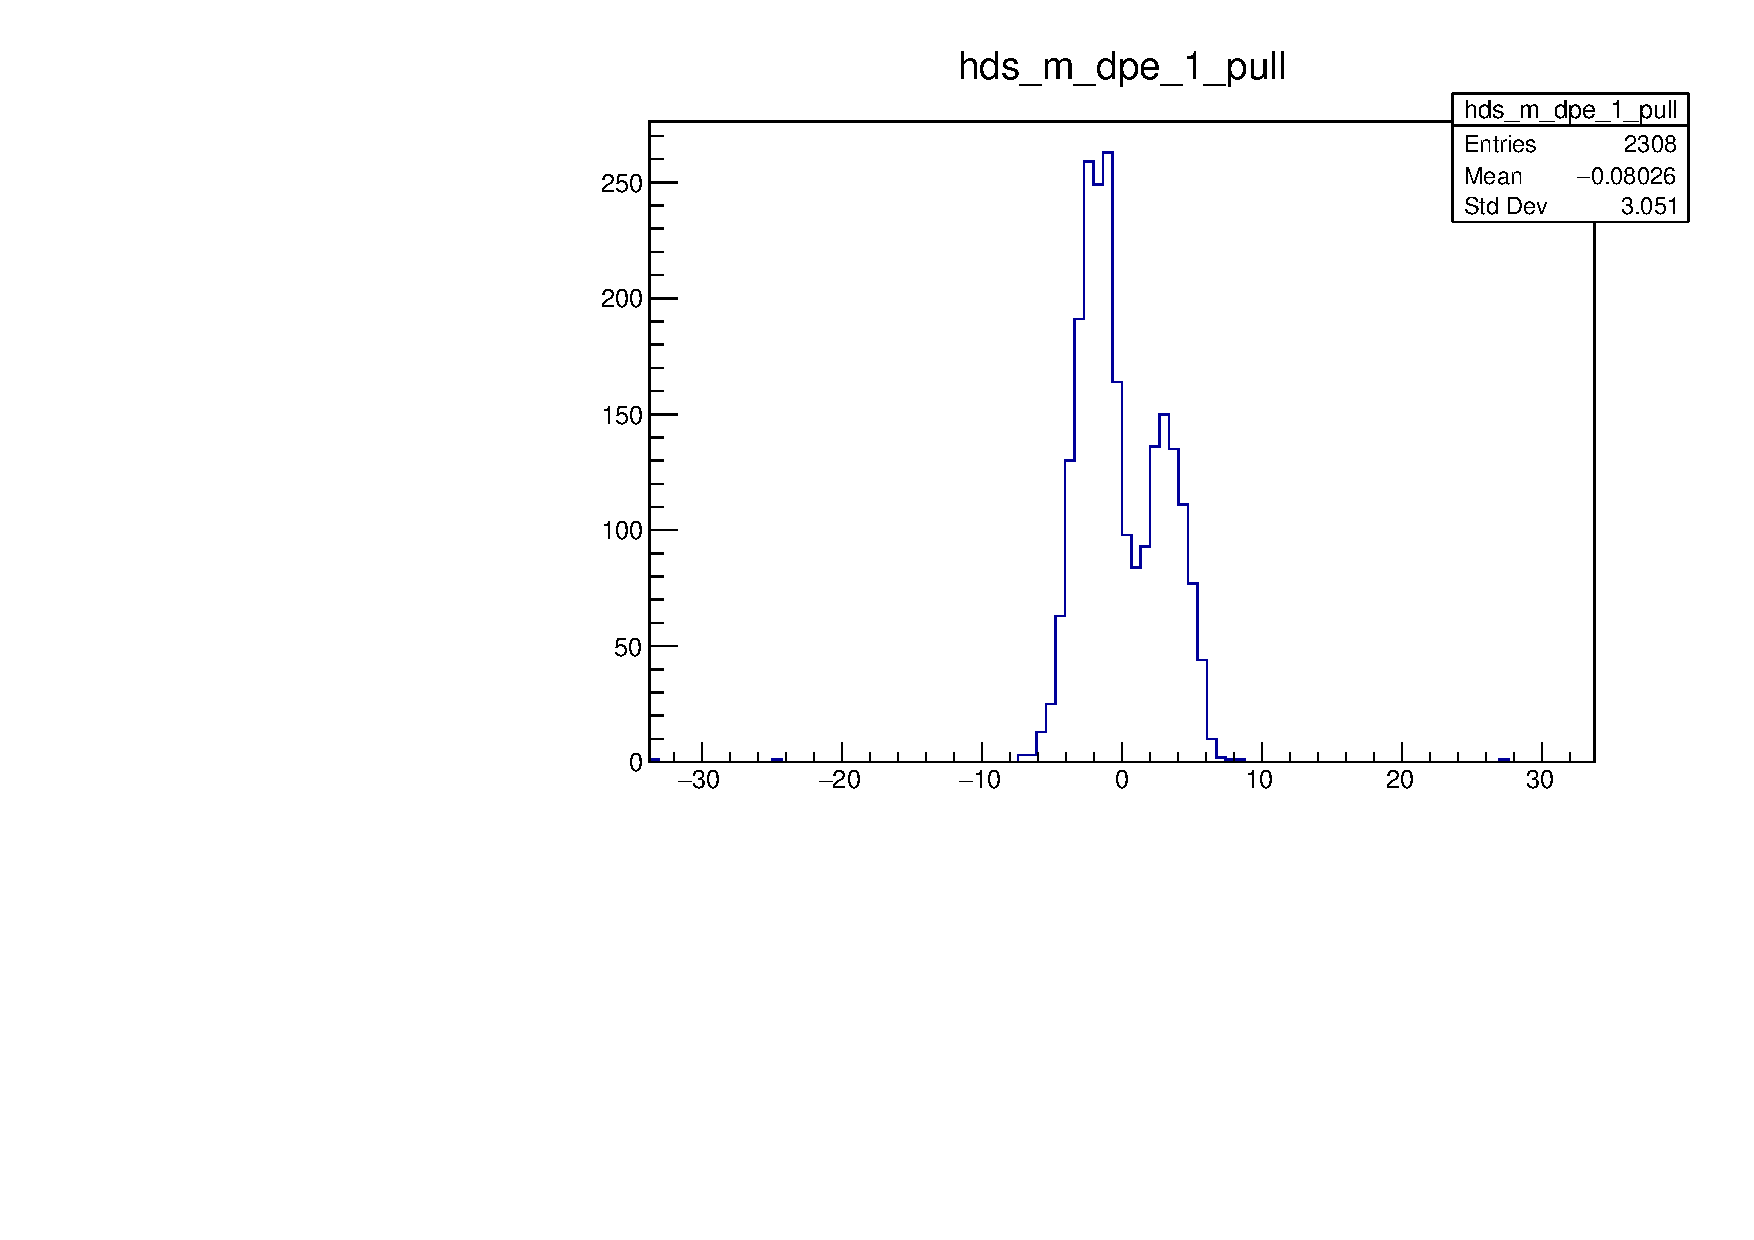
\includegraphics[width=0.3\textwidth]{figs/DataPulls/ds_m_dpe_1_pull.pdf}
	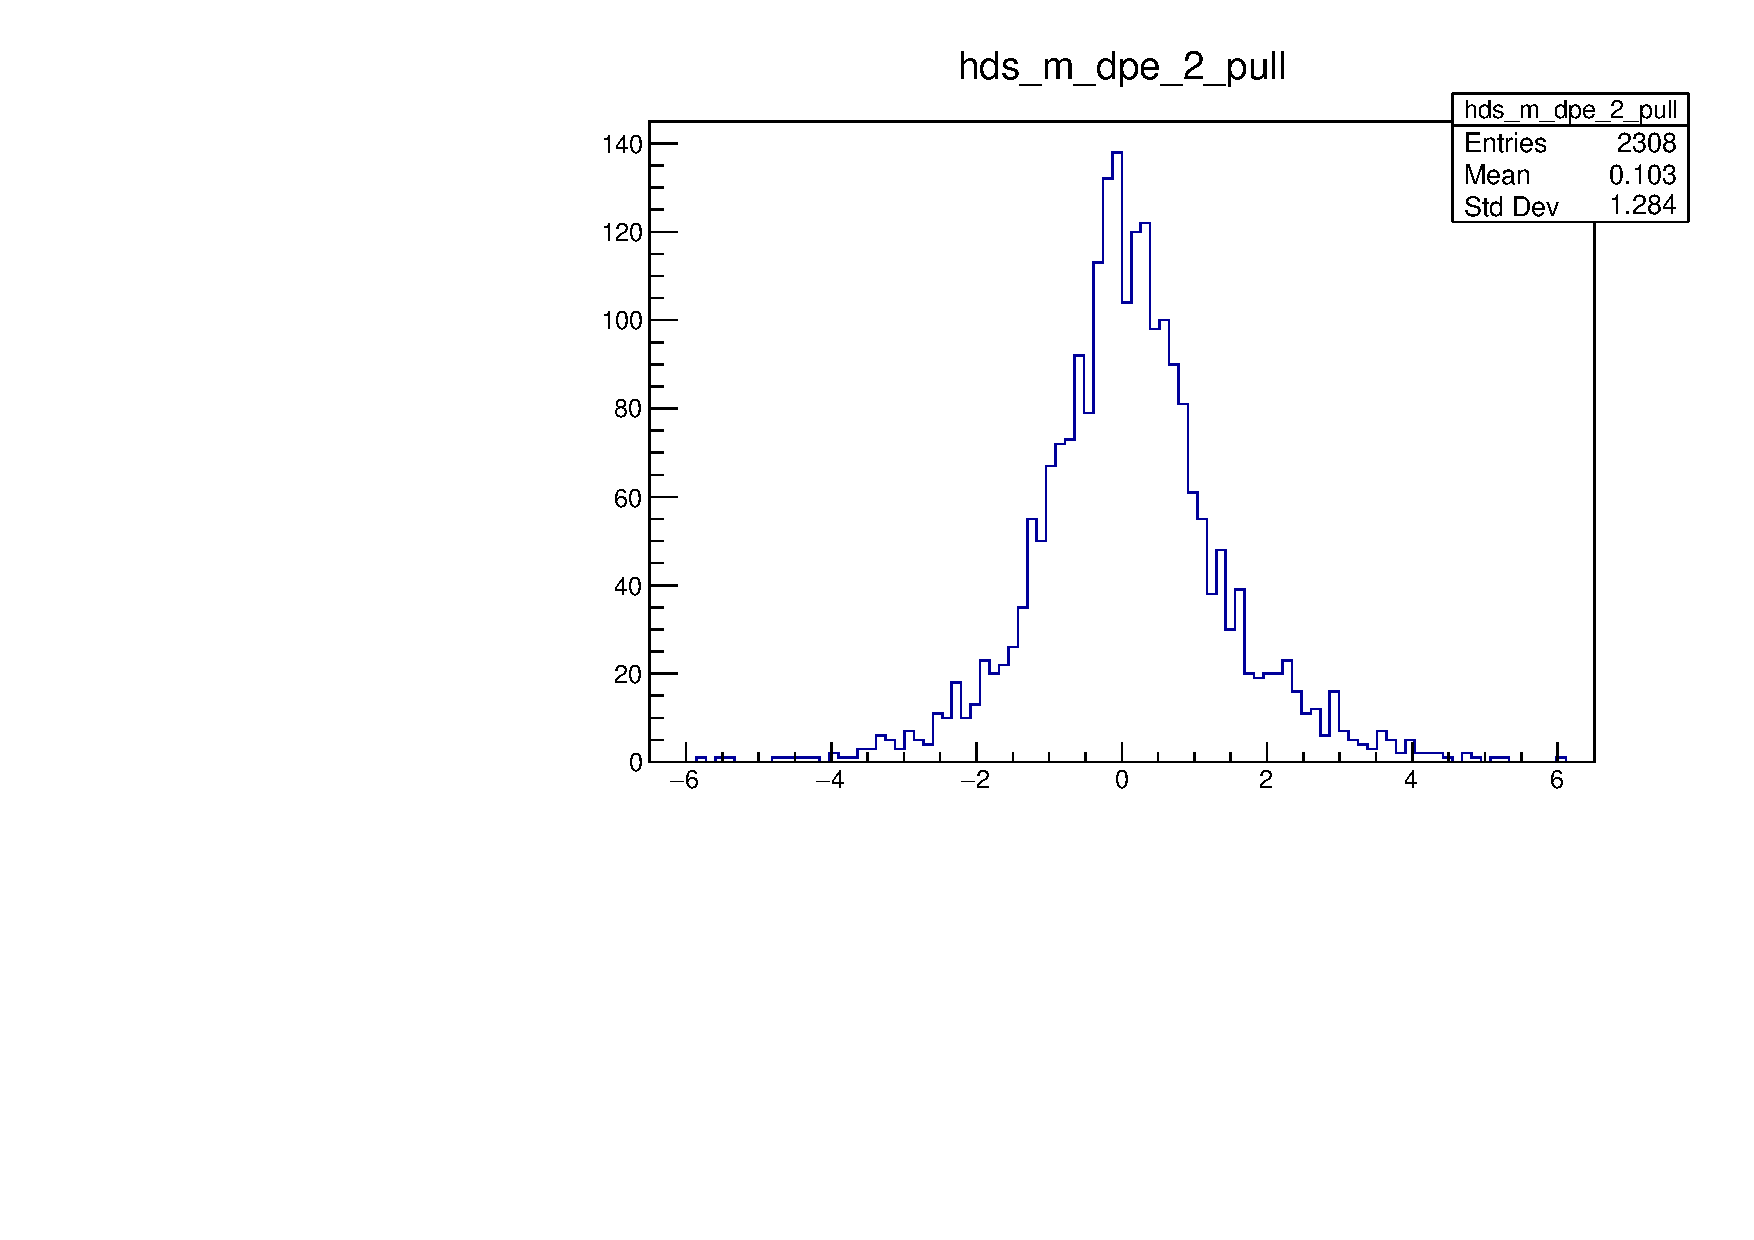
\includegraphics[width=0.3\textwidth]{figs/DataPulls/ds_m_dpe_2_pull.pdf}
	\includegraphics[width=0.3\textwidth]{figs/DataPulls/ds_m_dpe_3_pull.pdf}
	\includegraphics[width=0.3\textwidth]{figs/DataPulls/ds_m_dpe_4_pull.pdf}
	\includegraphics[width=0.3\textwidth]{figs/DataPulls/ds_m_dpe_5_pull.pdf}
	\includegraphics[width=0.3\textwidth]{figs/DataPulls/ds_m_dpe_6_pull.pdf}
	\includegraphics[width=0.3\textwidth]{figs/DataPulls/Fs_1_pull.pdf}
	\includegraphics[width=0.3\textwidth]{figs/DataPulls/Fs_2_pull.pdf}
	\includegraphics[width=0.3\textwidth]{figs/DataPulls/Fs_3_pull.pdf}
	\includegraphics[width=0.3\textwidth]{figs/DataPulls/Fs_4_pull.pdf}
	\includegraphics[width=0.3\textwidth]{figs/DataPulls/Fs_5_pull.pdf}
	\includegraphics[width=0.3\textwidth]{figs/DataPulls/Fs_6_pull.pdf}
   \end{center}
   \caption{
	Pull distributions of the fit parameters using bootstrapping (data).
       Pulls are computed relative to data central values.
   }
   \label{fig:Pulls_Data}
\end{figure}

\begin{figure}[tb]
   \begin{center}
	\includegraphics[width=0.3\textwidth]{figs/MCwBkgVars/fL_var.pdf}
	\includegraphics[width=0.3\textwidth]{figs/MCwBkgVars/fpe_var.pdf}
	\includegraphics[width=0.3\textwidth]{figs/MCwBkgVars/phis_0_var.pdf}
	\includegraphics[width=0.3\textwidth]{figs/MCwBkgVars/dpe_var.pdf}
	\includegraphics[width=0.3\textwidth]{figs/MCwBkgVars/dpa_var.pdf}
	\includegraphics[width=0.3\textwidth]{figs/MCwBkgVars/lambda_0_abs_var.pdf}
	\includegraphics[width=0.3\textwidth]{figs/MCwBkgVars/Gs_m_Gd_var.pdf}
	\includegraphics[width=0.3\textwidth]{figs/MCwBkgVars/DG_var.pdf}
	\includegraphics[width=0.3\textwidth]{figs/MCwBkgVars/Dm_var.pdf}
   \end{center}
   \caption{
	Distributions of the fit parameters using bootstrapping (simulation and background simulation).
   }
   \label{fig:Vars_MCwBkg}
\end{figure}

\begin{figure}[tb]
   \begin{center}
	\includegraphics[width=0.3\textwidth]{figs/MCwBkgPulls/fL_pull.pdf}
	\includegraphics[width=0.3\textwidth]{figs/MCwBkgPulls/fpe_pull.pdf}
	\includegraphics[width=0.3\textwidth]{figs/MCwBkgPulls/phis_0_pull.pdf}
	\includegraphics[width=0.3\textwidth]{figs/MCwBkgPulls/dpe_pull.pdf}
	\includegraphics[width=0.3\textwidth]{figs/MCwBkgPulls/dpa_pull.pdf}
	\includegraphics[width=0.3\textwidth]{figs/MCwBkgPulls/lambda_0_abs_pull.pdf}
	\includegraphics[width=0.3\textwidth]{figs/MCwBkgPulls/Gs_m_Gd_pull.pdf}
	\includegraphics[width=0.3\textwidth]{figs/MCwBkgPulls/DG_pull.pdf}
	\includegraphics[width=0.3\textwidth]{figs/MCwBkgPulls/Dm_pull.pdf}
   \end{center}
   \caption{
	Pull distributions of the fit parameters using bootstrapping (signal and background simulation).
   }
   \label{fig:Pulls_MCwBkg}
\end{figure}
\clearpage
